%%%%%%%%%%%%%%%%%%%%%%%%%%%%%%%%%%%%%%%%%%%%%%%%%%%%%%%%%%%%%%%%%%%%%%%%%%%%%%%%
%2345678901234567890123456789012345678901234567890123456789012345678901234567890
%        1         2         3         4         5         6         7         8

\documentclass[letterpaper, 10 pt, conference]{ieeeconf}  % Comment this line out if you need a4paper

%\documentclass[a4paper, 10pt, conference]{ieeeconf}      % Use this line for a4 paper

\IEEEoverridecommandlockouts                              % This command is only needed if 
                                                          % you want to use the \thanks command

\overrideIEEEmargins                                      % Needed to meet printer requirements.

% See the \addtolength command later in the file to balance the column lengths
% on the last page of the document

% The following packages can be found on http:\\www.ctan.org
%\usepackage{graphics} % for pdf, bitmapped graphics files
%\usepackage{epsfig} % for postscript graphics files
%\usepackage{mathptmx} % assumes new font selection scheme installed
%\usepackage{times} % assumes new font selection scheme installed
%\usepackage{amsmath} % assumes amsmath package installed
%\usepackage{amssymb}  % assumes amsmath package installed
\usepackage[noadjust]{cite}
\usepackage{graphicx}                
\usepackage{array,graphicx,float,caption}
\usepackage{subcaption}
\usepackage{booktabs}
\usepackage[normalem]{ulem}
% packages needed for Perla's commands
\usepackage{color}
\usepackage{soul}
\usepackage{array, amsmath}
\usepackage{bm}

\useunder{\uline}{\ul}{}

%Commands defined by Perla
\newcommand{\DelP}[1]{\textcolor{red}{\st{#1}}}
\newcommand{\AddP}[1]{\textcolor{blue}{#1}}
\newcommand{\NoteP}[1]{\textcolor{green}{#1}}
\newcommand{\ULsubfloat}[2][\empty]% #1 = caption (optional), #2 = image
{\hbox{% unbreakable group
		\sbox0{#2}% measure height of image
		\captionsetup{position=top, justification=raggedleft, singlelinecheck=false}%
		\rotatebox[origin=bl]{90}{\begin{minipage}[b]{\dimexpr \ht0+\dp0}
				\subcaption{#1}
		\end{minipage}}\raisebox{\dp0}{\usebox0}%
}}

\title{\LARGE \bf
	Soft Morphological Processing of Tactile Stimuli \\for Autonomous Category Formation
}


\author{Luca Scimeca$^{1}$, Perla Maiolino$^{1}$ and Fumiya Iida$^{1}$% <-this % stops a space
\thanks{*This work was funded by the UK Agriculture and Horticulture Development Board and by The United Kingdom Engineering and Physical Sciences Research Council (EPSRC) MOTION grant [EP/N03211X/2].}% <-this % stops a space
\thanks{$^{1}$ L. Scimeca, P. Maiolino and F. Iida are with the Machine Intelligence Laboratory, �
	Department of Engineering, University of Cambridge, Trumpington Street,
	CB2 1PZ, Cambridge UK, Email {\tt\small ls769@cam.ac.uk}, {\tt\small pm640@cam.ac.uk},	
	{\tt\small fi224@cam.ac.uk.}
        }%%
}


\begin{document}



\maketitle
\thispagestyle{empty}
\pagestyle{empty}


%%%%%%%%%%%%%%%%%%%%%%%%%%%%%%%%%%%%%%%%%%%%%%%%%%%%%%%%%%%%%%%%%%%%%%%%%%%%%%%%
\begin{abstract}
		Sensor morphology is a fundamental aspect of tactile sensing technology. Design choices induce stimuli to be morphologically processed, changing the sensory perception of the touched objects and affecting inference at a later processing stage. We develop a framework to analyze the filtered sensor response and observe the correspondent change in tactile information. We test the morphological processing effects on the tactile stimuli by integrating a capacitive tactile sensor into a flat end-effector and creating three soft silicon-based filters with varying thickness ($\bm{3mm}$, $\bm{6mm}$ and $\bm{10mm}$). We incorporate the end-effector onto a robotic arm. We control the arm in order to apply a calibrated force onto 4 objects, and retrieve tactile images. We create an unsupervised inference process through the use of Principal Component Analysis and K-Means Clustering. We use the process to group the sensed objects into 2 classes and observe how different soft filters affect the clustering results. The sensor response with the $\bm{3mm}$ soft filter allows for edges to be the feature with most variance (captured by $\bm{PCA}$) and induces the association of edged objects. With thicker soft filters the associations change, and with a $\bm{10mm}$ filter the sensor response results more diverse for objects with different elongation. We show that the clustering is intrinsically driven by the morphology of the sensor and that the robot's world understanding changes according to it.
\end{abstract}


%%%%%%%%%%%%%%%%%%%%%%%%%%%%%%%%%%%%%%%%%%%%%%%%%%%%%%%%%%%%%%%%%%%%%%%%%%%%%%%%
\section{INTRODUCTION}

The somatosensory system of biological organisms decodes, interprets and categorizes a wide range of tactile stimuli arising from interactions with the environment.
%The somatosensory system of biological organisms decodes and interprets a wide range of tactile stimuli arising from interactions with the environment, providing the ability to categorise them and to react accordingly.
This difficult task, if in part achieved at a neural level, is known to be initially performed at sensory receptor's level \cite{Ahissar_2016}.
%The ability to decode and categorise stimulation (e.g., to detect the invariants in it) is not trivial. Part of this ability is learned coming repeatedly in contact with the stimulus and it is performed at neural level (e.g., we are able to distinguish a caress from a warm breeze), but it has been demonstrated that part of this decoding is performed at sensory organs level. 
As an example, the morphology of the vibrissal system of rats is useful in extracting information relative to object texture, orientation, shape, size and location of surfaces. The system then, preprocesses information from the environment into useful stimuli to be further processed by the brain \cite{Bagdasarian_2013}.
%For example in rats, vibrissal system extracts information needed to accurately interpret interactions with the environment and to determine objects texture, compliance, orientation, shape, size and location (paper to cite "Pre-neuronal morphological processing of object location by individual whiskers"). 
In humans, when a scene is explored by touch, the morphology of the skin (in particular of the $Meissner's\ Corpuscles$ together with the $Dermal\ Papillae$) allows the encoding of edge information \cite{Chorley_2009}.
%In humans, the morphology of skin (in purticular morphology of Meissner's Corpuscles together with Dermal Papillae) allows the encoding of edge information during touch exploration of a scene (paper to cite "Development of a Tactile Sensor Based on Biologically Inspired Edge Encoding").\\
\noindent In the last decades, substantial efforts have been made in enhancing the perceptions capabilities of robots by providing them with a sense of touch \cite{dahiya_tactile_2010}. 
Despite the large number of tactile sensors developed, the proposed solutions have been often presented at a prototypical level, where the designs needed be specifically tailored to individual robots and applications. In this context, design principles would be focused on finding trade-offs between aspects such as transduction principles, sensor performances and ease of integration, but only a limited number of research work, mainly in the soft robotics community, have focused on the development of tactile sensors with functional morphology \cite{Hughes_2017, Lepora_2017, culha2014svas3}. A structured research review about the use of sensor morphology in robotic systems can be found in \cite{fumiya_2016}.
Despite the efforts, the role of sensor morphology in encoding and categorizing touch stimuli remains a significant challenge. The interpretation of the sensor signals to discriminate between a set of stimuli or to perform object recognition has relied mainly on supervised machine learning techniques \cite{Gastaldo_2015, Silvera_2012, Kaboli_2015}, burdening solutions with the need of large amount of labeled data. 
%As already demonstrated in biological organisms, sensor morphology plays a  central role in perception \cite{pfeifer_2014, pfeifer_how_2006, fend_2006}, directly affecting the way stimuli from the environment are transduced in signals to be further processed by the brain. Analogously, the sensor morphology in a robot can affect the sensed characteristics of objects, and consequently the way in which robots $see$ the world \cite{lichtensteiger_need_2004, Nakajima_2015}. 
The main contribution of this paper is to propose a conceptual framework to examine whether any processing or meaningful transformation occurs in robotic tactile sensing due to its morphology and, consequently, how morphological processing can drive the robot's internal representation of the world. This work marks a step towards the design of sensors whose morphology can sensibly aid in the information processing of perceptual inputs for a task at hand.
%In particular, we set a framework where objects, with different geometrical characteristics, are sensed through an end effector, coupled with a tactile sensor with different soft filters. The change in morphology induced by the covers processes the sensory response before a central processing system can make inference. In order not to bias the information change induced by the processed sensory response, we exercise the inference process in an unsupervised manner i.e. clustering (Fig \ref{conceptual_map}).
\begin{figure}[]
	\centering
	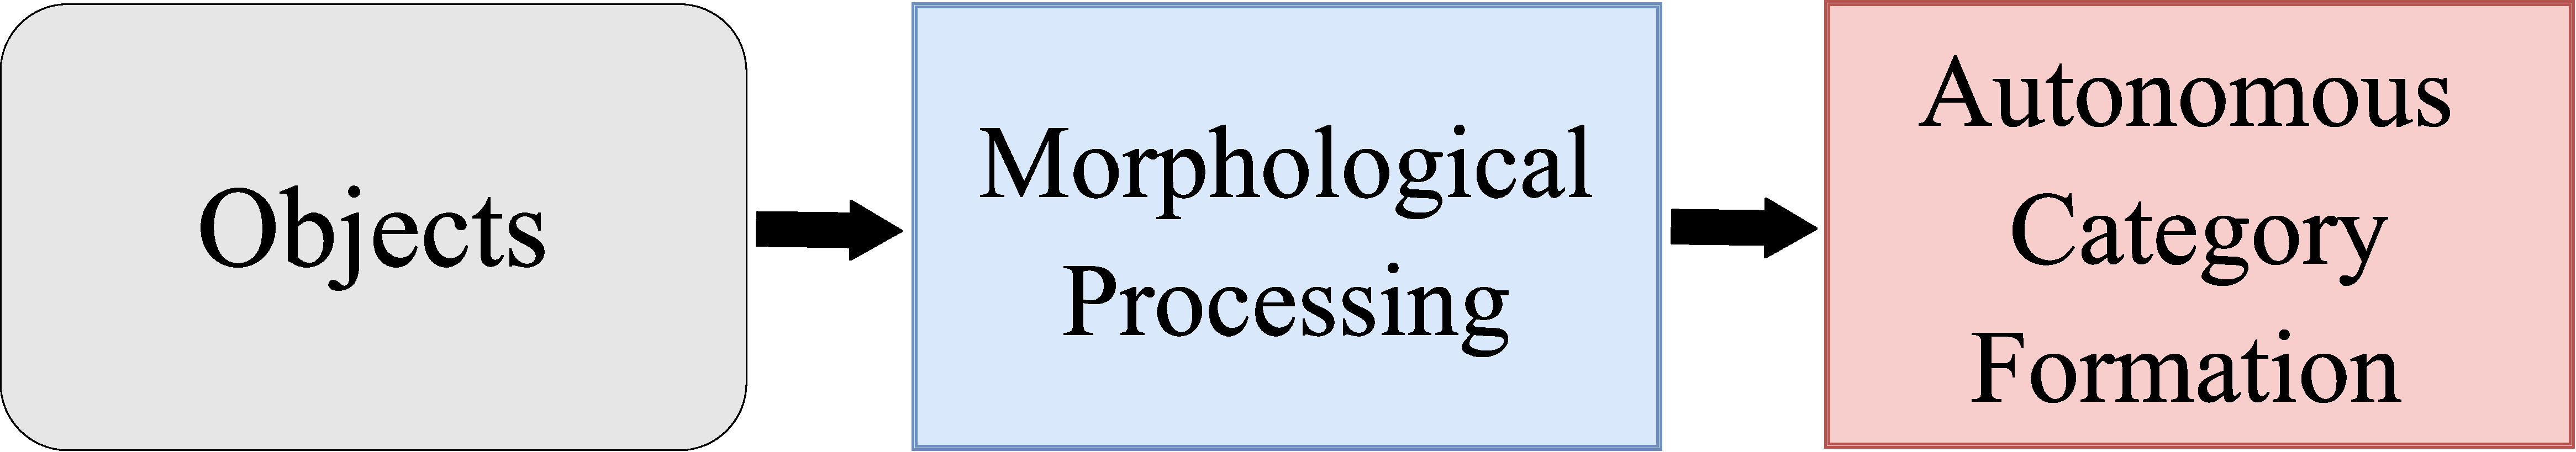
\includegraphics[width=.48\textwidth]{./figs/conceptual_map}
	\caption{Conceptual map for the Morphological Processing of Sensory Receptors.}
	\label{conceptual_map}
\end{figure}

To actualize the conceptual framework, we consider a learning problem of tactile discrimination tasks, in which a robot should acquire categories of tactile sensing information induced by different types of objects physically in contact. We consider these categories to be autonomously generated through unsupervised clustering of sensory information. The way in which the robot clusters the objects is related to how the objects' geometrical characteristics are perceived during the interactions.
We develop a sensorised probe provided with a new capacitive tactile sensor array with high spatial resolution \cite{schmitz_methods_2011}. We design three soft filters with varying thickness to change sensor morphology. 
We use the filters as an interface layer between the sensor and the objects. During interaction with the objects, an interplay of forces in the soft interface layer changes the sensor response \cite{shimojo_mechanical_1997}. The altered sensory input, due to the effects of the soft interface layer, directly influences the way in which the geometrical characteristics of the objects are perceived and in turn the object clustering. We simplify the scenario by choosing 4 objects with mainly 2 varying properties: edged vs rounded and long vs short. Furthermore, we develop an unsupervised method to automatically interpret relations amongst objects in the world, and observe how, when fixing the robot's inference strategy, we can affect its internal representations simply by changing the sensor morphology  through the soft interface layer (Fig. \ref{conceptual_map}). In addition to morphology, the motion strategy when interacting with an object also influences the object's perception. As we wish to observe only the influence of morphology, we keep the motion strategy fixed and do not consider its interactions with the object.

The paper is organized as follows: In Section \ref{sec_unsup_clustering} we describe the proposed unsupervised method for clustering using the soft filters, in Section \ref{sec_setup} we describe in detail the tactile sensor technology as well as the experimental set-up used for performing the experiments. In section \ref{exp} the experimental results are presented. Finally, section \ref{sec_discussion} gives a  discussion of the results followed by a conclusion in Section \ref{sec_conclusion}.



\section{Autonomous Category Formation}\label{sec_unsup_clustering}
\begin{figure}[]
	\centering
	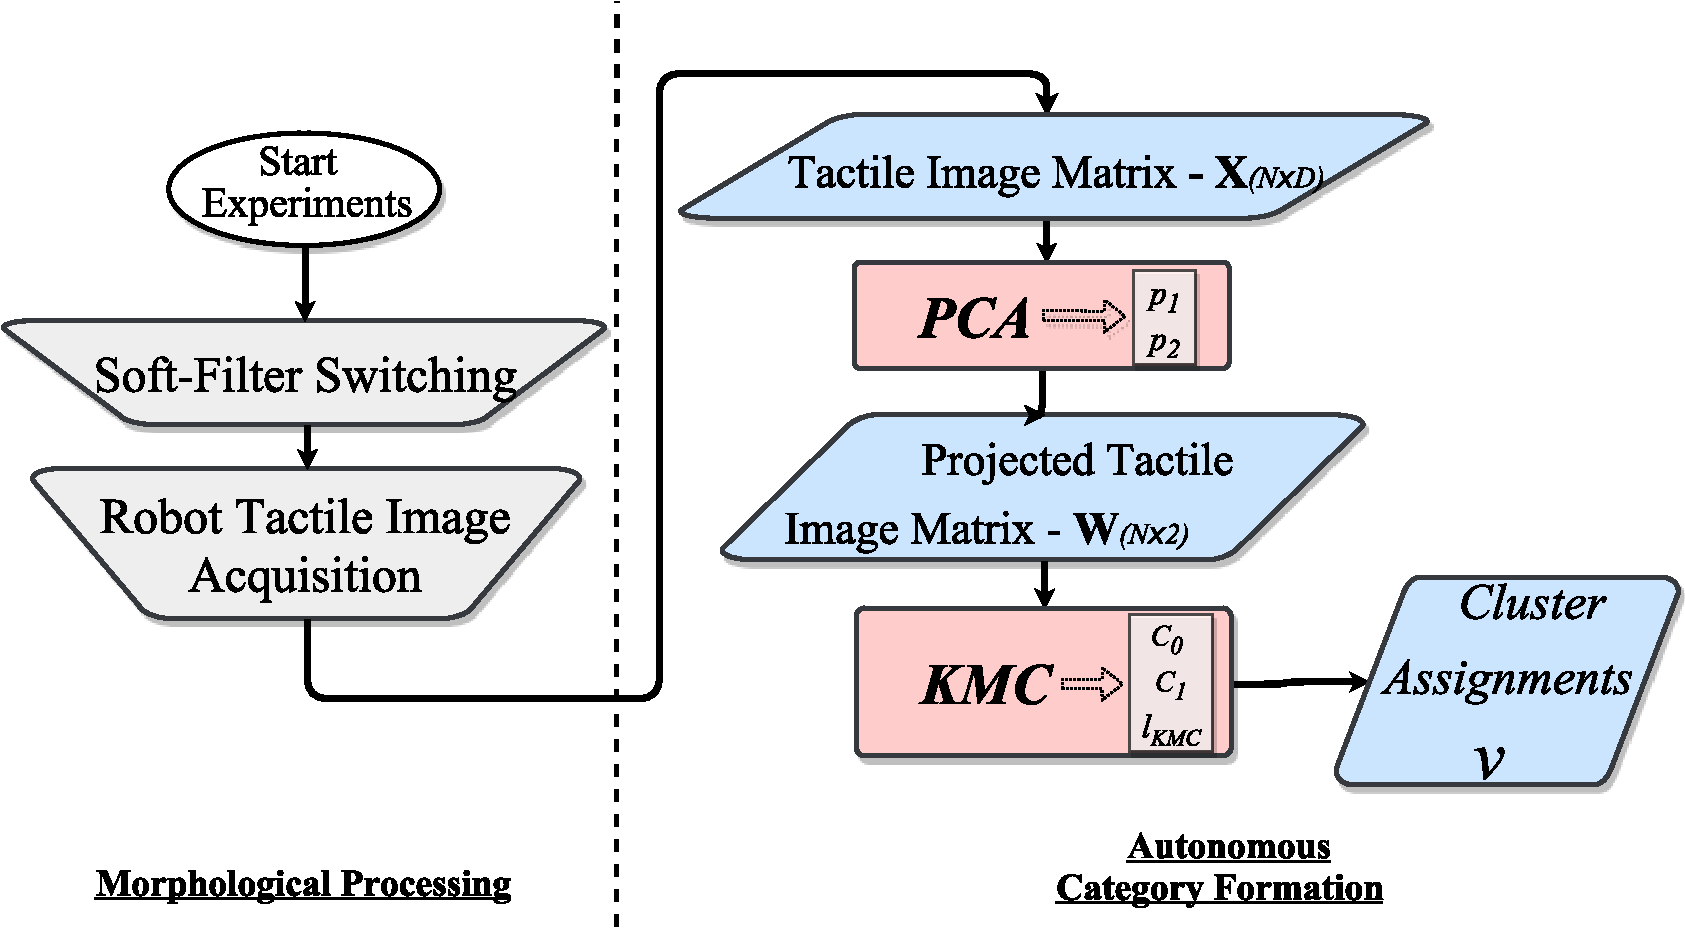
\includegraphics[width=.45\textwidth]{./figs/clustering_process.pdf}
	\caption{Autonomous category formation steps.} %{After acquiring morphologically processed $tactile\ images$ for each object in a set, the high dimensional images are first projected in a 2-dimensional subspace ($PCA$) and finally clustered in an unsupervised manner through the $KMC$ algorithm. After clustering, $v$ is vector containing the cluster membership of each object in the initial set.}%}
	\label{self_org_processing}
	\vspace{8pt}
\end{figure}
We propose an unsupervised process to automatically cluster a set of objects in two categories. After acquiring tactile images for each object in a set, the autonomous category formation process is mainly divided in two pipelined steps: Principal Component Analysis projection ($PCA$) \cite{tipping_probabilistic_1999} and K-Means Clustering ($KMC$) \cite{lloyd_least_1982}. We use the proposed process to observe the influence soft filters with variable thickness have on the categories.

We start the process with tactile sensor readings for each object we wish to cluster. For a set of $N$ different objects, let $\mathbf{X}$ be a $(N\times D)$ matrix where each unique tactile \emph{image} for an object is a $D$  dimensional row ($D\gg2$) in the matrix. We define a tactile image as a one-off tactile sensor reading, where each element in the vector is proportional to the deformation of a tactile element in a predetermined location on the sensor (Fig. \ref{CySkin:skin}). As the tactile sensor technology does not affect the processing stages, we leave its description to Section \ref{sec_setup}. We begin by finding the average tactile image by
\begin{equation}
\vec{\mu} = \frac{1}{n}\sum_{i=1}^{n}\vec{x}_i
\end{equation}
where $\vec{x}_i$ is a row vector in $\mathbf{X}$. We proceed by computing the scatter matrix of $\mathbf{X}$ as
\begin{equation}
\mathbf{S} = \sum_{i=1}^{n}(\vec{x}_i-\vec{\mu})(\vec{x}_i-\vec{\mu})^T
\end{equation}
We use Single Value Decomposition to factorize $\mathbf{S}$ into
\begin{equation}
\mathbf{S} = \mathbf{Q}\mathbf{\Lambda} \mathbf{Q}^{-1}
\end{equation}
\noindent where $\mathbf{Q}$ is matrix such that each column $q_j$ corresponds to an eigenvector of $\mathbf{S}$, and each element $\lambda_{jj}$ in the diagonal matrix $\Lambda$ is its corresponding eigenvalue. 
\begin{figure}[]
	\centering
	\begin{subfigure}[b]{.27\textwidth}
		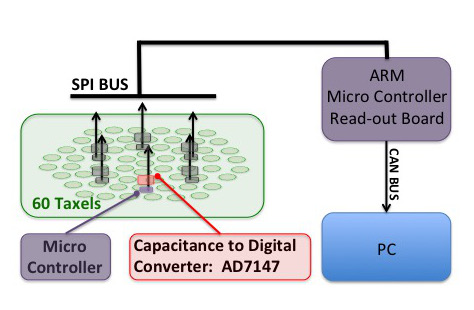
\includegraphics[width=\textwidth]{./figs/CySkin.jpg}
		\caption{}
		\label{CySkin:schema}
	\end{subfigure} 
	\hspace{0.01\textwidth}
	\begin{subfigure}[b]{0.18\textwidth}
		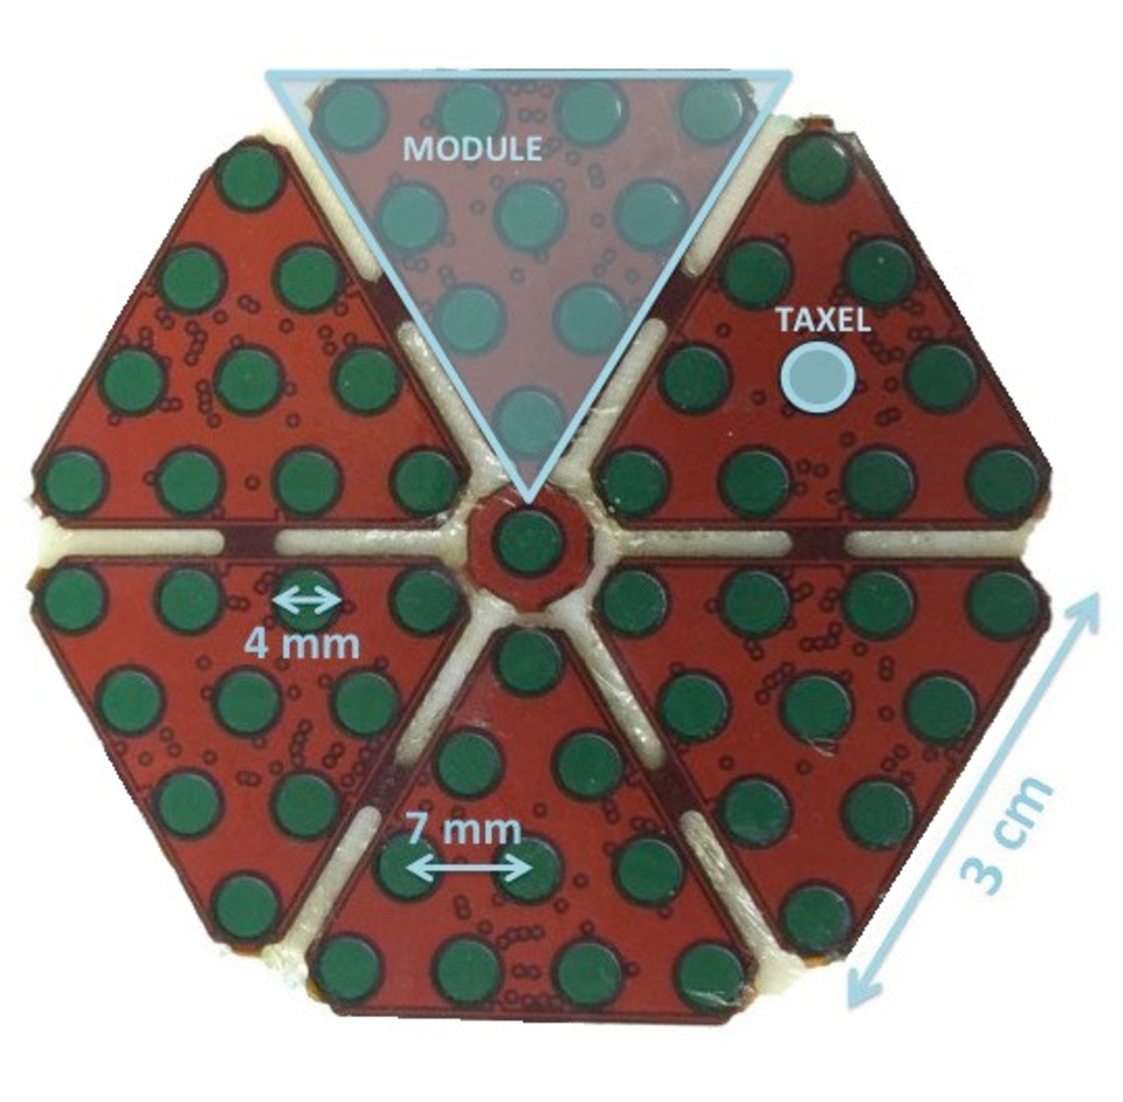
\includegraphics[width=\textwidth]{./figs/skin_sensor.pdf}
		\caption{}
		\label{CySkin:skin}
	\end{subfigure}
	\caption{(a) The CySkin technology architecture. The hexagonal patch is connected to a Intelligent Hub Board (IHB) that collect the tactile sensor data and send them to the PC through a CAN bus. (b) The CySkin patch used for the experiments. It is composed by 6 interconnected triangular modules, each hosting 10 taxels.}
	\label{CySkin}
	\vspace{10pt}
\end{figure}
We list the eigenvectors in ascending order of eigenvalue and select the first two in the list. Let $\vec{p}_1$ and $\vec{p}_2$ be the selected eigenvectors obtained from $PCA$. We form a $(D\times 2)$ projection matrix 
\begin{equation}
\mathbf{P}=\begin{bmatrix}\vec{p}_1^{\ T}, \vec{p}_2^{\ T}\end{bmatrix}	
\end{equation}
where $\vec{p}_1^{\ T}$ and $\vec{p}_2^{\ T}$ are column vectors in $\mathbf{P}$. Finally, we project the $D$-dimensional row vectors in $\mathbf{X}$ onto a 2-dimensional subspace by:
\begin{equation}
\mathbf{W}=\mathbf{X}\cdot \mathbf{P}
\end{equation}
where $\mathbf{W}$ is a $(N\times 2)$ matrix and each row in it is a 2-dimensional $encoding$ of a tactile image. We proceed by using $KMC$ (k=2 and random centroid initialization) to split the tactile images in $\mathbf{W}$ into two clusters, thus:
\begin{equation} \label{kmc_eq}
\vec{v} = KMC_{k=2}(\mathbf{W})
\end{equation}
where $\vec{v}$ is an N-dimensional array, $\forall i\in \{1, 2,\ ...\ , N\}$.   $\vec{v}_i\in\{0,1\}$, and $\forall i\ \exists j.\ i\neq j\ \land\ v_i\neq v_j$ (no one cluster can contain all objects). In general $\vec{v}_i=0\ iff$ the $i^{th}$ tactile image belongs to cluster 0 and $\vec{v}_i=1\ iff$ the $i^{th}$ tactile image belongs to cluster 1 (Fig. \ref{self_org_processing}). The $\vec{v}$ vector then contains the cluster membership of each object in the initial set. To avoid cluster anomalies due to the random centroid initializations we run the K-Means Clustering algorithm three times and discard the clustering attempt if, after convergence, any of the three cluster guesses vectors differs from any other.
 
As it becomes clearer later, the cluster assignments for each object are largely dependent on the soft filter employed. The change in cluster assignment is the main object of analysis in the following sections.



\section{Methods and Experimental Set-Up}\label{sec_setup}
\begin{figure}[]
	\centering
	\begin{subfigure}[b]{0.45\textwidth}
		\includegraphics[width=\textwidth]{./figs/set_up.pdf}
	\end{subfigure} 
	\caption{The experimental set-up used for the experiments. The ST robot was used to push the sensorised end-effector against the object. A FlexiForce sensor A502 from TekScan was used for controlling the normal force applied. Three different soft filters were used in the experiments}
	\label{setup}
	\vspace{8pt}
\end{figure}
We investigate the influence soft filters with varying thickness have on tactile information encoding. We build three filters using Ecoflex 00-20\footnote[2]{https://www.smooth-on.com/products/ecoflex-00-20/} from Smooth-on, each respectively $3mm$, $6mm$ and $10mm$ thick. The material was selected for its mechanical properties, in particular a Shore Hardness of 00-22.
We 3D-print a custom-made end-effector with a circular flat surface ($diameter=80mm$) onto which the soft filters can later be placed and we integrate a capacitive tactile sensor onto its surface to retrieve tactile images of the objects during the experiments (the above set up is described in Fig. \ref{setup}).
The reference tactile sensor technology has been described in \cite{schmitz_methods_2011}. The adopted sensing mode is based on the capacitive transduction principle. A capacitive transducer (i.e., a tactile element, or taxel) is organized in a layered structure: the lower layer consists of the positive electrode, which is mounted on a Flexible Printed Circuit Board (FPCB); a small air chamber act as dielectric and the upper layer is a ground plane made with conductive lycra. The tactile sensor is made up of a number of taxels geometrically organized in triangular modules (Fig. \ref{CySkin:skin}). 
In the current prototype, each module hosts $10$ taxels, as well as the Capacitance to Digital Converter (CDC) chip (namely, the AD7147 from Analog Devices) for converting capacitance values to digital. The CDC chip can measure variations in capacitance values with 16 bits of resolution. All the modules are interconnected and communicate through an SPI bus to a read-out board which perform a preliminary processing of the tactile sensor data and send them to the PC through CAN bus (Fig. \ref{CySkin:schema}). %within the $4 \div 30pF$ range with a sensitivity of $0.32fF$. 
In this context, the normal forces exerted on the sensor produce variations in capacitance values reflecting the varied pressure over the taxel positions.  A sensor reading from the tactile sensor described is produced at $20Hz$, and corresponds to a 60-dimensional array (we exclude the central taxel in Fig. \ref{CySkin:skin}), where each element contains the capacitance variation value of the corresponding taxel.
%is $\Delta C_i$, and $i$ is its corresponding taxel in the sensor.
In this paper we refer to tactile images as the sensor readings for a specific object.
To carry out the experiments we design and 3d-print a minimalistic set of four different objects with distinct features: a Cube ($side=30mm$), a Cuboid ($side=30mm$, $length=80mm$), a Sphere ($radius=30mm$) and a Half-Cylinder ($radius=30mm$, $length=80mm$). The objects present mainly two varying properties: long vs short length (Sphere \& Cube vs Half-Cylinder \& Cuboid) and edged vs non-edged surfaces (Cube \& Cuboid vs Sphere \& Half-Sphere). We define a task as a unique split of objects into two sets. Given the 4 objects it follows we can derive 7 different tasks (Fig. \ref{task_table}). A task here represents one of the possible ways we could wish to perceive similarities among objects. If we were to cluster objects according to Task 5, for example, we would be associating objects based on edges; while optimizing for Task 6 would signify grouping objects by length. Some of the tasks are conceptually less intuitive as no one particular feature can resolve the inclusion of an object in a cluster. As we are interested in the effects of morphological processing to the objects' associations, all 7 tasks are considered.
\begin{figure}[]
	\centering
	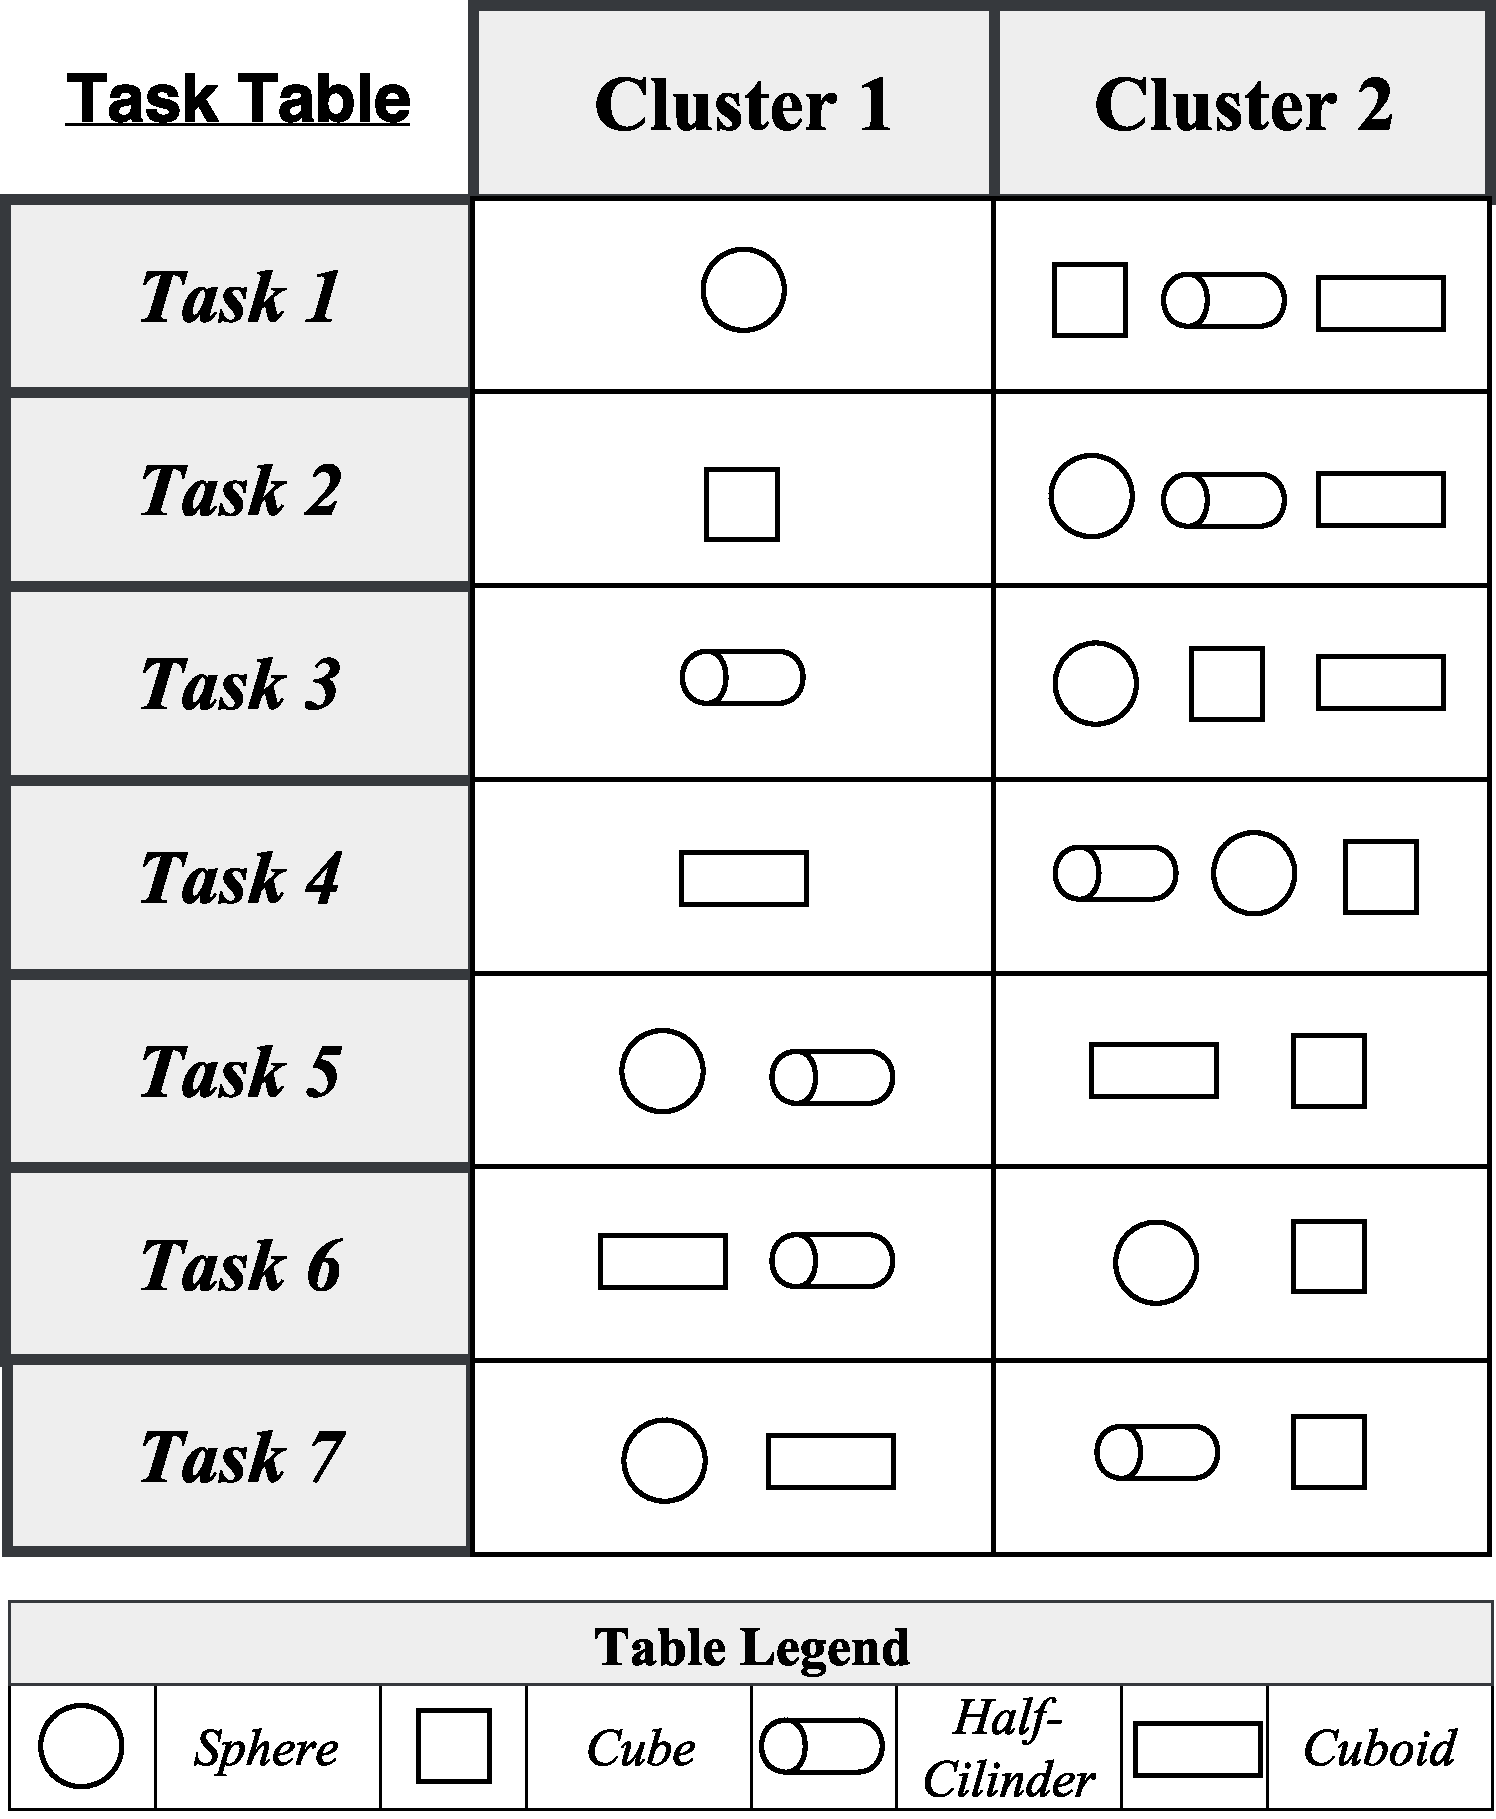
\includegraphics[width=.36\textwidth]{./figs/TaskTable.pdf}
	\caption{Task Table. Each task is a possible clustering outcome for the object set.}
	\label{task_table}
\end{figure}
We carry out the experiments by mounting the printed end-effector, coupled with the tactile sensor, onto an ST-Robotics R12/5 robotic arm\footnote[3]{http://www.robotshop.com/uk/st-robotics-r12-5-axis-articulated-robot-arm.html}. For each set of experiments we secure a different soft filter onto the end-effector flat's surface, and proceed by controlling the arm to descend perpendicularly down on the center of the object (Fig. \ref{setup}). 
We place a FlexiForce force sensor A502\footnote[4]{https://www.tekscan.com/products-solutions/force-sensors/a502} at the base of the object in order to apply a controlled perpendicular force when retrieving tactile images. The linear range of the sensor is 0-22N, however, we recalibrate its response in the 0-10N range and choose the maximal calibrated force of 10N, as this falls in the low-pressure regime (characterized as gentle touch \cite{dellon1992human}) for object exploration. We arrest the arm for the time needed to retrieve 10 consecutive tactile sensor readings and average them to create a tactile image. To further remove experimental bias, we repeat each set of experiments three times and average the computed tactile images, for each object, over the three trials (Fig. \ref{parts}). We finally construct the tactile image matrix $\mathbf{X}$ by setting each of its rows to a computed tactile image.
We utilize the process described in Section \ref{sec_unsup_clustering} to process the tactile image matrix for each experiment. 
\begin{figure}[]
	\flushleft
	\begin{subfigure}[b]{0.465\textwidth}	
		\begin{subfigure}[b]{0.04\textwidth}
			
\includegraphics[width=\textwidth]{./figs/blank_label.jpg}
		\end{subfigure}
		\begin{subfigure}[b]{.98\textwidth}
			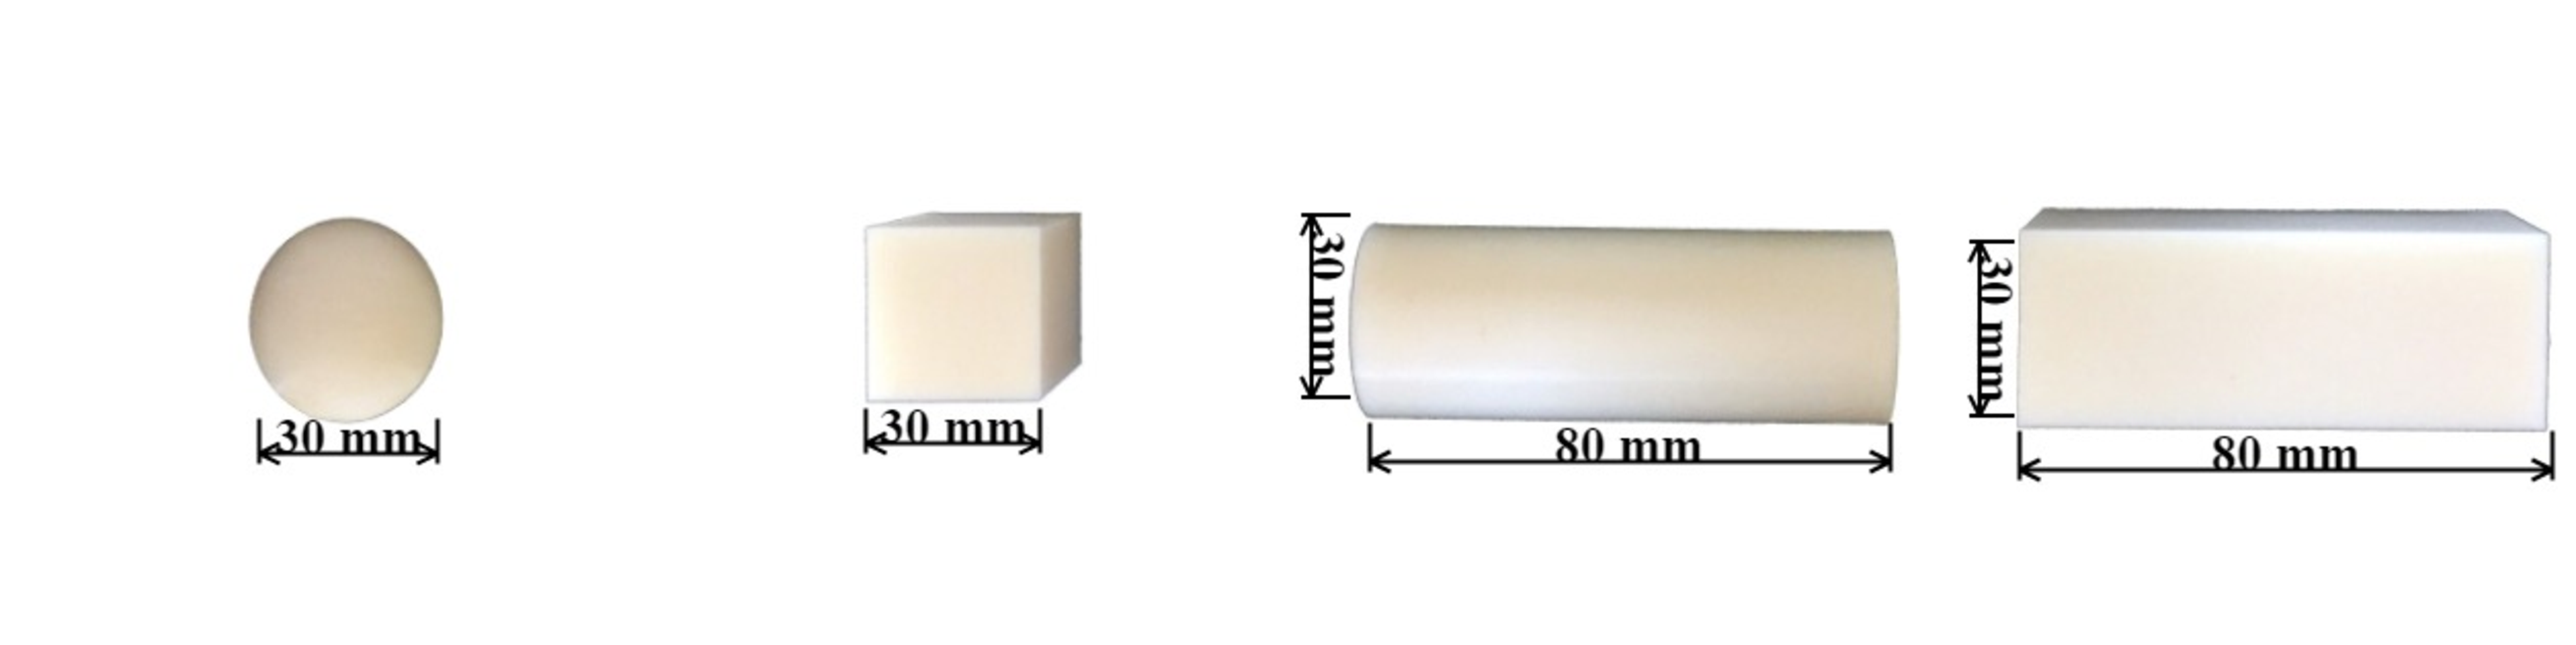
\includegraphics[width=\textwidth]{./figs/objects.pdf}
		\end{subfigure}
	\end{subfigure}\\
	\begin{subfigure}[b]{0.48\textwidth}
		\begin{subfigure}[b]{\textwidth}
			\begin{subfigure}[b]{0.04\textwidth}
				
\includegraphics[width=\textwidth]{./figs/3mil_label.jpg}
			\end{subfigure}
			\begin{subfigure}[b]{0.23\textwidth}
				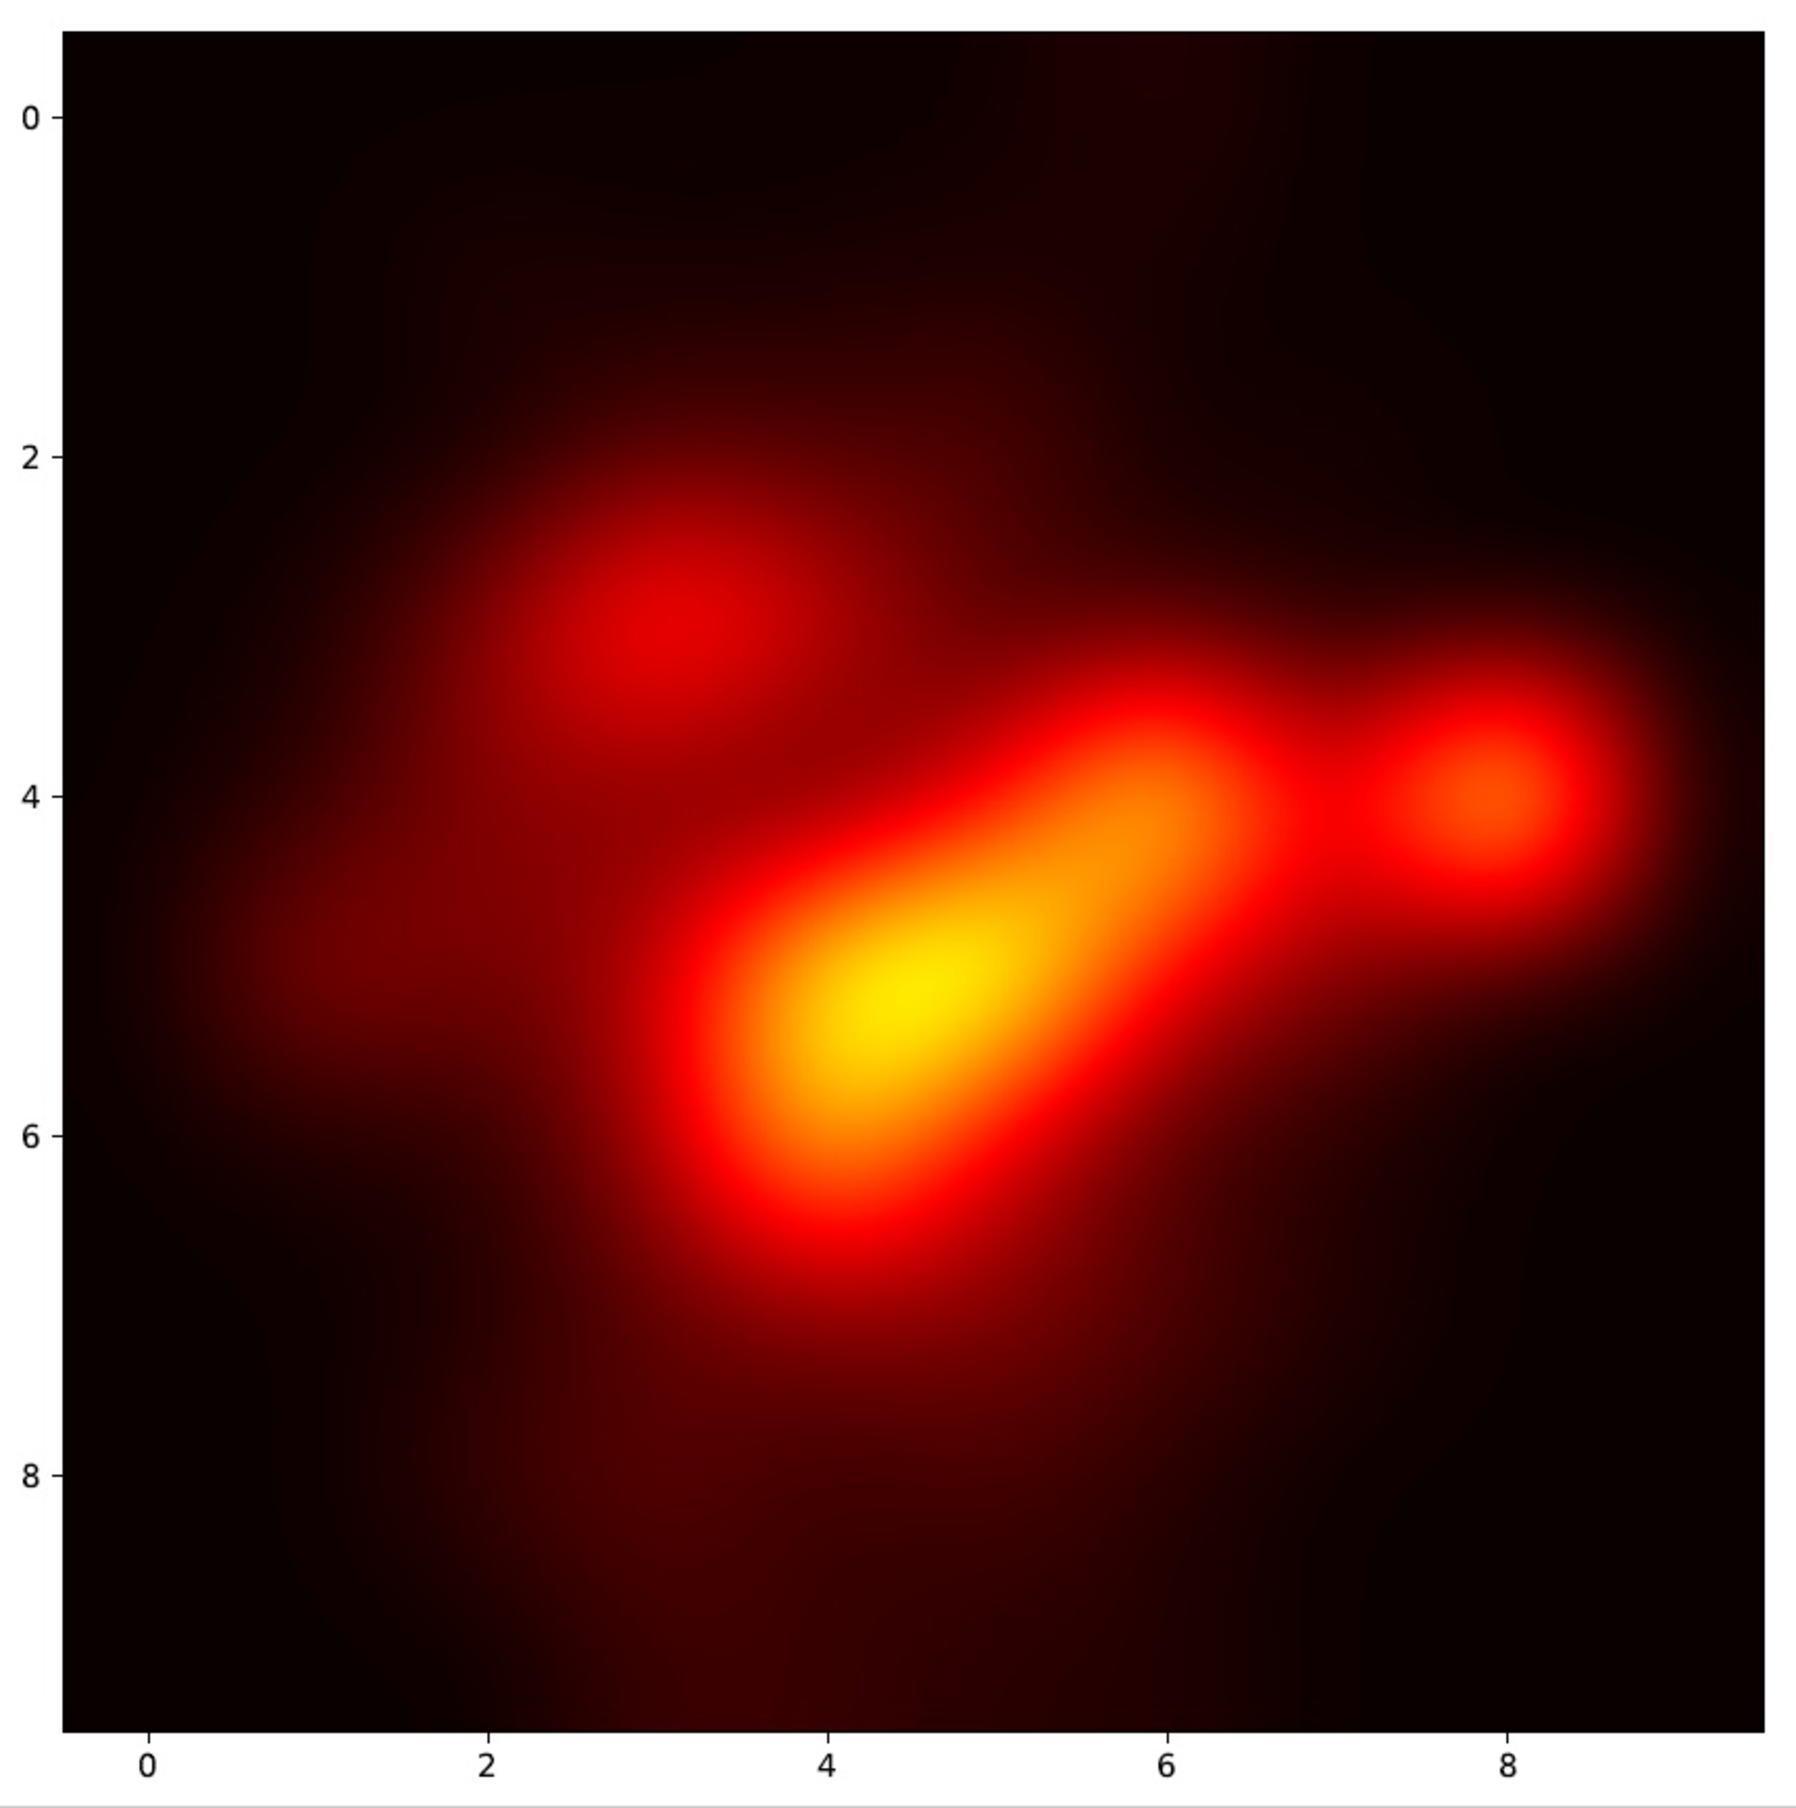
\includegraphics[width=\textwidth]{./figs/3mil_Sphere.pdf}
			\end{subfigure}
			\vspace{-0.9em} % donno why this here words, but it does
			\begin{subfigure}[b]{0.23\textwidth}
				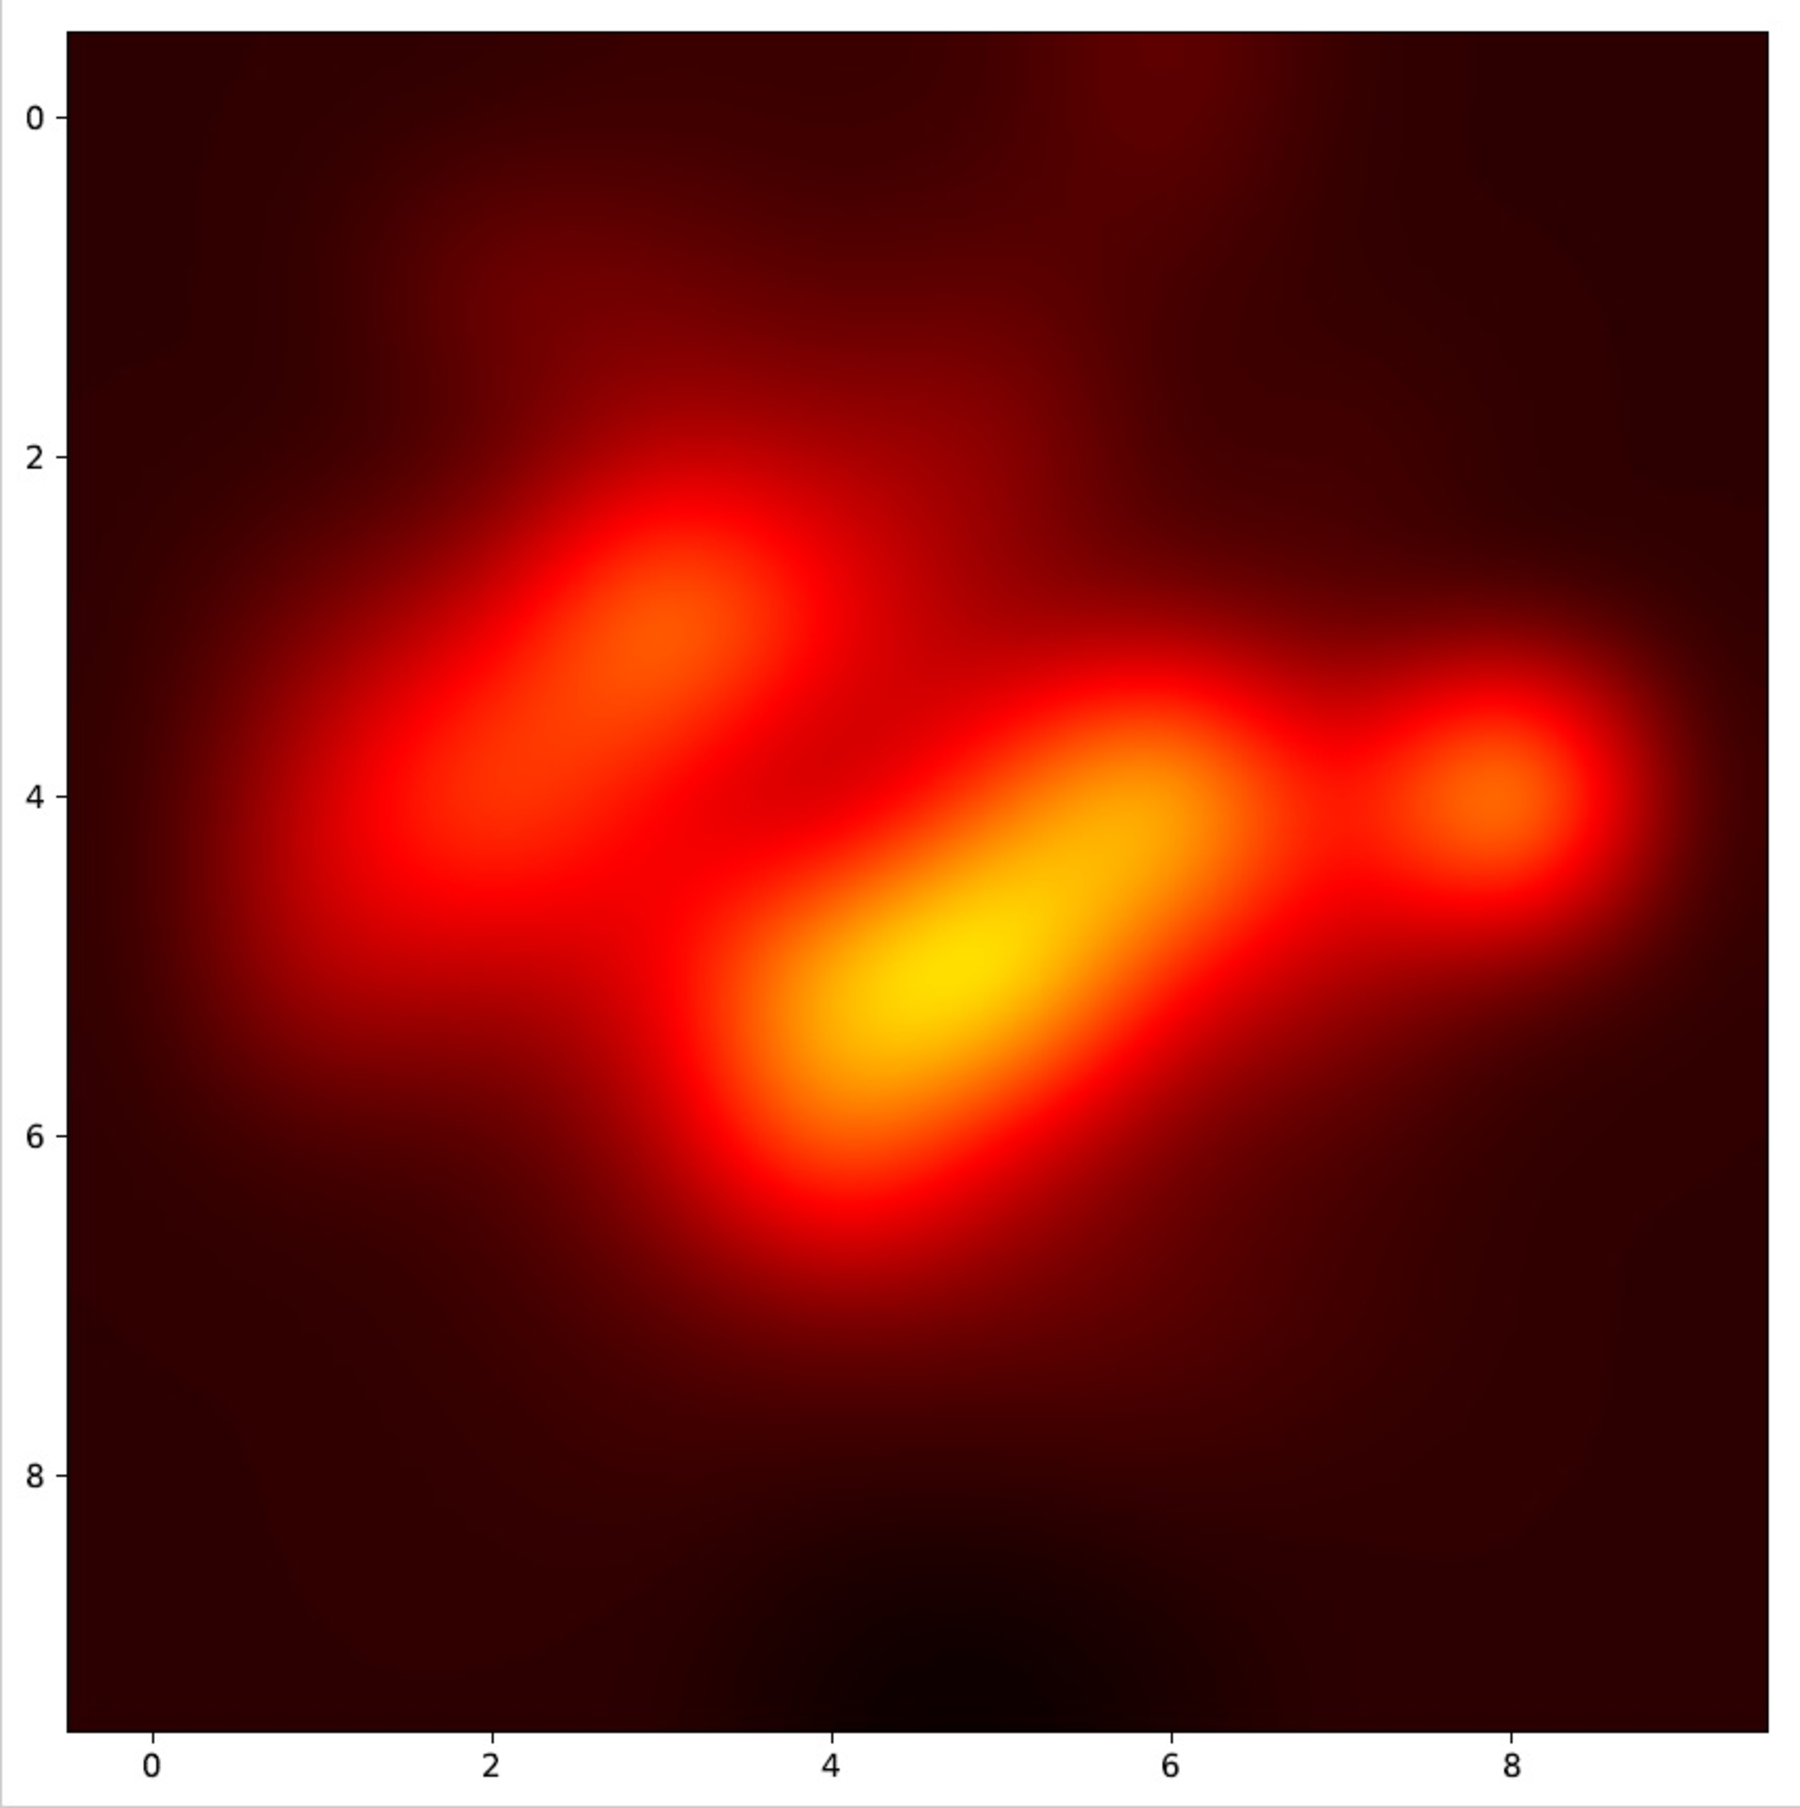
\includegraphics[width=\textwidth]{./figs/3mil_Cube.pdf}
			\end{subfigure}
			\begin{subfigure}[b]{0.23\textwidth}
				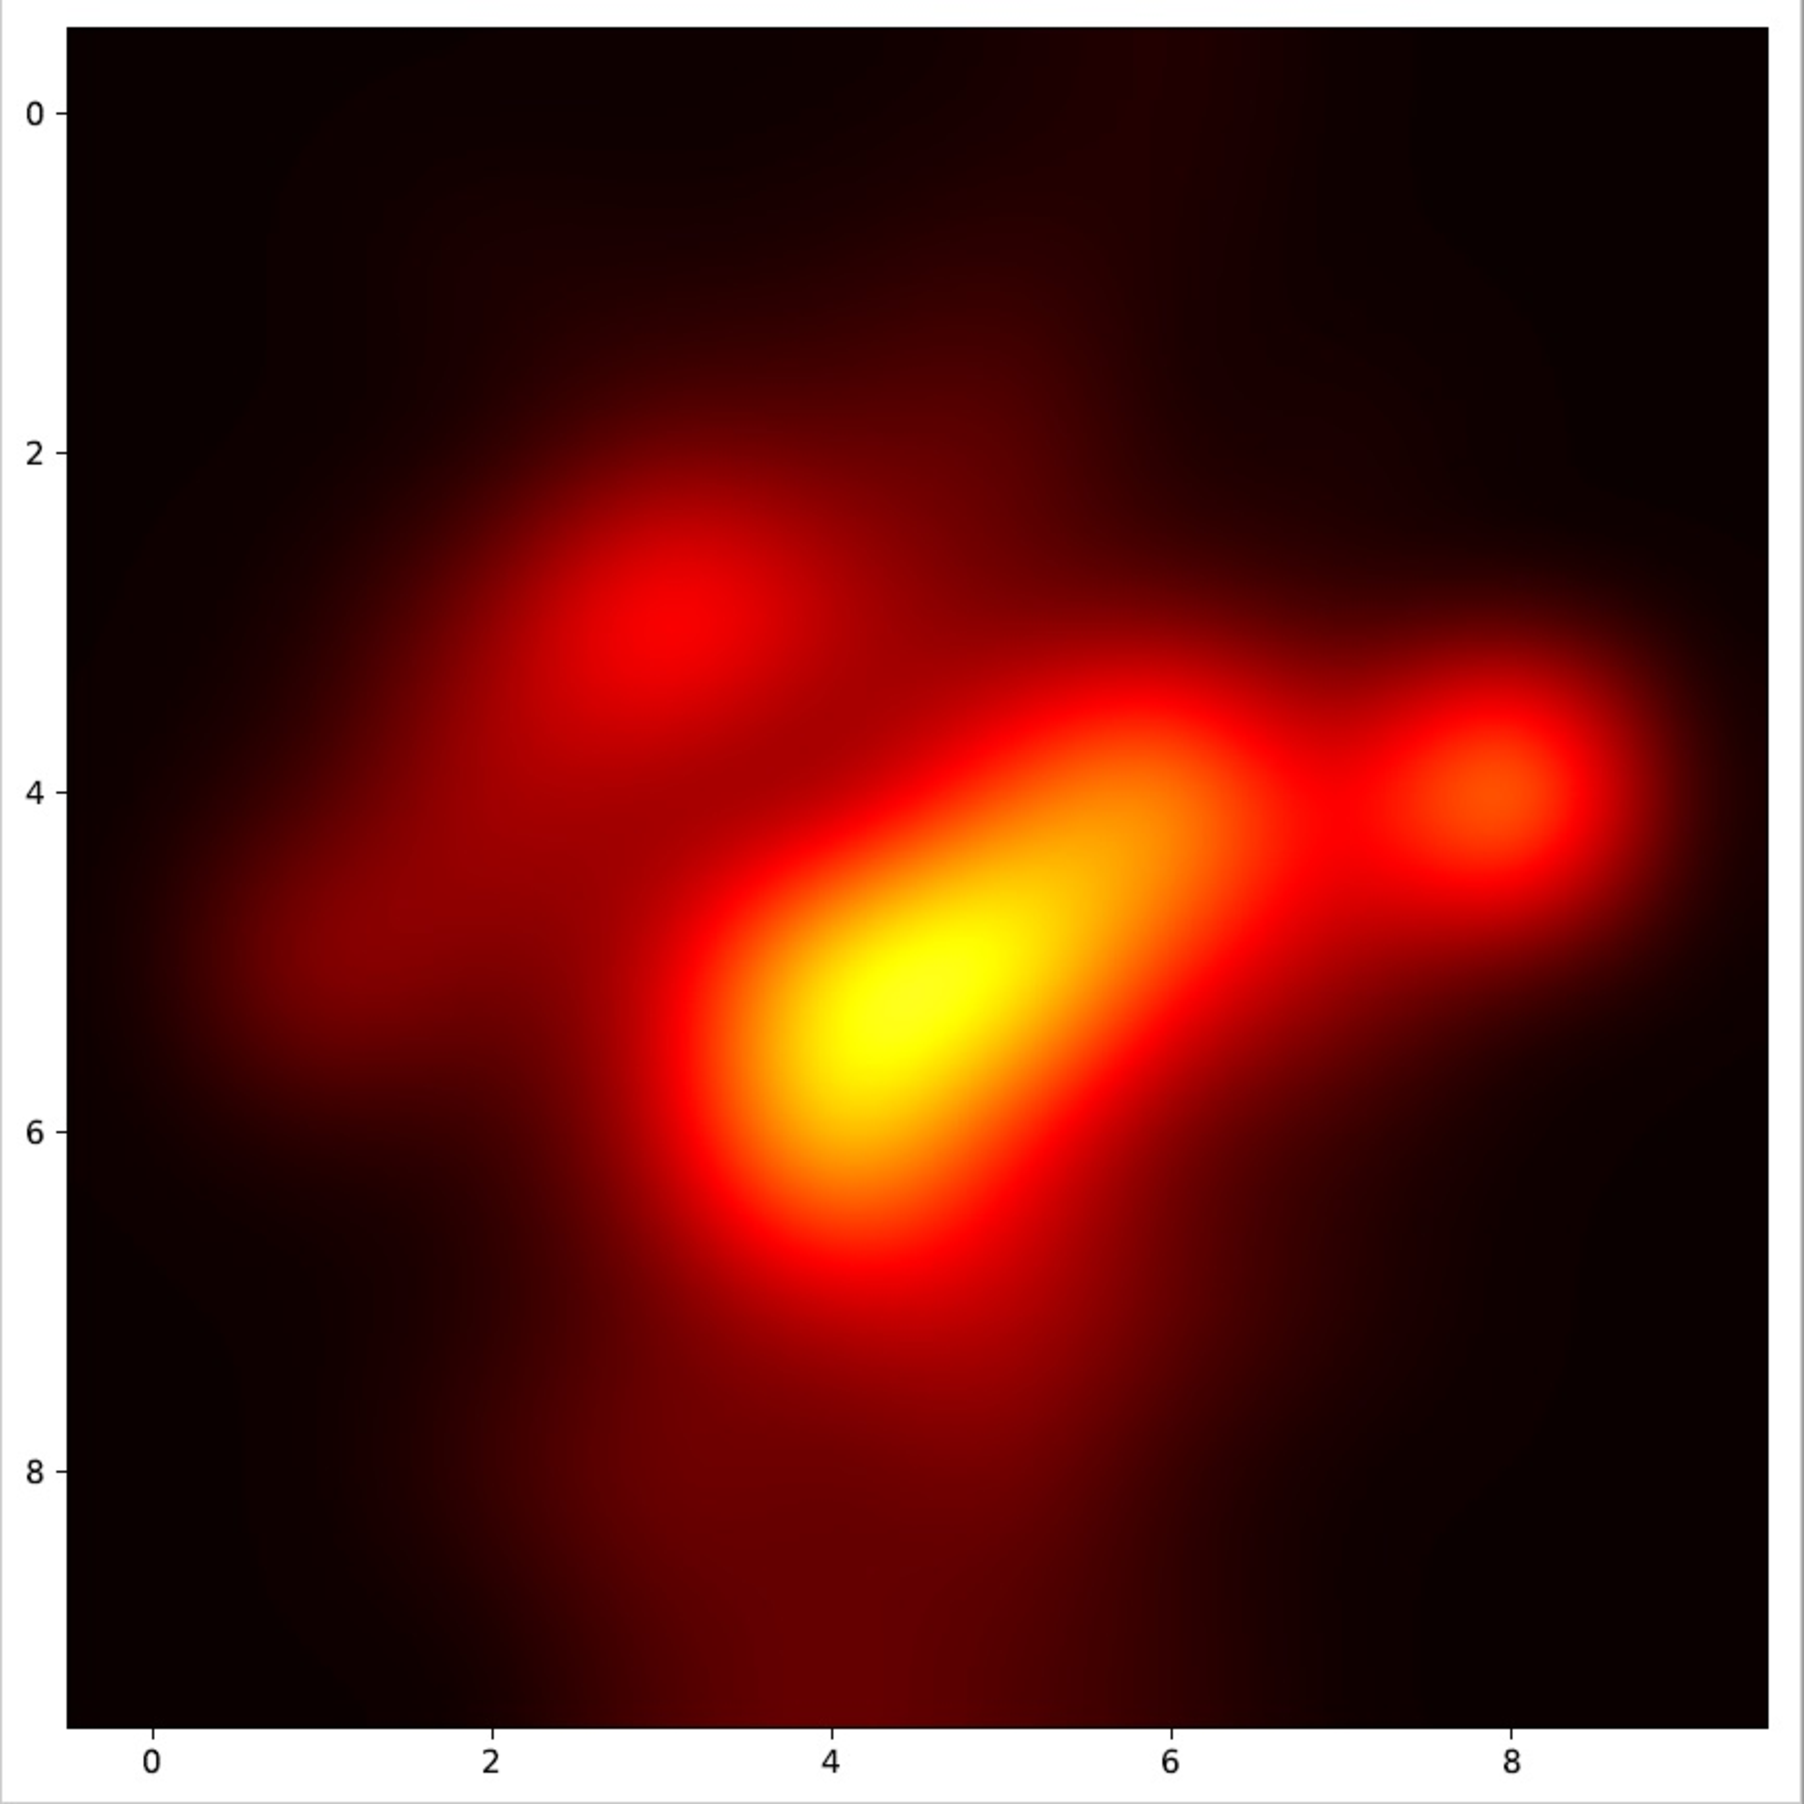
\includegraphics[width=\textwidth]{./figs/3mil_HSphere.pdf}
			\end{subfigure}
			\begin{subfigure}[b]{0.23\textwidth}
				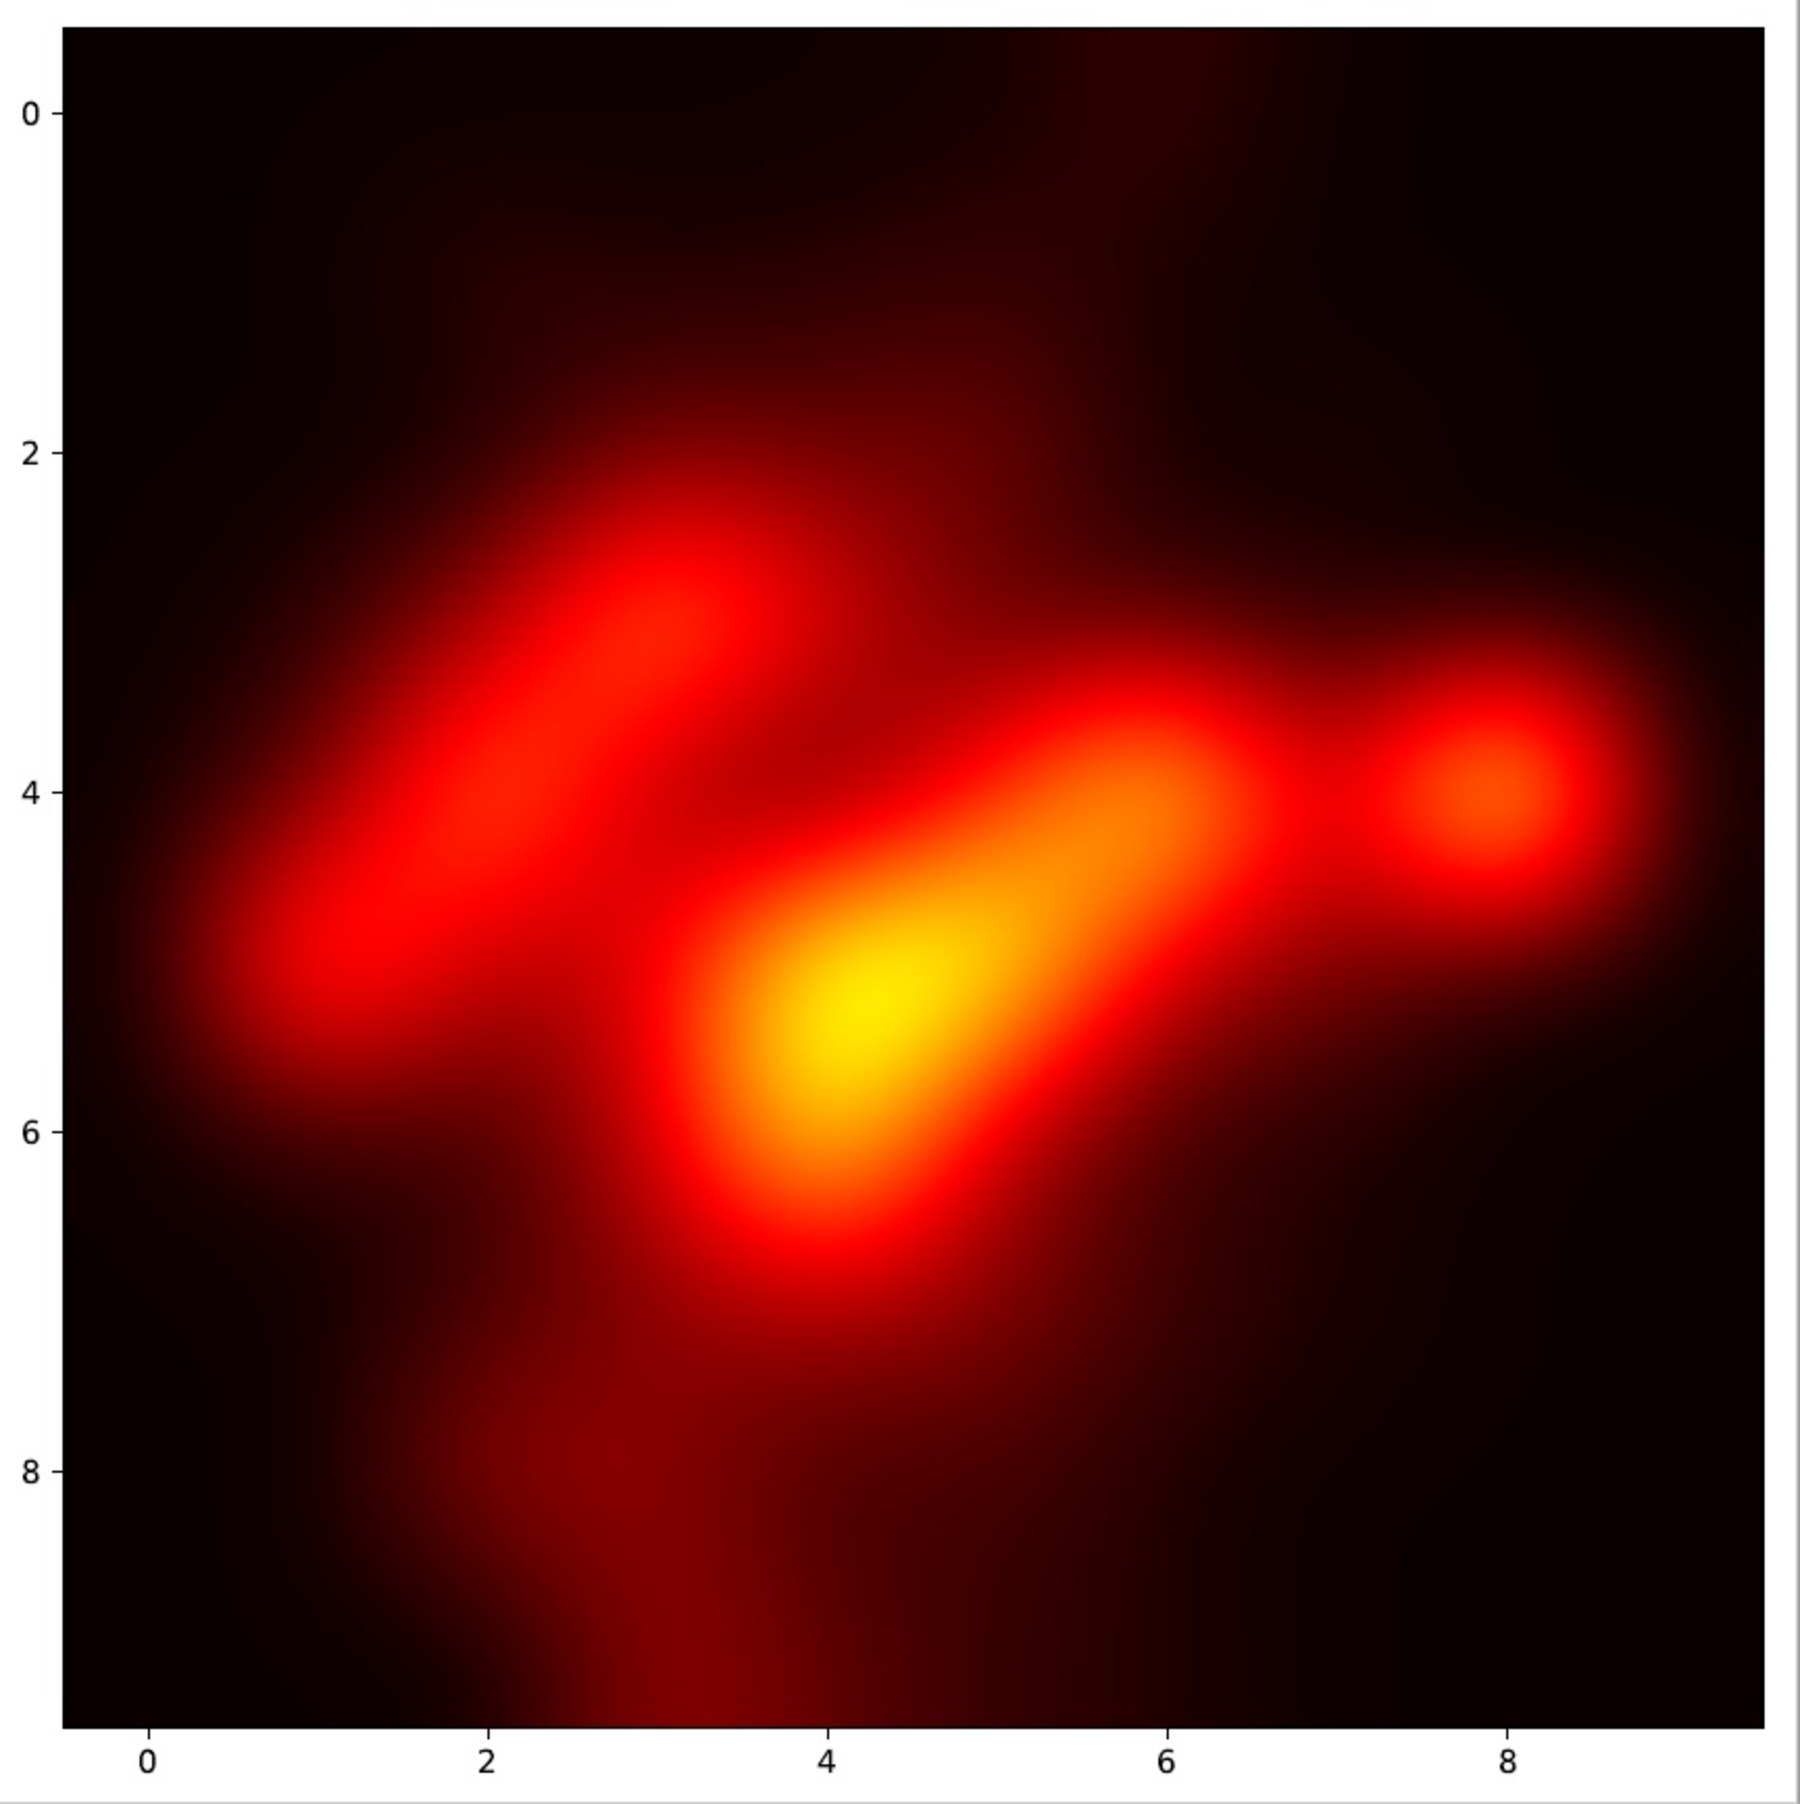
\includegraphics[width=\textwidth]{./figs/3mil_HCube.pdf}
			\end{subfigure}\\
		\end{subfigure}
		\vspace{-0.9em}
		\begin{subfigure}[b]{\textwidth}
			\begin{subfigure}[b]{0.04\textwidth}
				
\includegraphics[width=\textwidth]{./figs/6mil_label.jpg}
			\end{subfigure}
			\begin{subfigure}[b]{0.23\textwidth}
				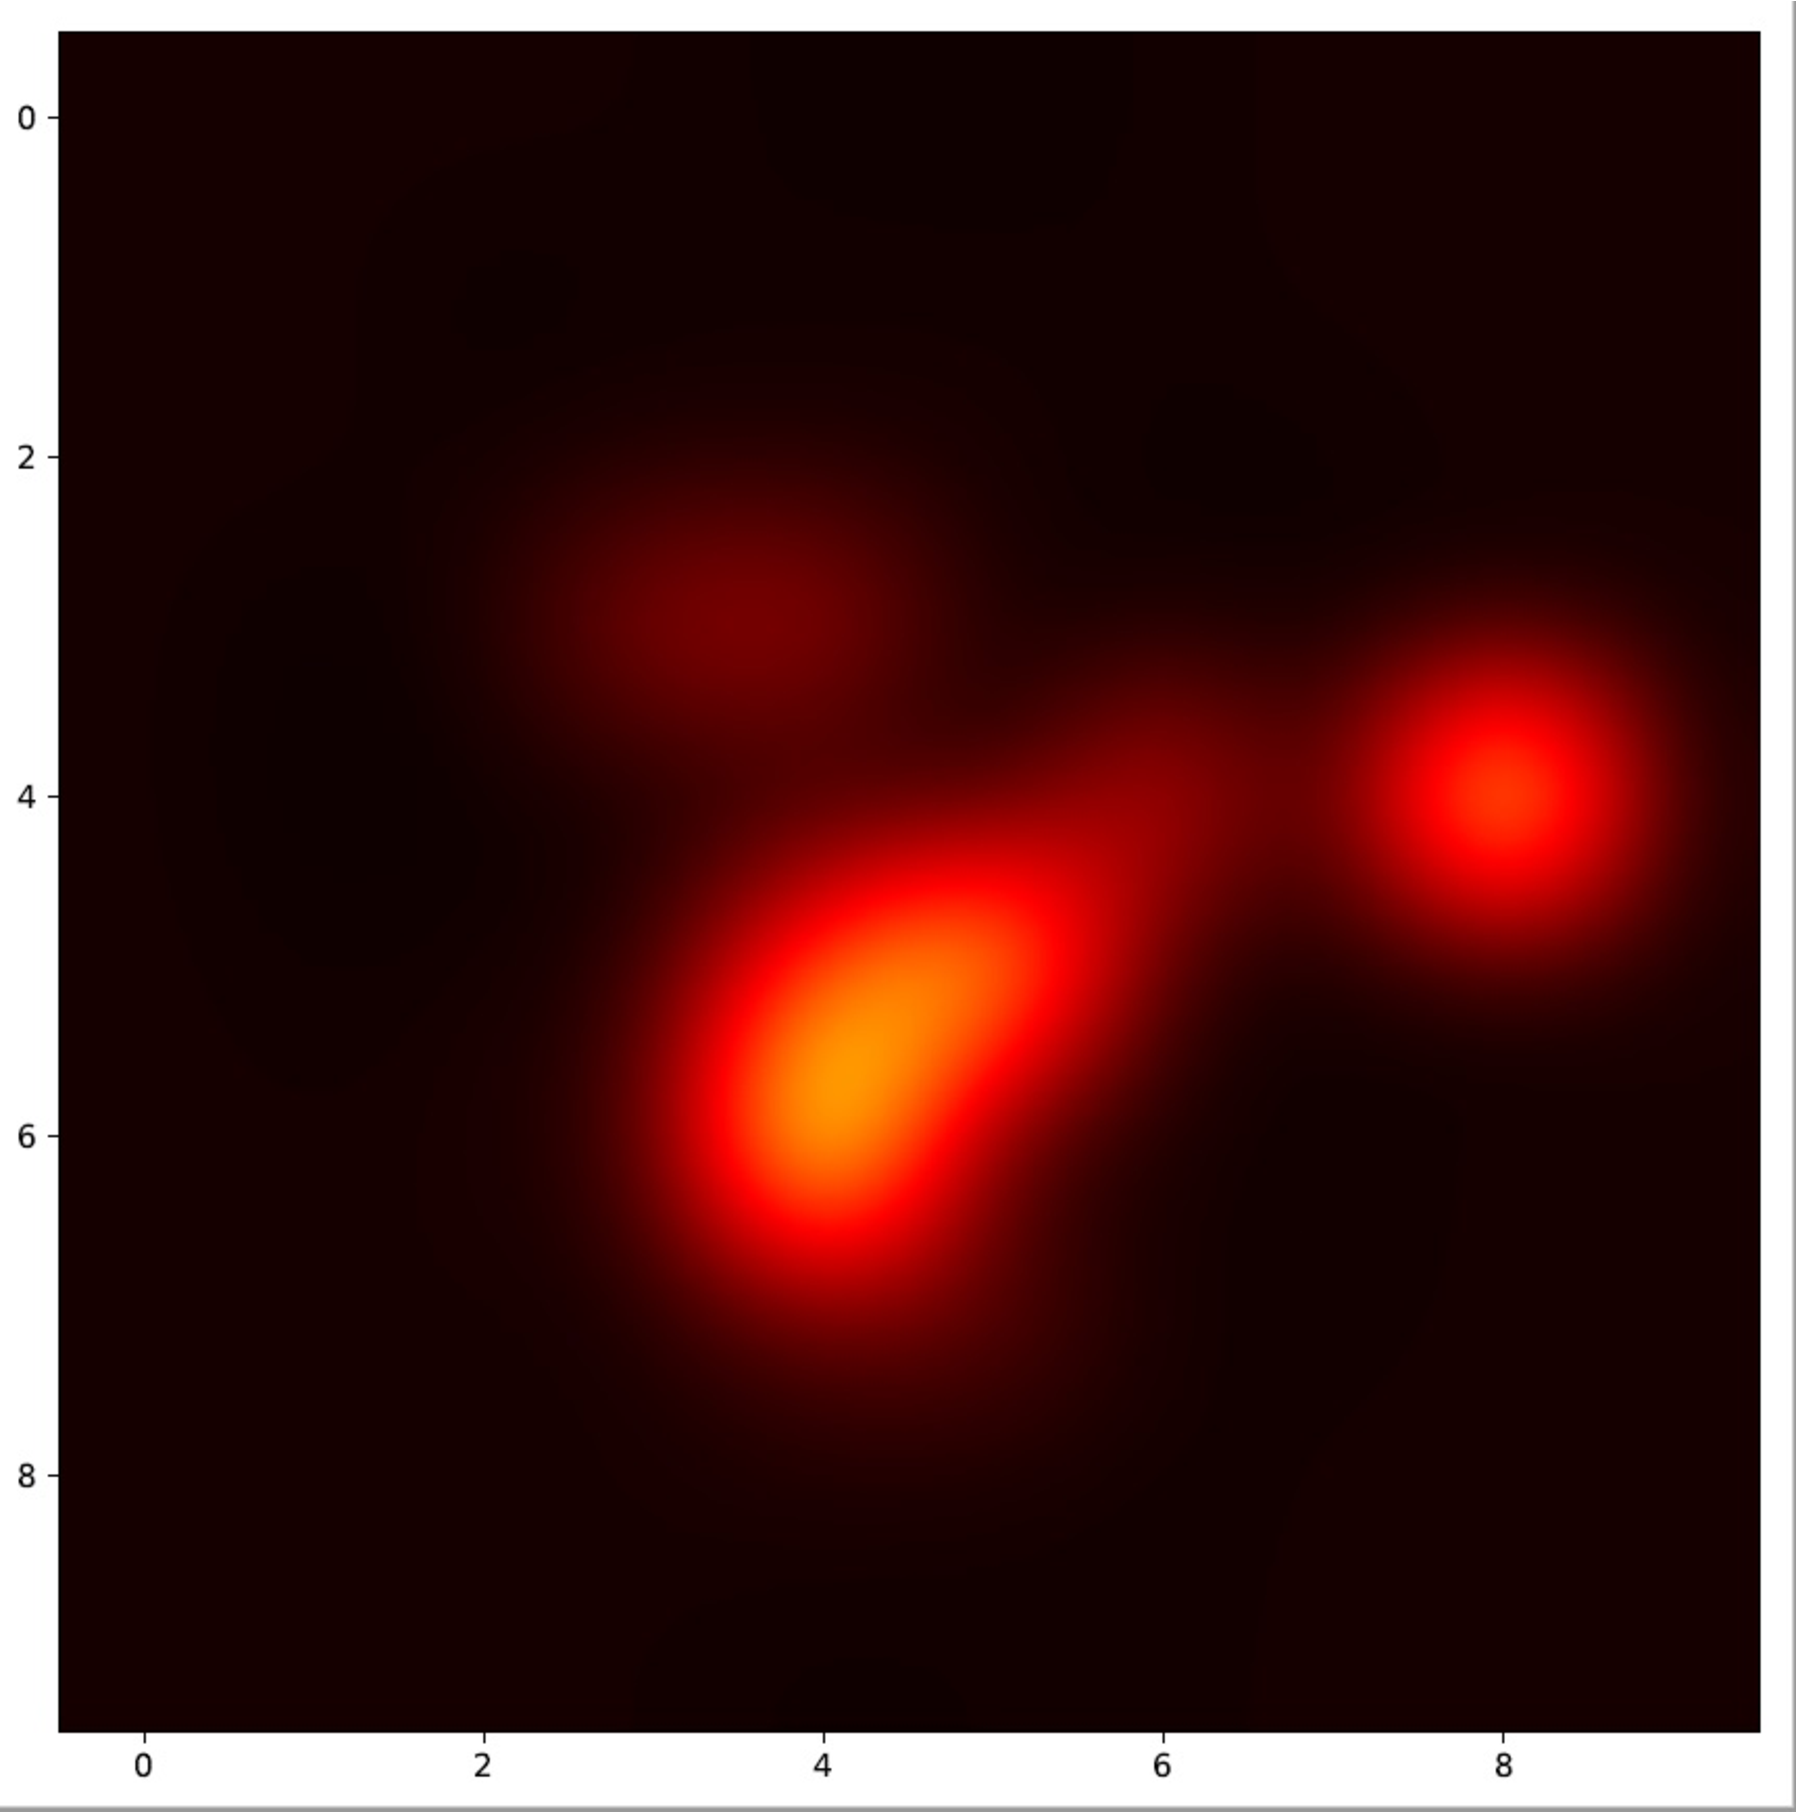
\includegraphics[width=\textwidth]{./figs/6mil_Sphere.pdf}
			\end{subfigure}
			\begin{subfigure}[b]{0.23\textwidth}
				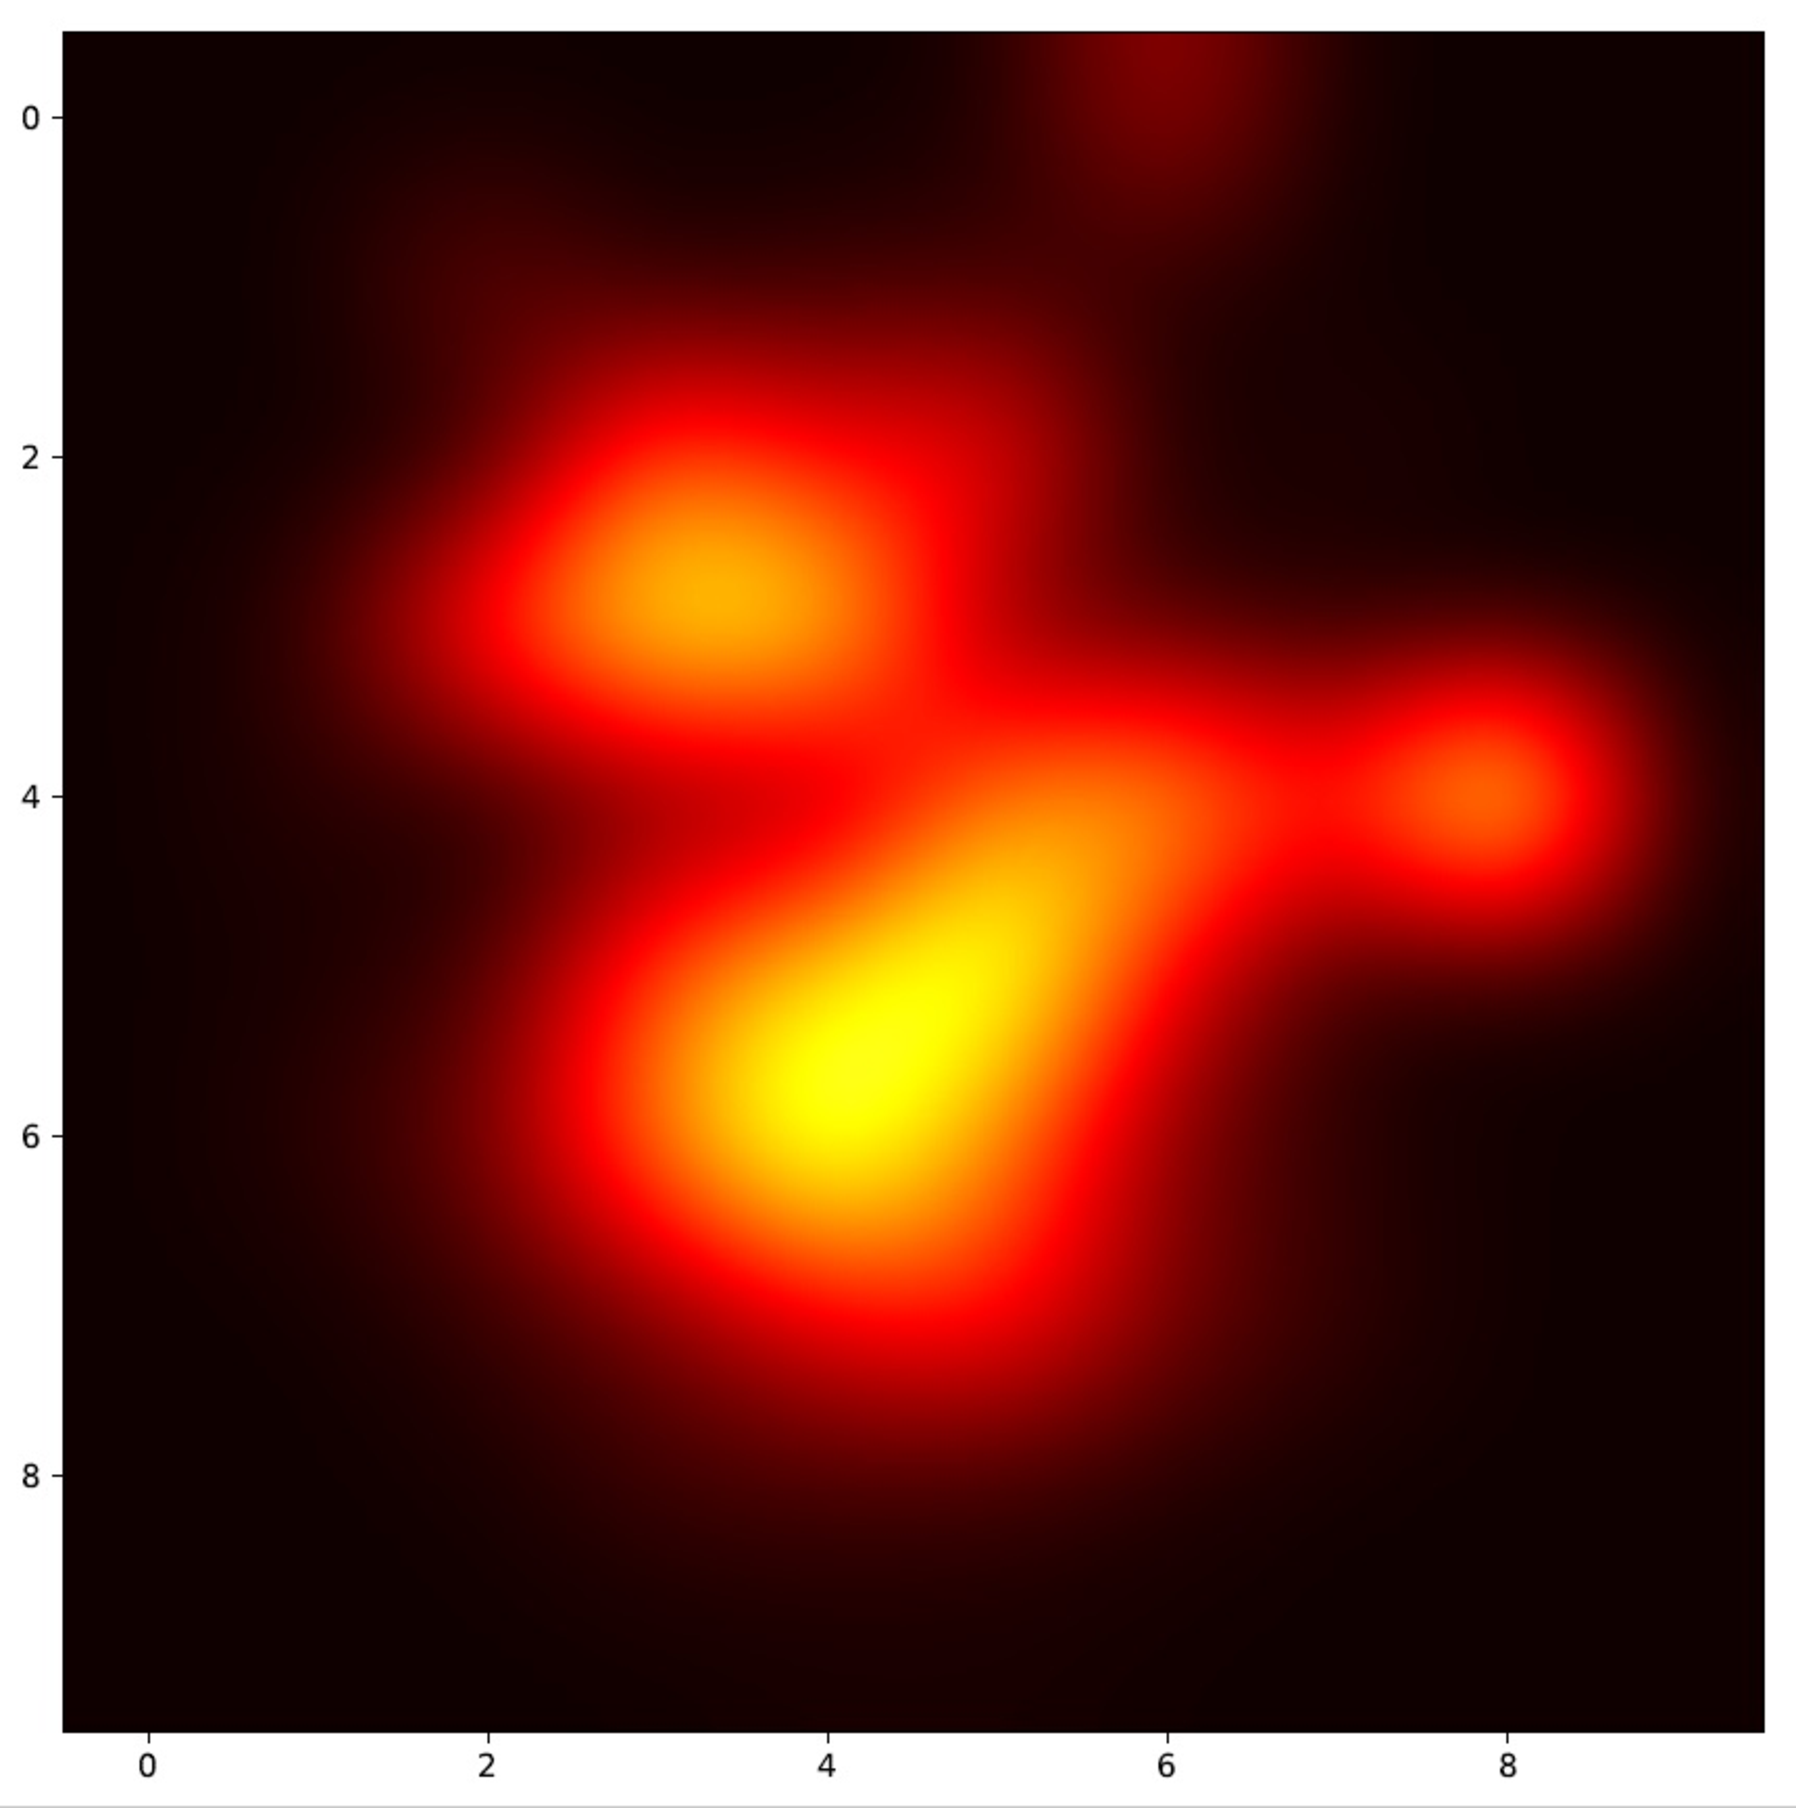
\includegraphics[width=\textwidth]{./figs/6mil_Cube.pdf}
			\end{subfigure}
			\begin{subfigure}[b]{0.23\textwidth}
				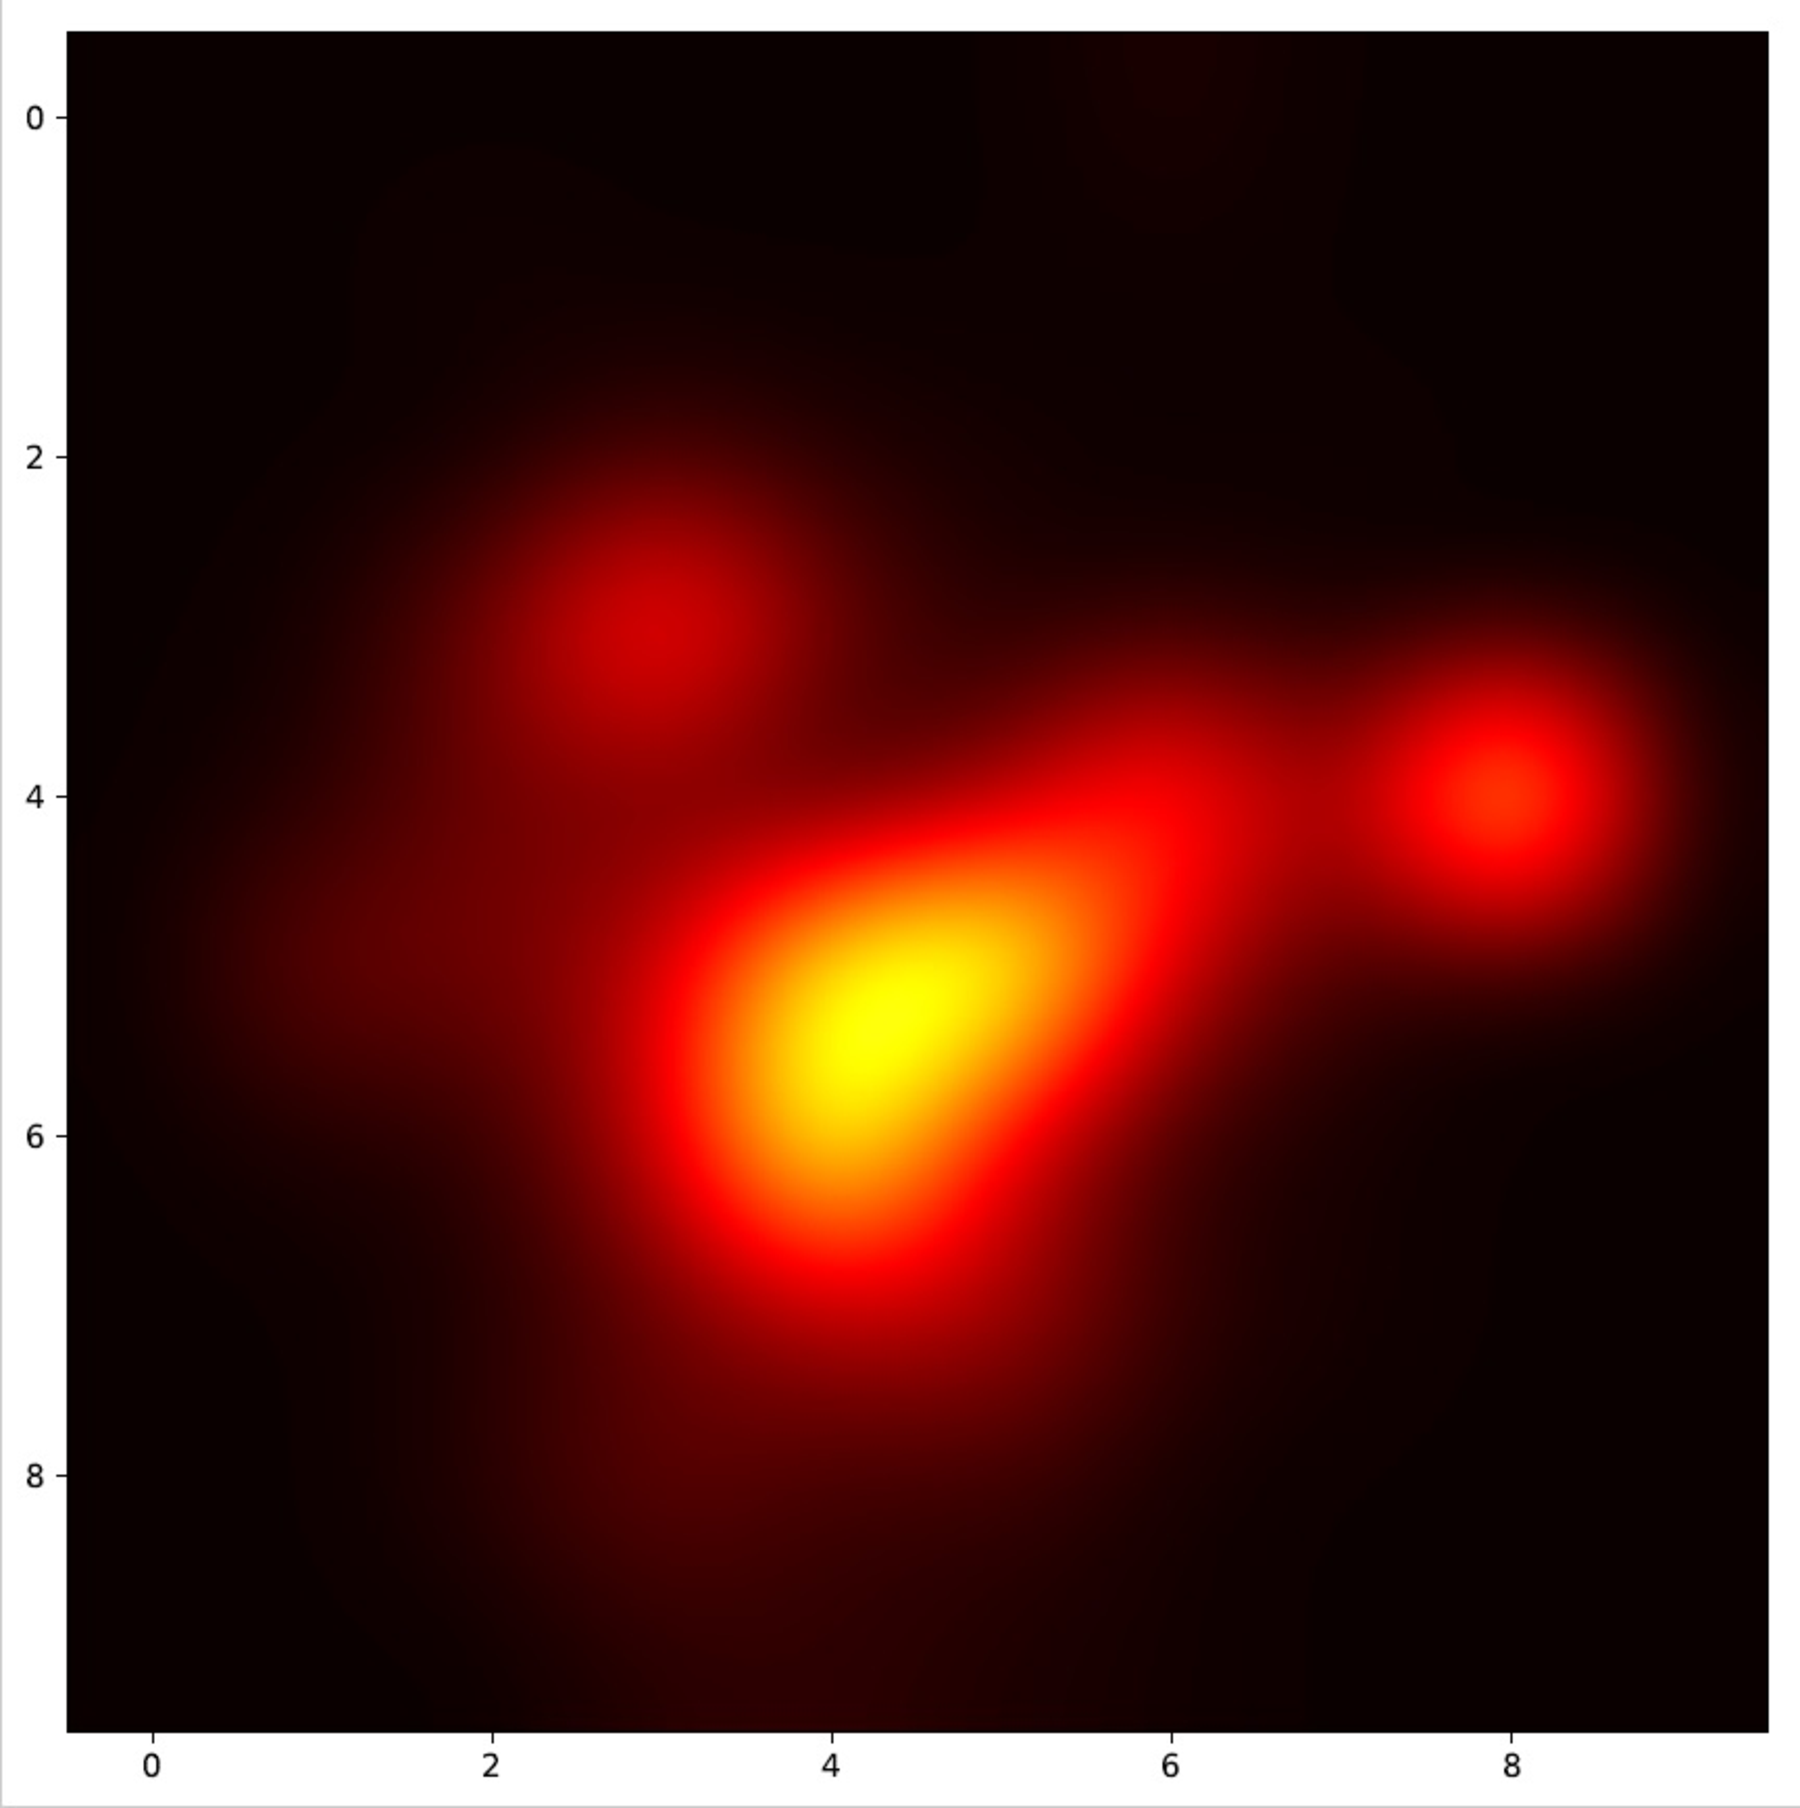
\includegraphics[width=\textwidth]{./figs/6mil_HSphere.pdf}
			\end{subfigure}
			\begin{subfigure}[b]{0.23\textwidth}
				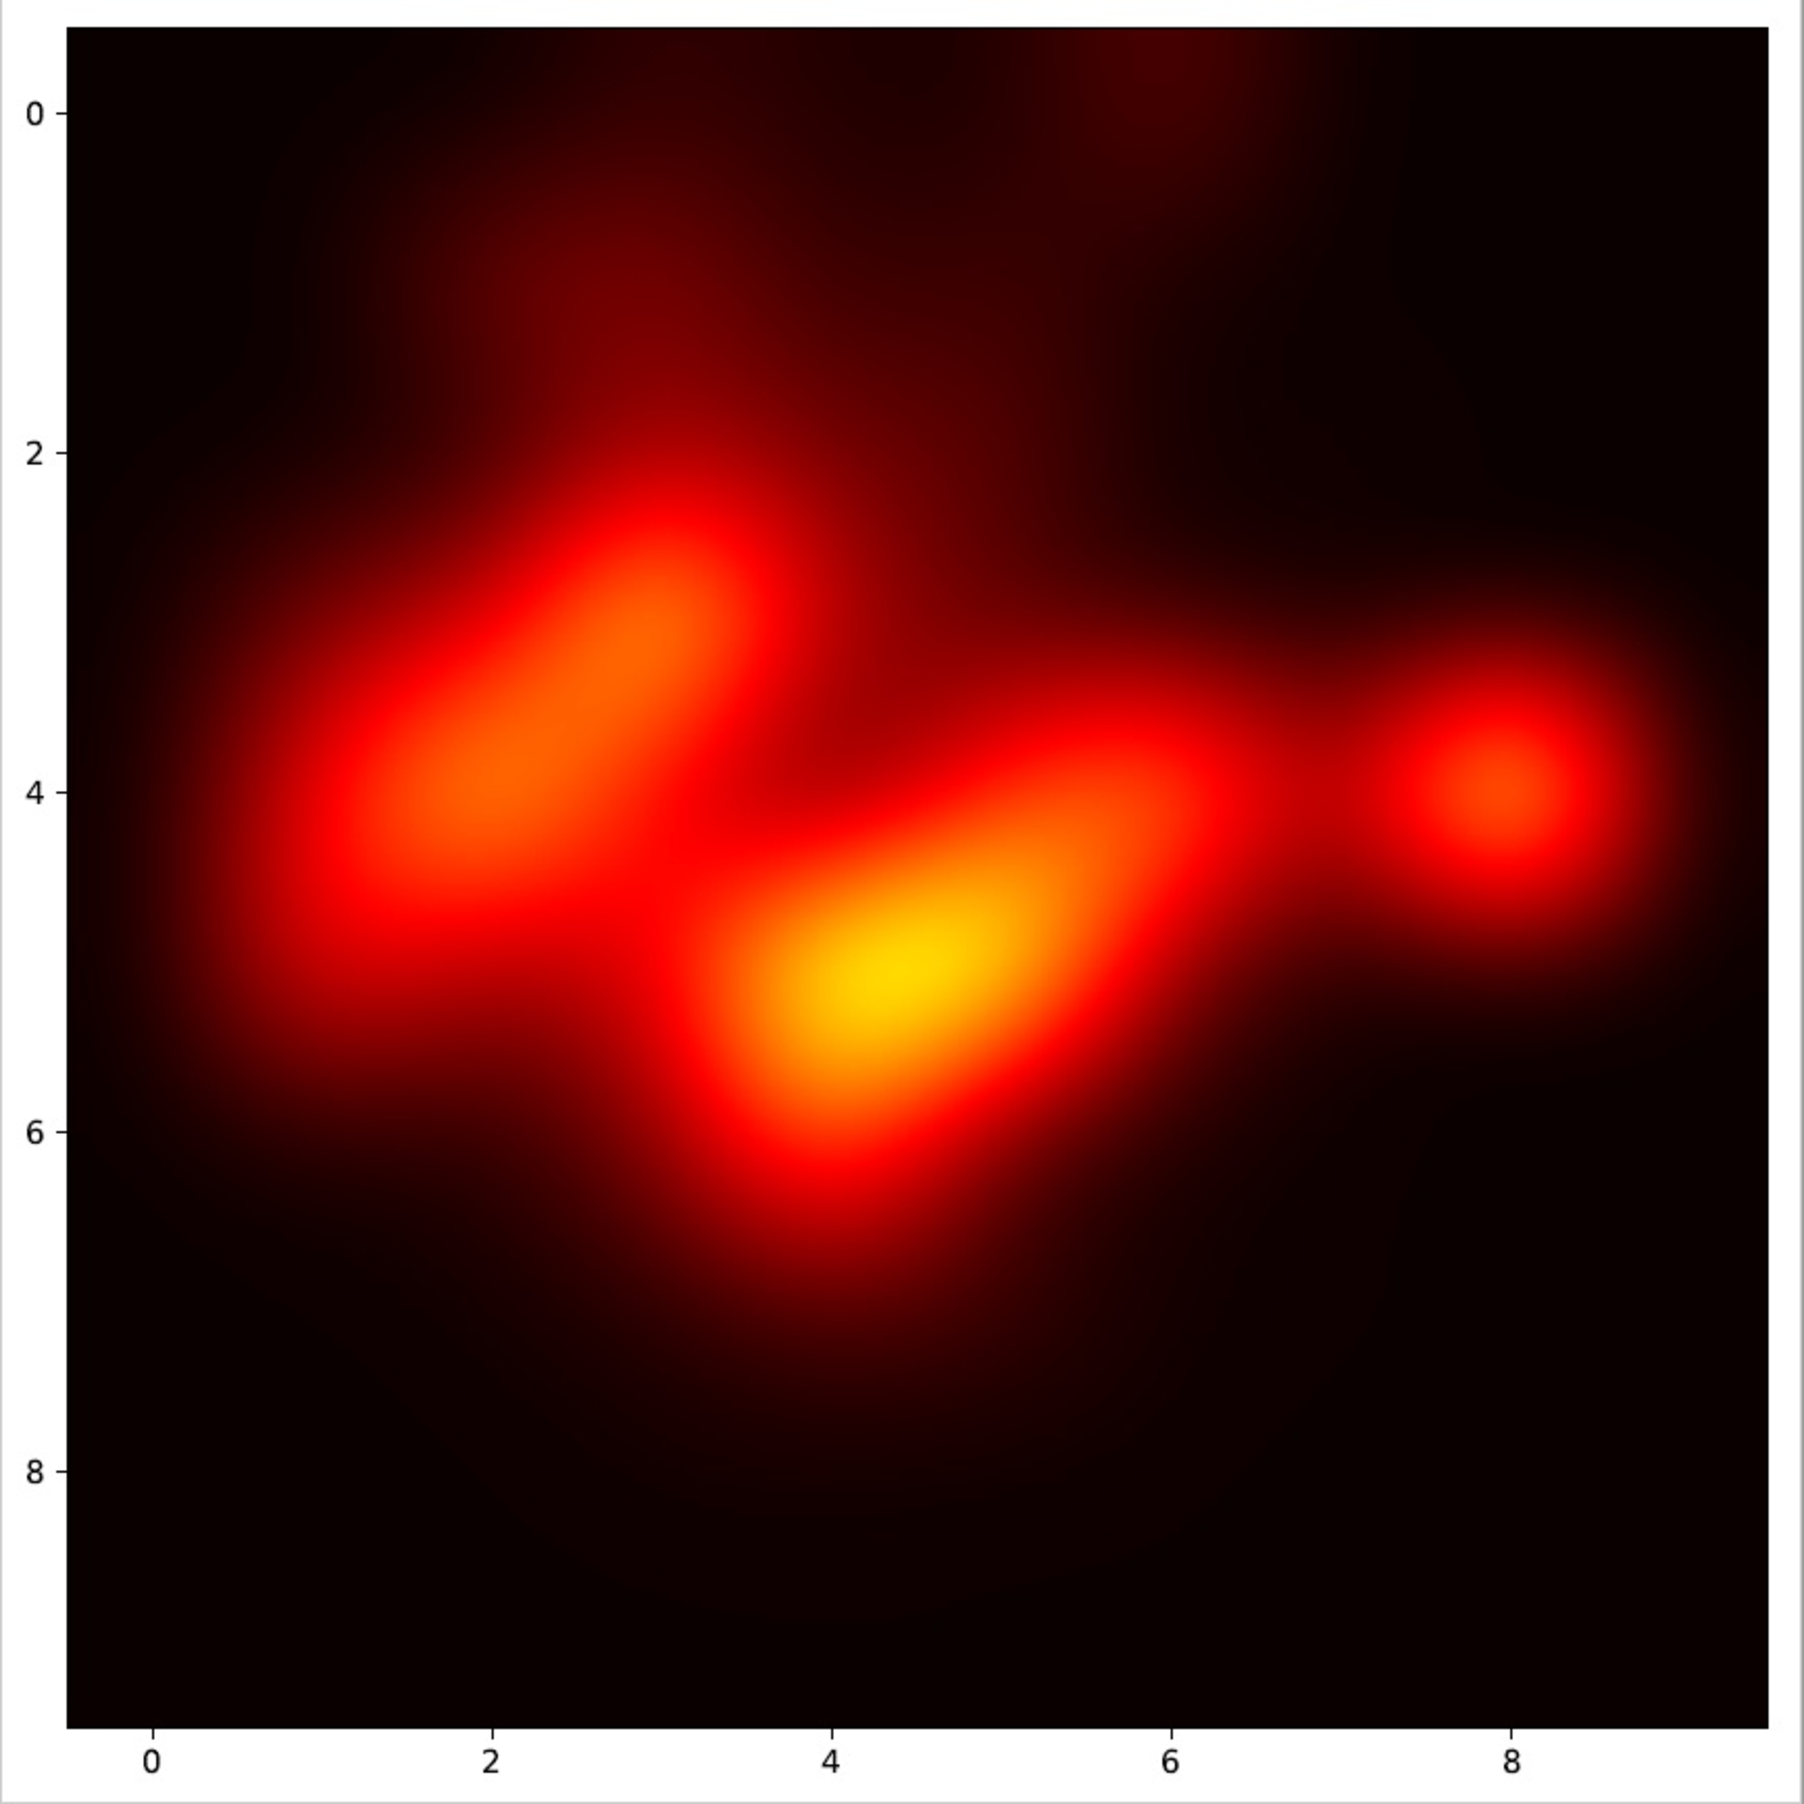
\includegraphics[width=\textwidth]{./figs/6mil_HCube.pdf}
			\end{subfigure}\\
		\end{subfigure}
		\vspace{-0.9em}
		\begin{subfigure}[b]{\textwidth}
			\begin{subfigure}[b]{0.04\textwidth}
				
\includegraphics[width=\textwidth]{./figs/10mil_label.jpg}
			\end{subfigure}
			\begin{subfigure}[b]{0.23\textwidth}
				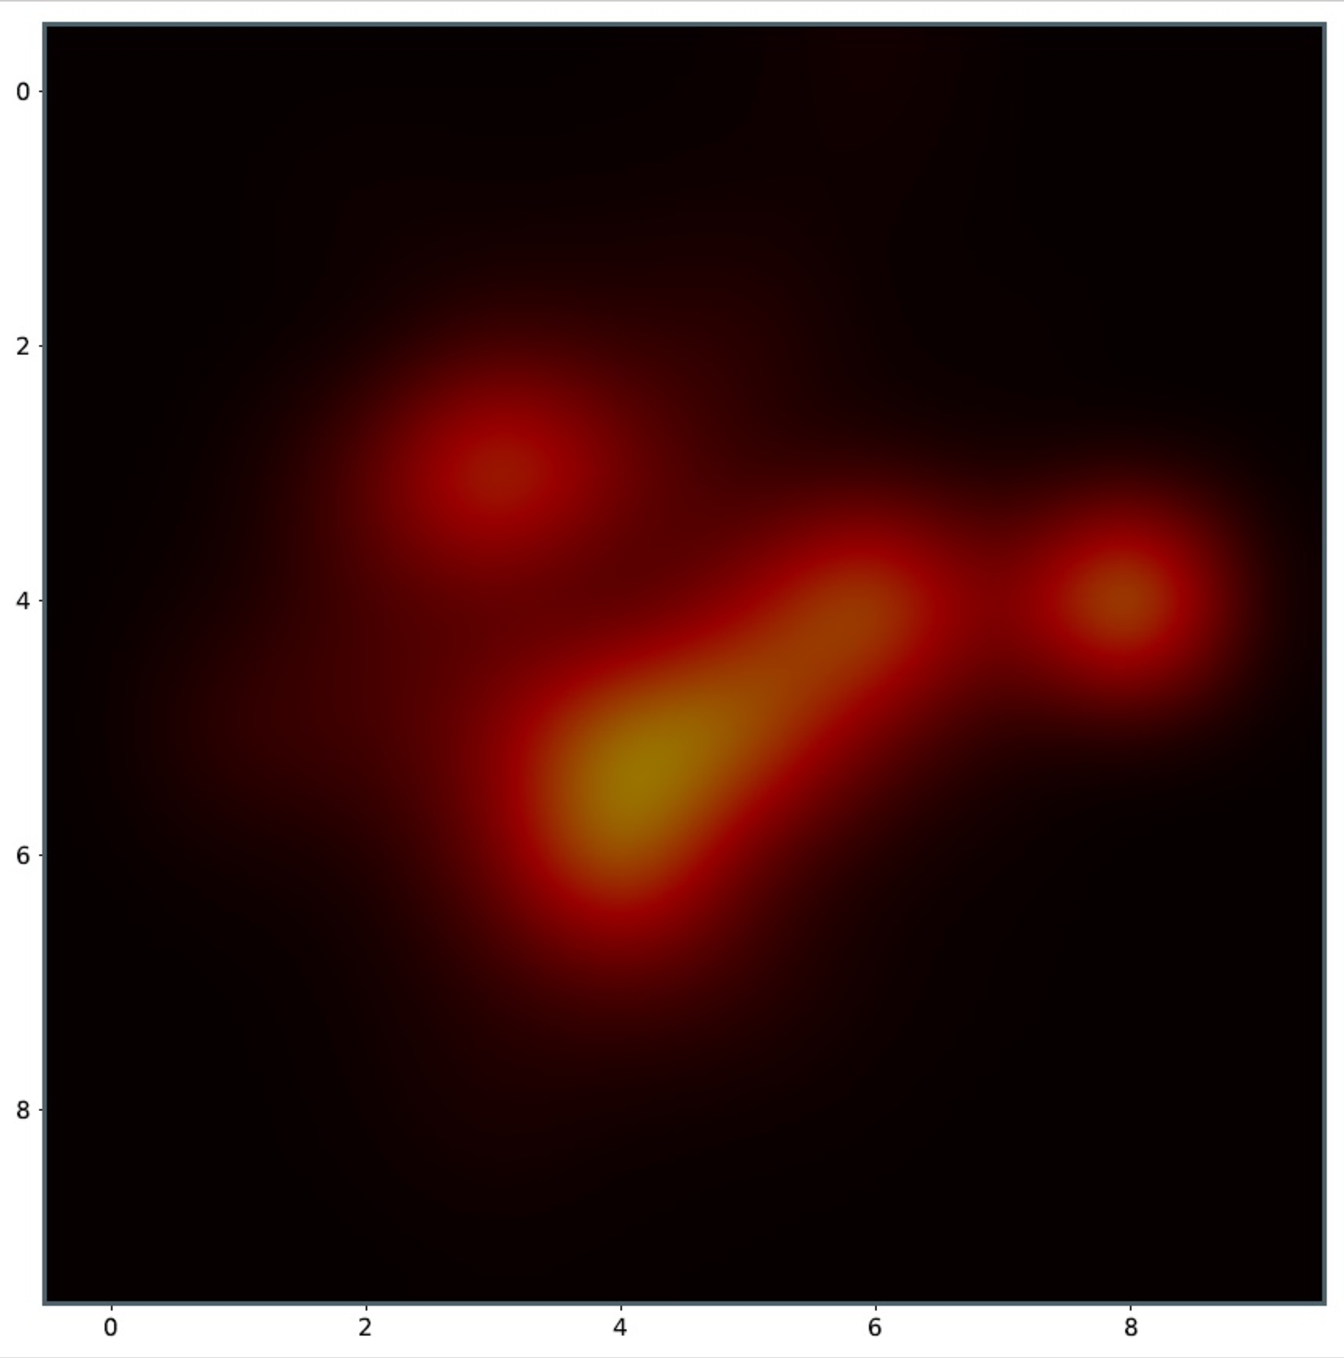
\includegraphics[width=\textwidth]{./figs/10mil_Sphere.pdf}
			\end{subfigure}
			\begin{subfigure}[b]{0.23\textwidth}
				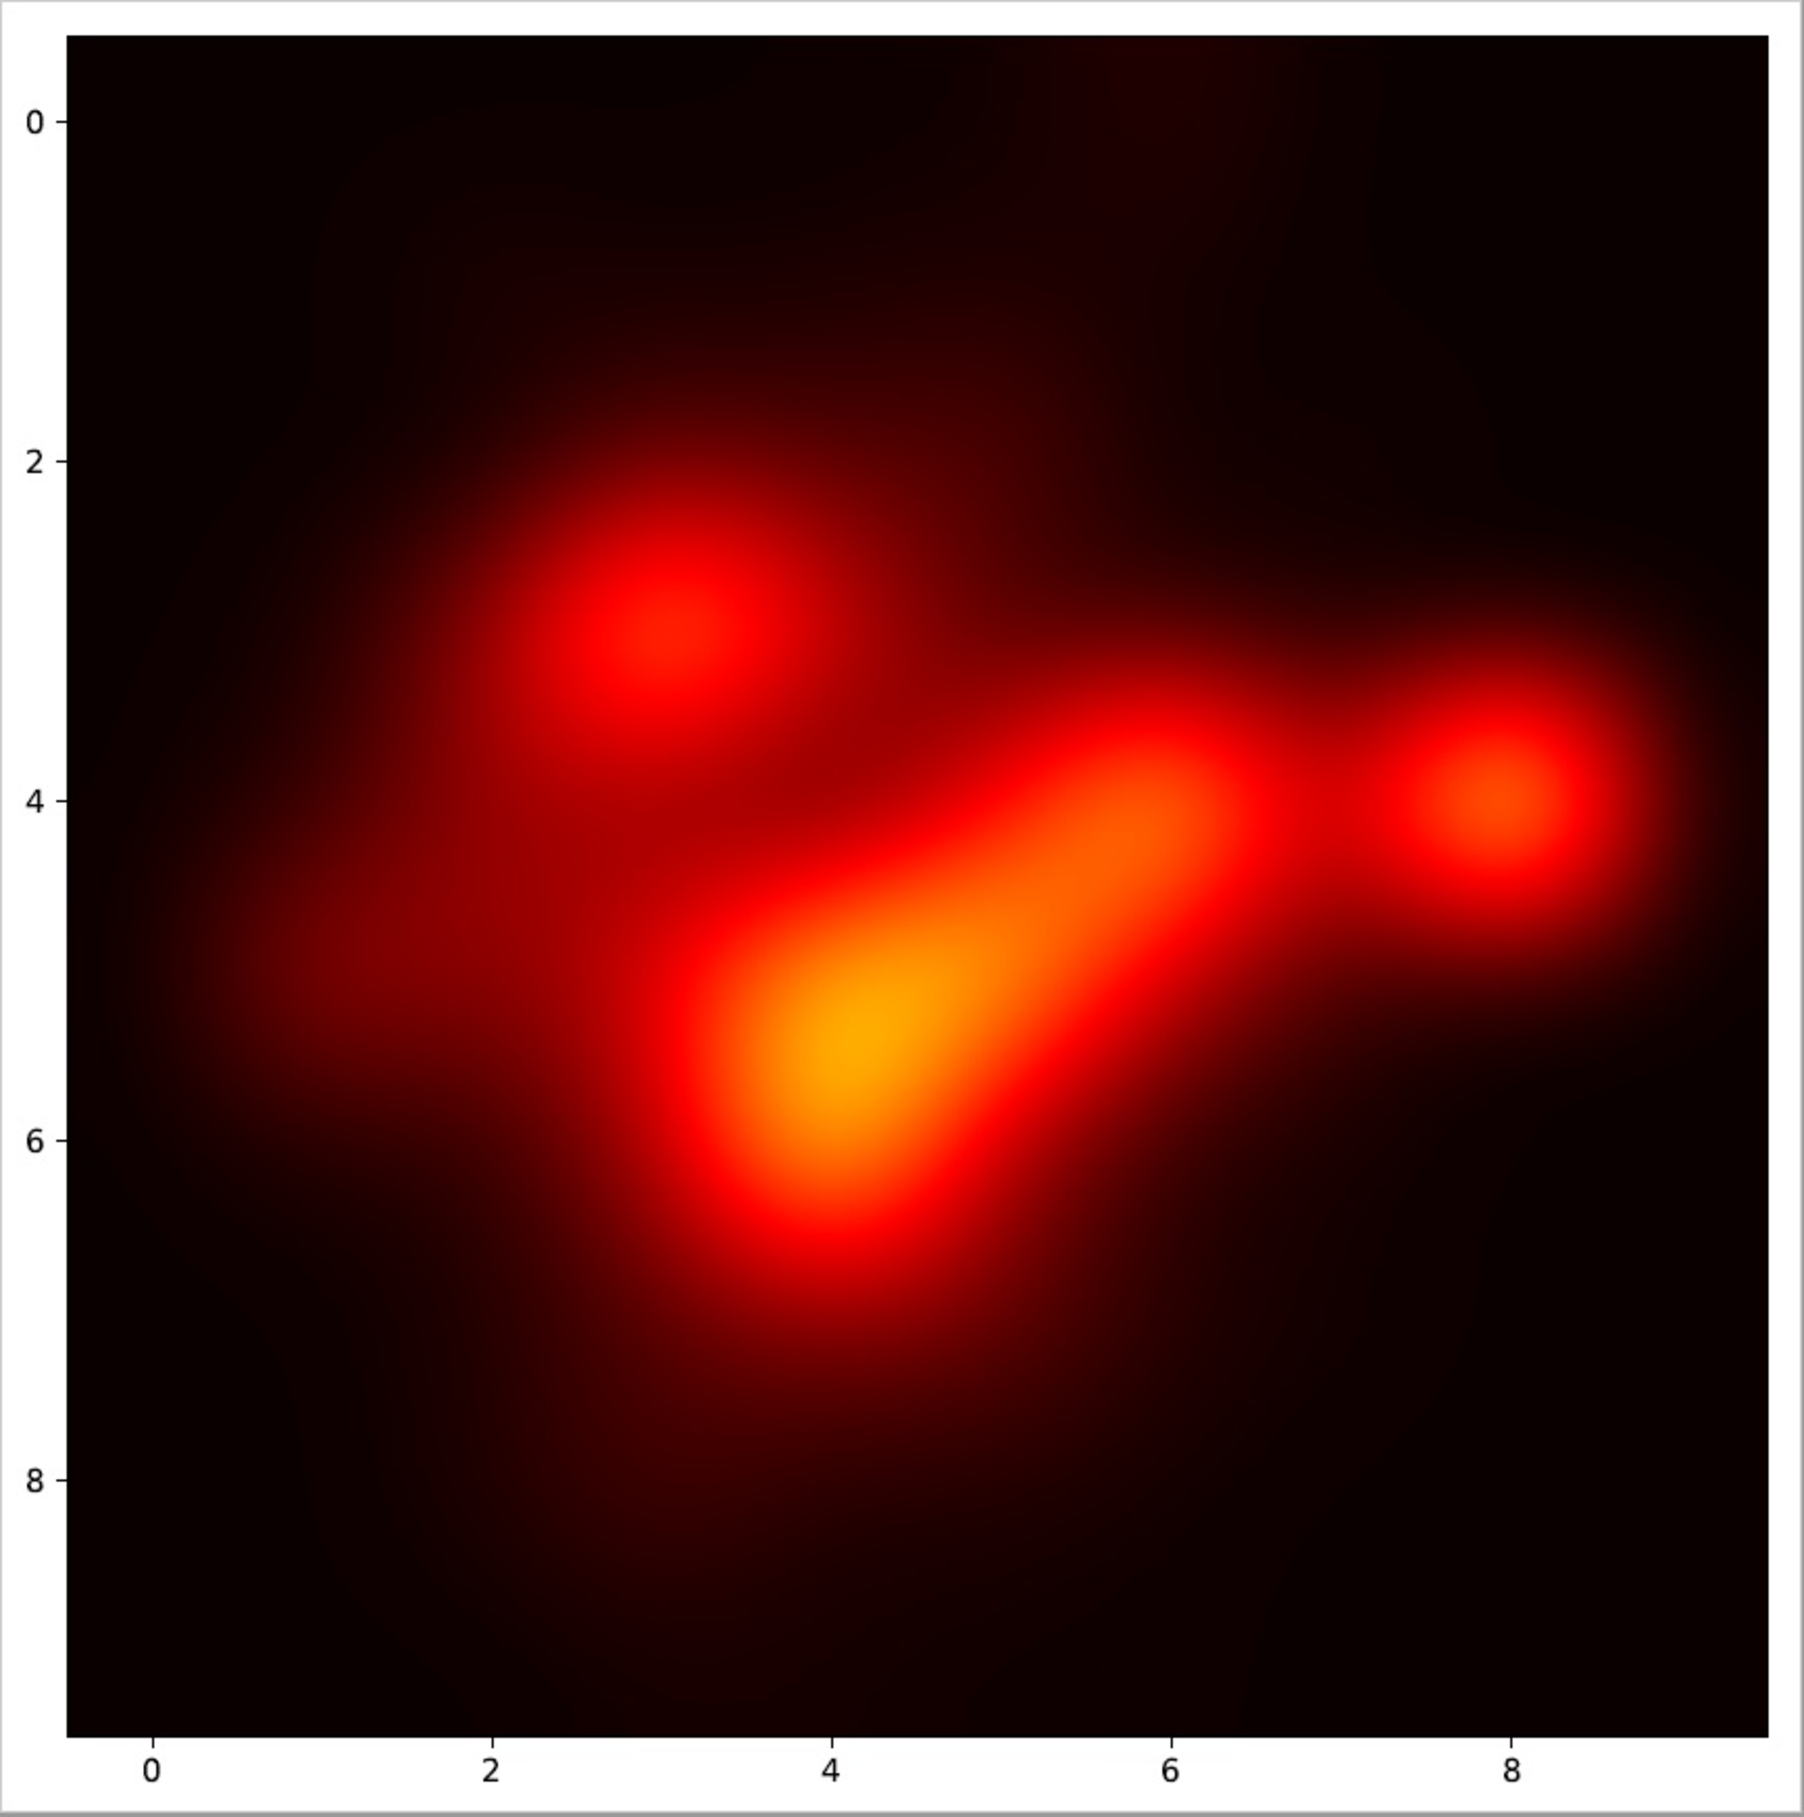
\includegraphics[width=\textwidth]{./figs/10mil_Cube.pdf}
			\end{subfigure}
			\begin{subfigure}[b]{0.23\textwidth}
				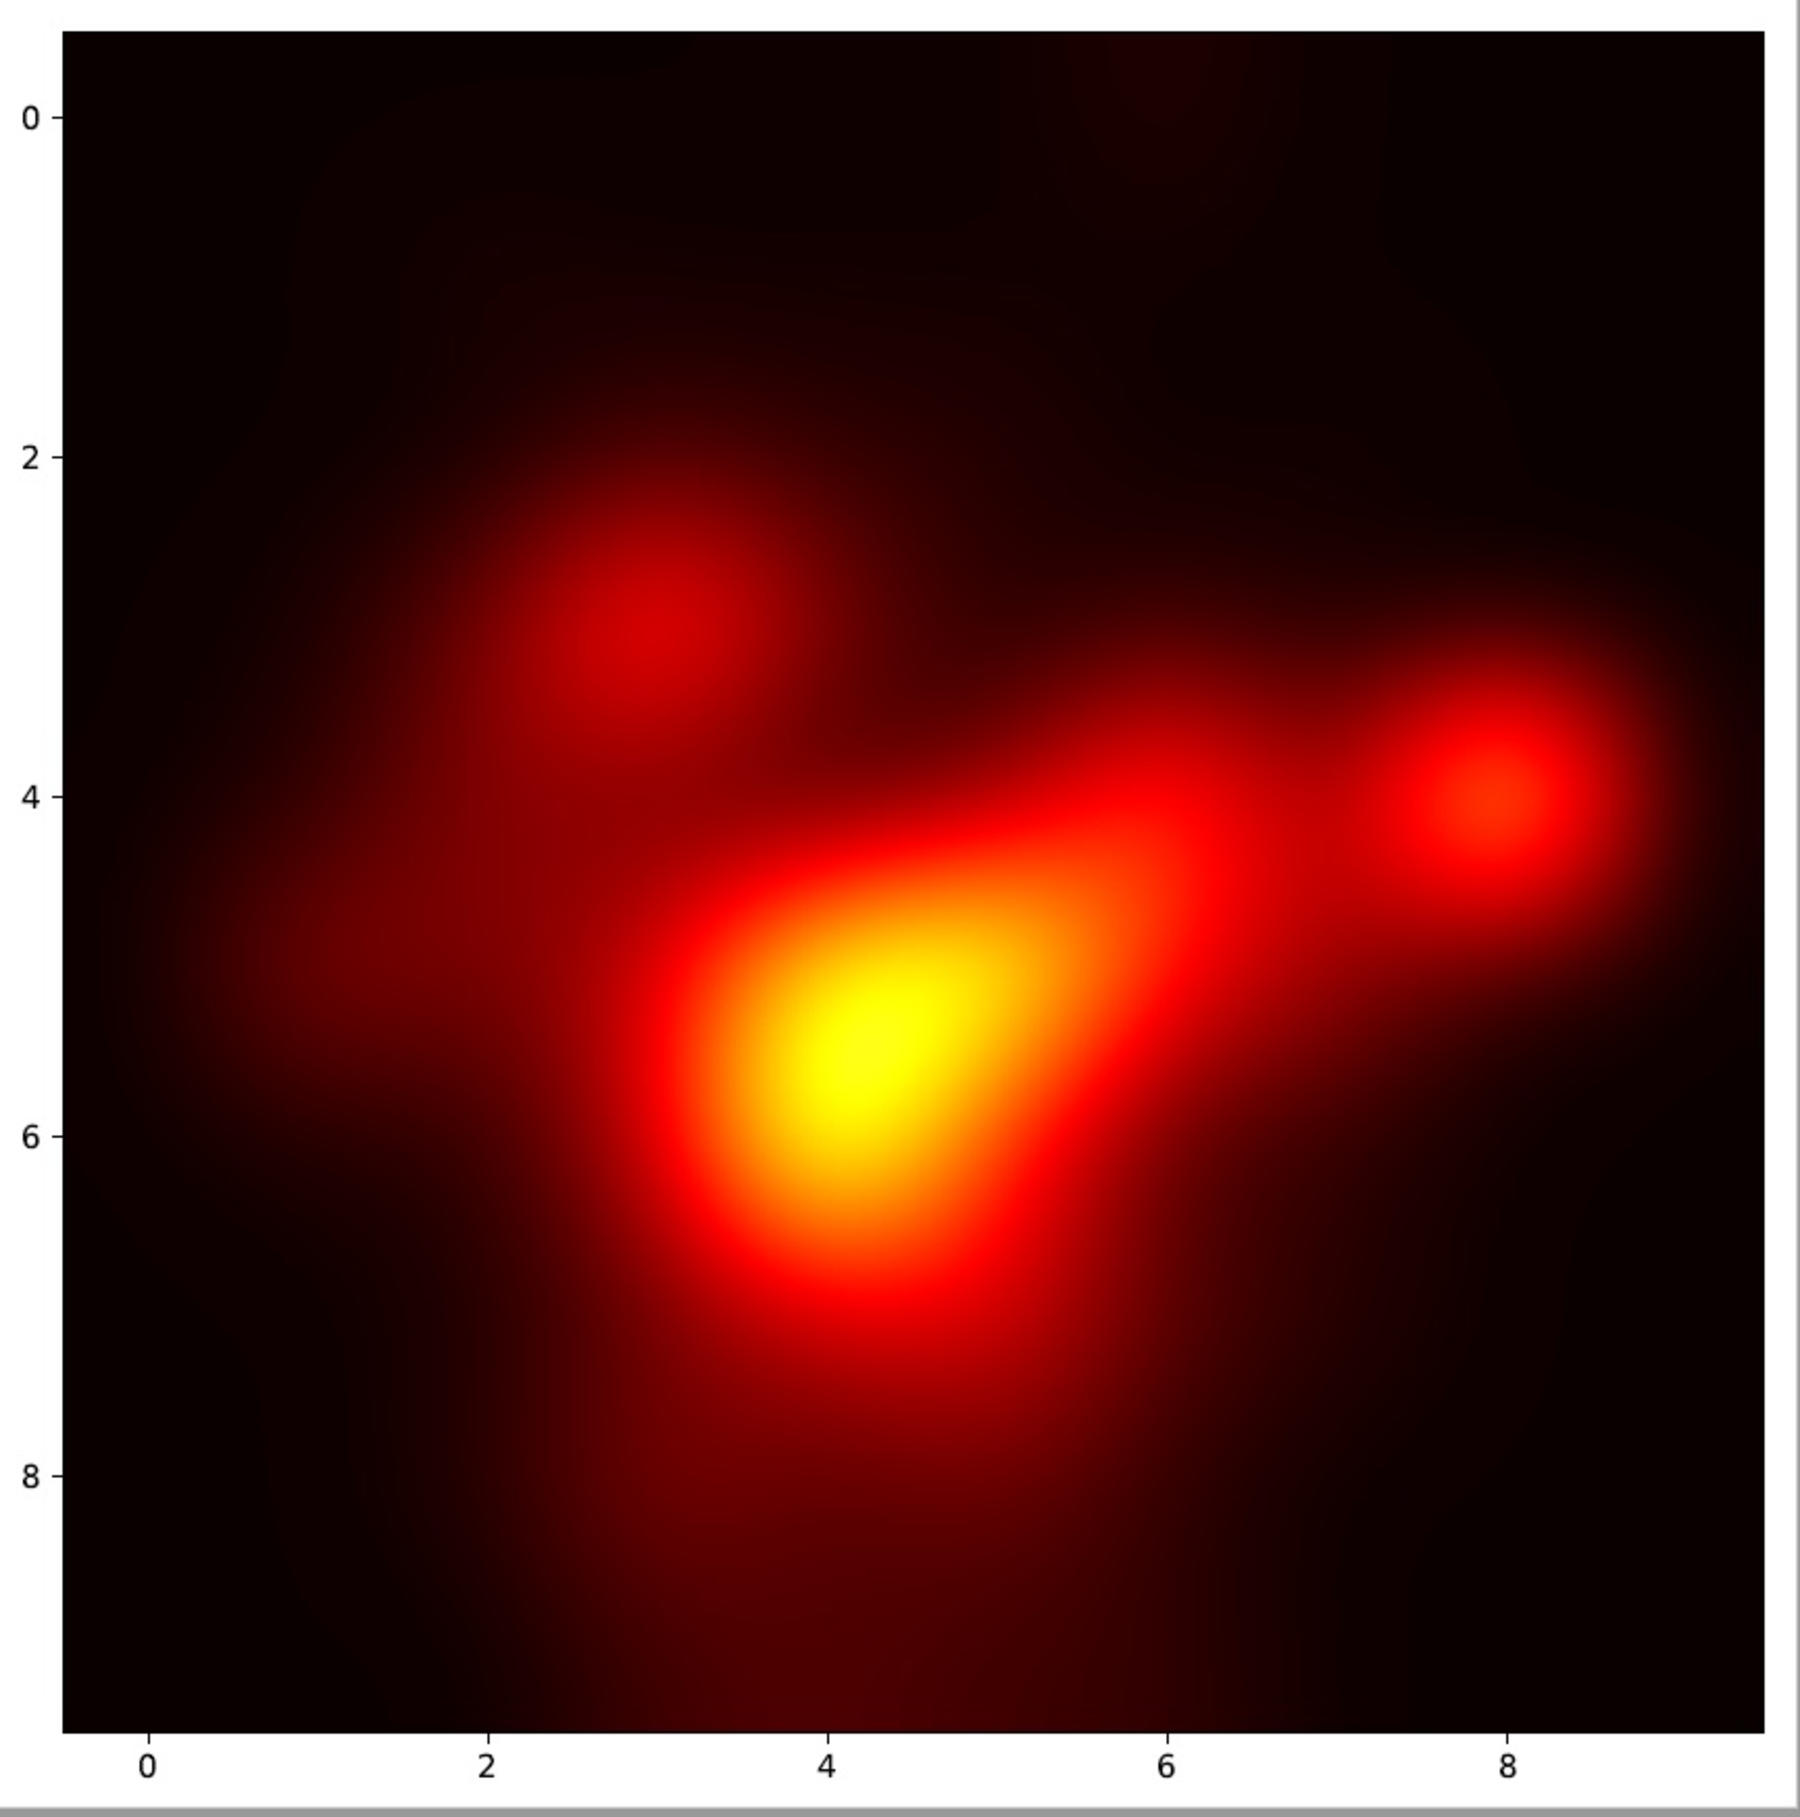
\includegraphics[width=\textwidth]{./figs/10mil_HSphere.pdf}
			\end{subfigure}
			\begin{subfigure}[b]{0.23\textwidth}
				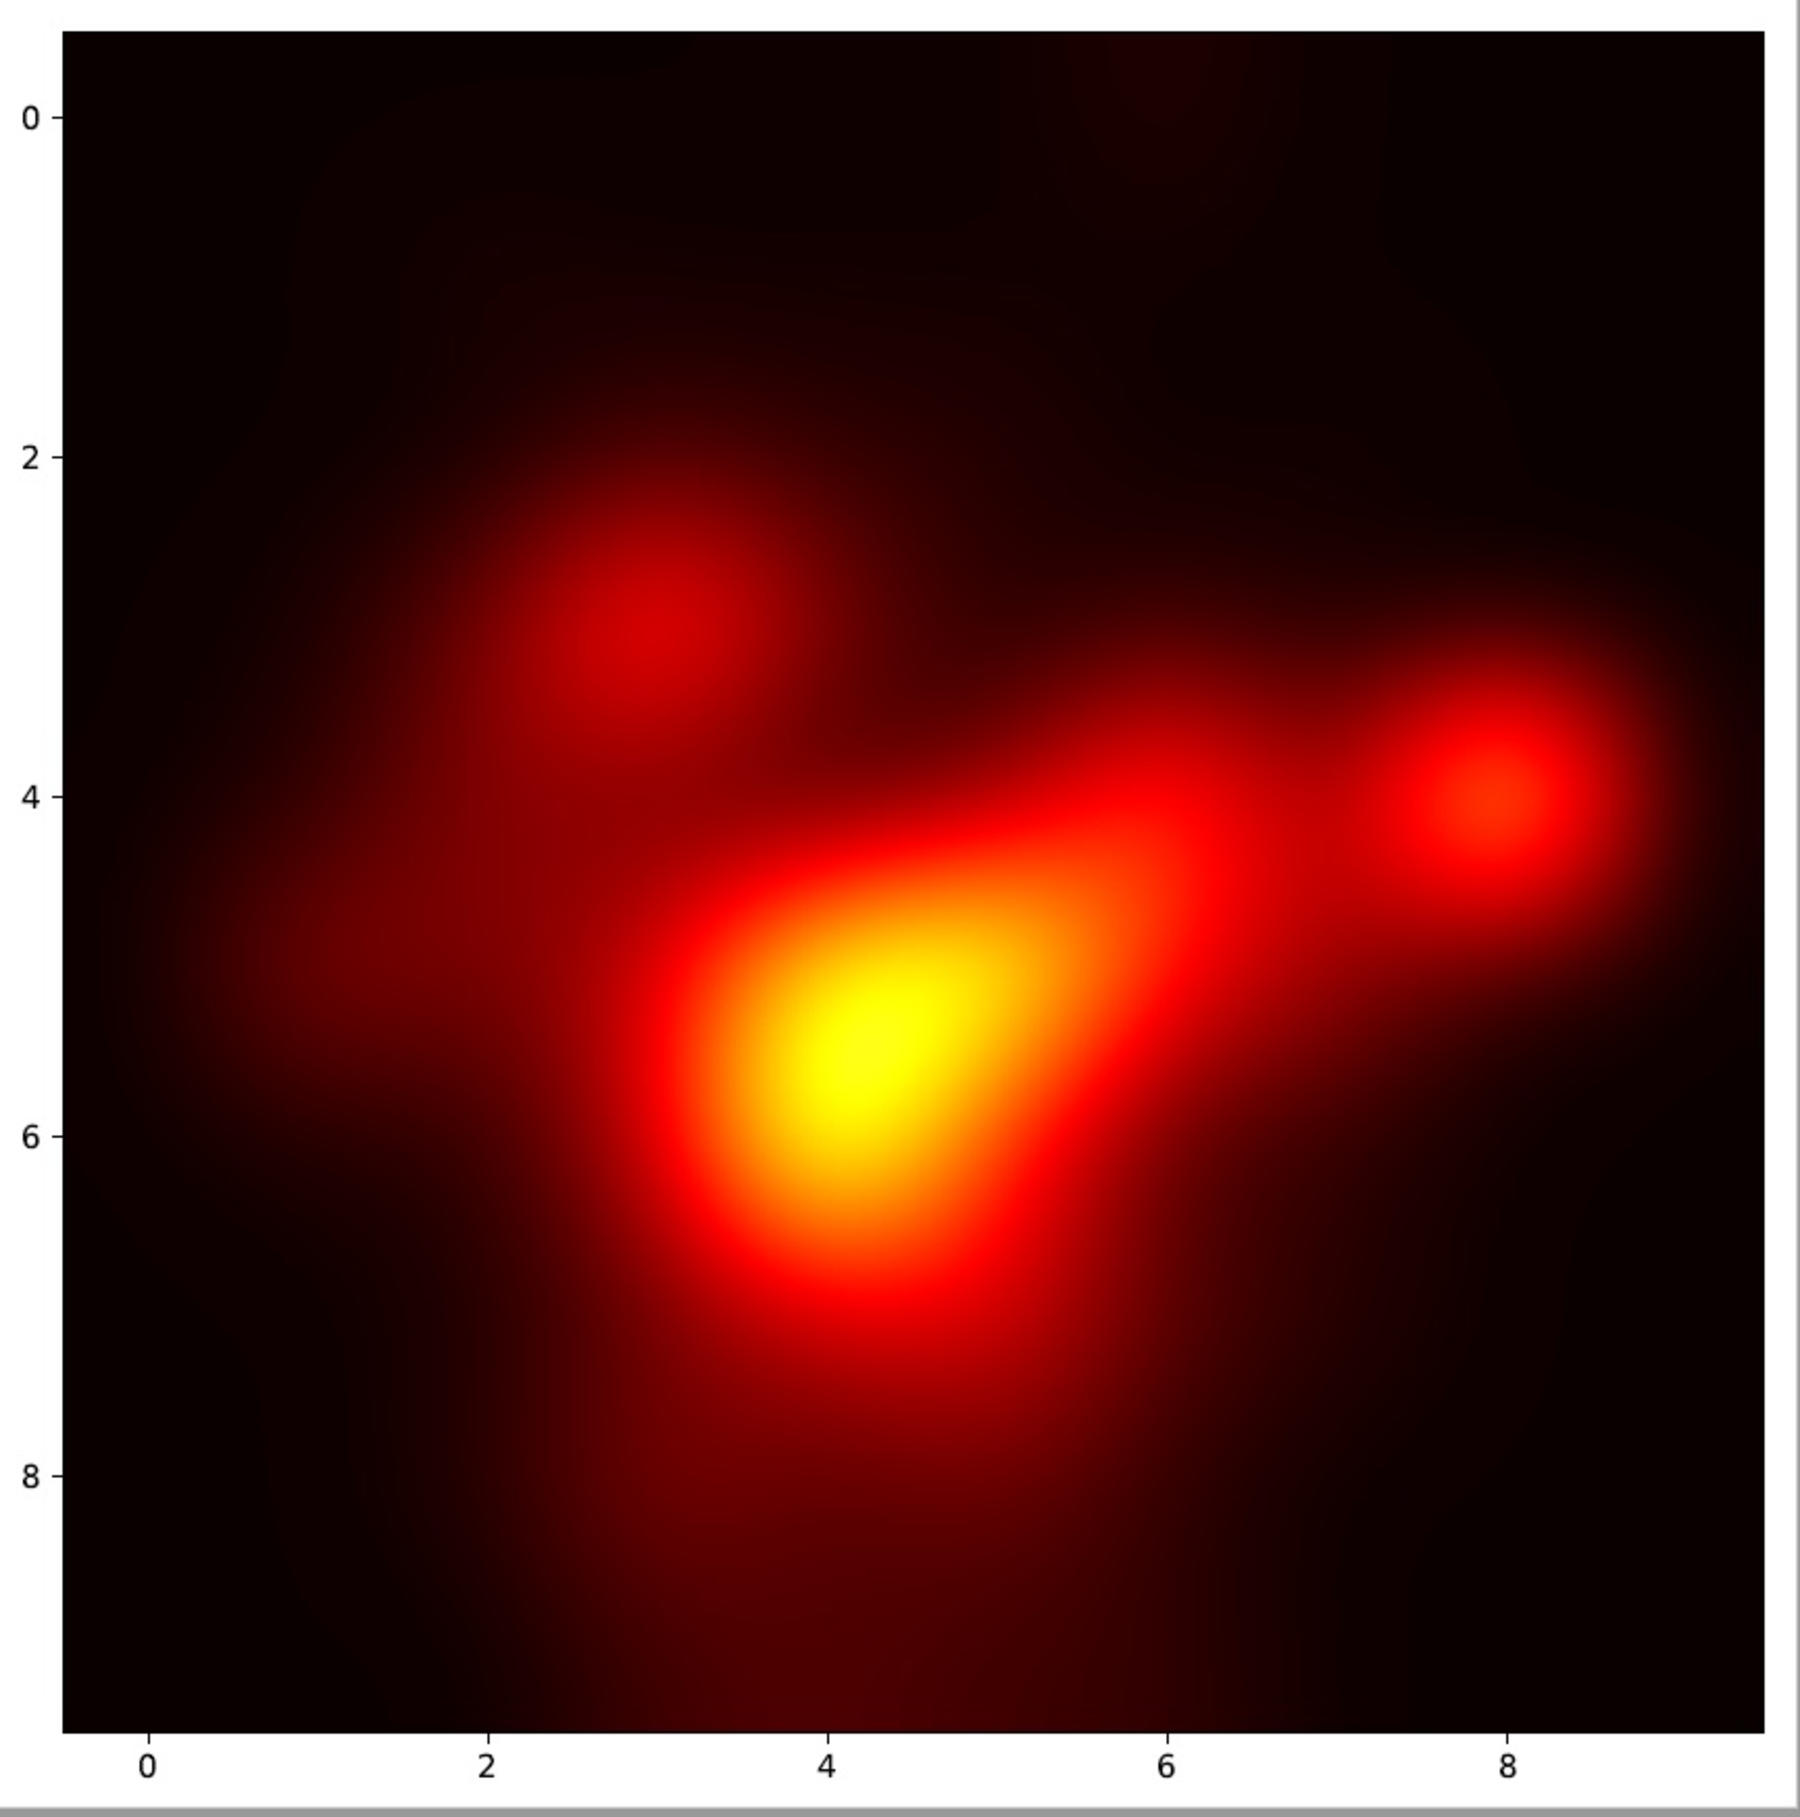
\includegraphics[width=\textwidth]{./figs/10mil_HCube.pdf}
			\end{subfigure}
		\end{subfigure}
		\vspace*{0.9em}
	\end{subfigure}
\caption{3D-printed Sphere, Cube, Half-Cylinder and Cuboid (view from above) and relative tactile images computed (averaged sensor readings over three trials).}
\label{parts}
\end{figure} 
\begin{figure}[]
	\centering
	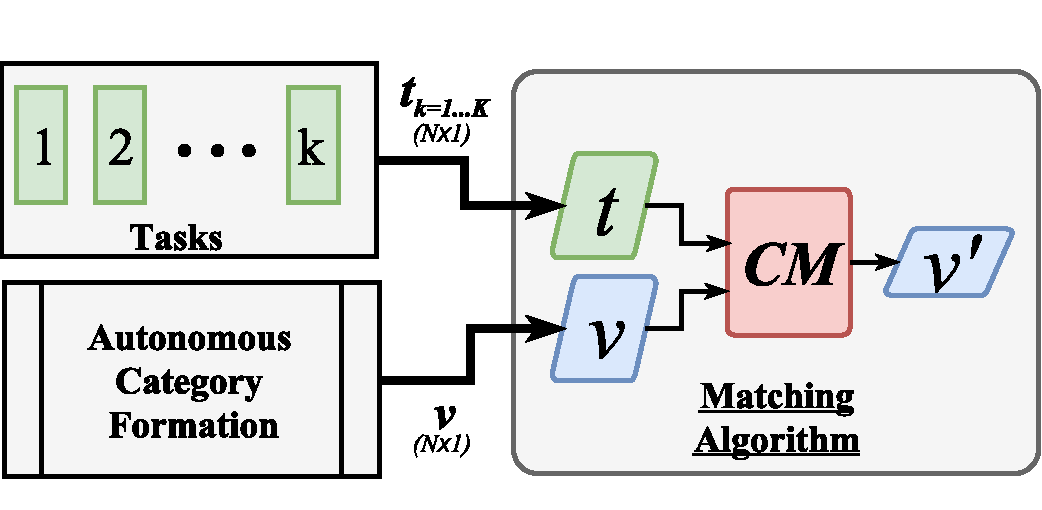
\includegraphics[width=.45\textwidth]{./figs/cluster_matching.pdf}
	\caption{Process pipeline for the Cluster Matching Algorithm.}
	\label{cluster_matching}
	\vspace{15pt}
\end{figure}
The unsupervised part of the process (PCA \& KMC) clusters the objects automatically based on the two dimensions of highest variance in the data. We define the cluster matching process $\mathbf{CM}$ as:
\begin{equation}
\vec{v}^{\ \prime} = \mathbf{CM}(\vec{v},\ \vec{t}_k)
\end{equation}
Given a task $\vec{t}_k$ and a cluster guess vector $\vec{v}$ then, $\vec{v}\ '$ is a new vector such that 
\begin{flalign*}
&\forall i \in \{1,2, ... , N\}.\\
&\  (\vec{v}_i =1 \implies \vec{v}_i^{\ \prime}=0) \land  (\vec{v}_i =0 \implies \vec{v}_i^{\ \prime}=1)\\
&\iff\ ||\vec{v}-\vec{t}_k||>||\vec{v}_i^{\ \prime}-\vec{t}_k||
\end{flalign*} 
i.e. we associate a cluster guess to a target cluster maximizing accuracy on a particular task (Fig. \ref{cluster_matching}). A vector $\vec{v}=[0\ 0\ 0\ 1]$ for a task $\vec{t}_k=[1\ 1\ 1\ 0]$, for example, would be re-associated as $\vec{v}^{\ \prime}=[1\ 1\ 1\ 0]$. We utilize this to benchmark the performance of the algorithm in the various tasks (the object's inclusion in a cluster does not change after matching).  


\section{EXPERIMENTAL RESULTS}
\label{exp}
\begin{figure}[]
	\centering
	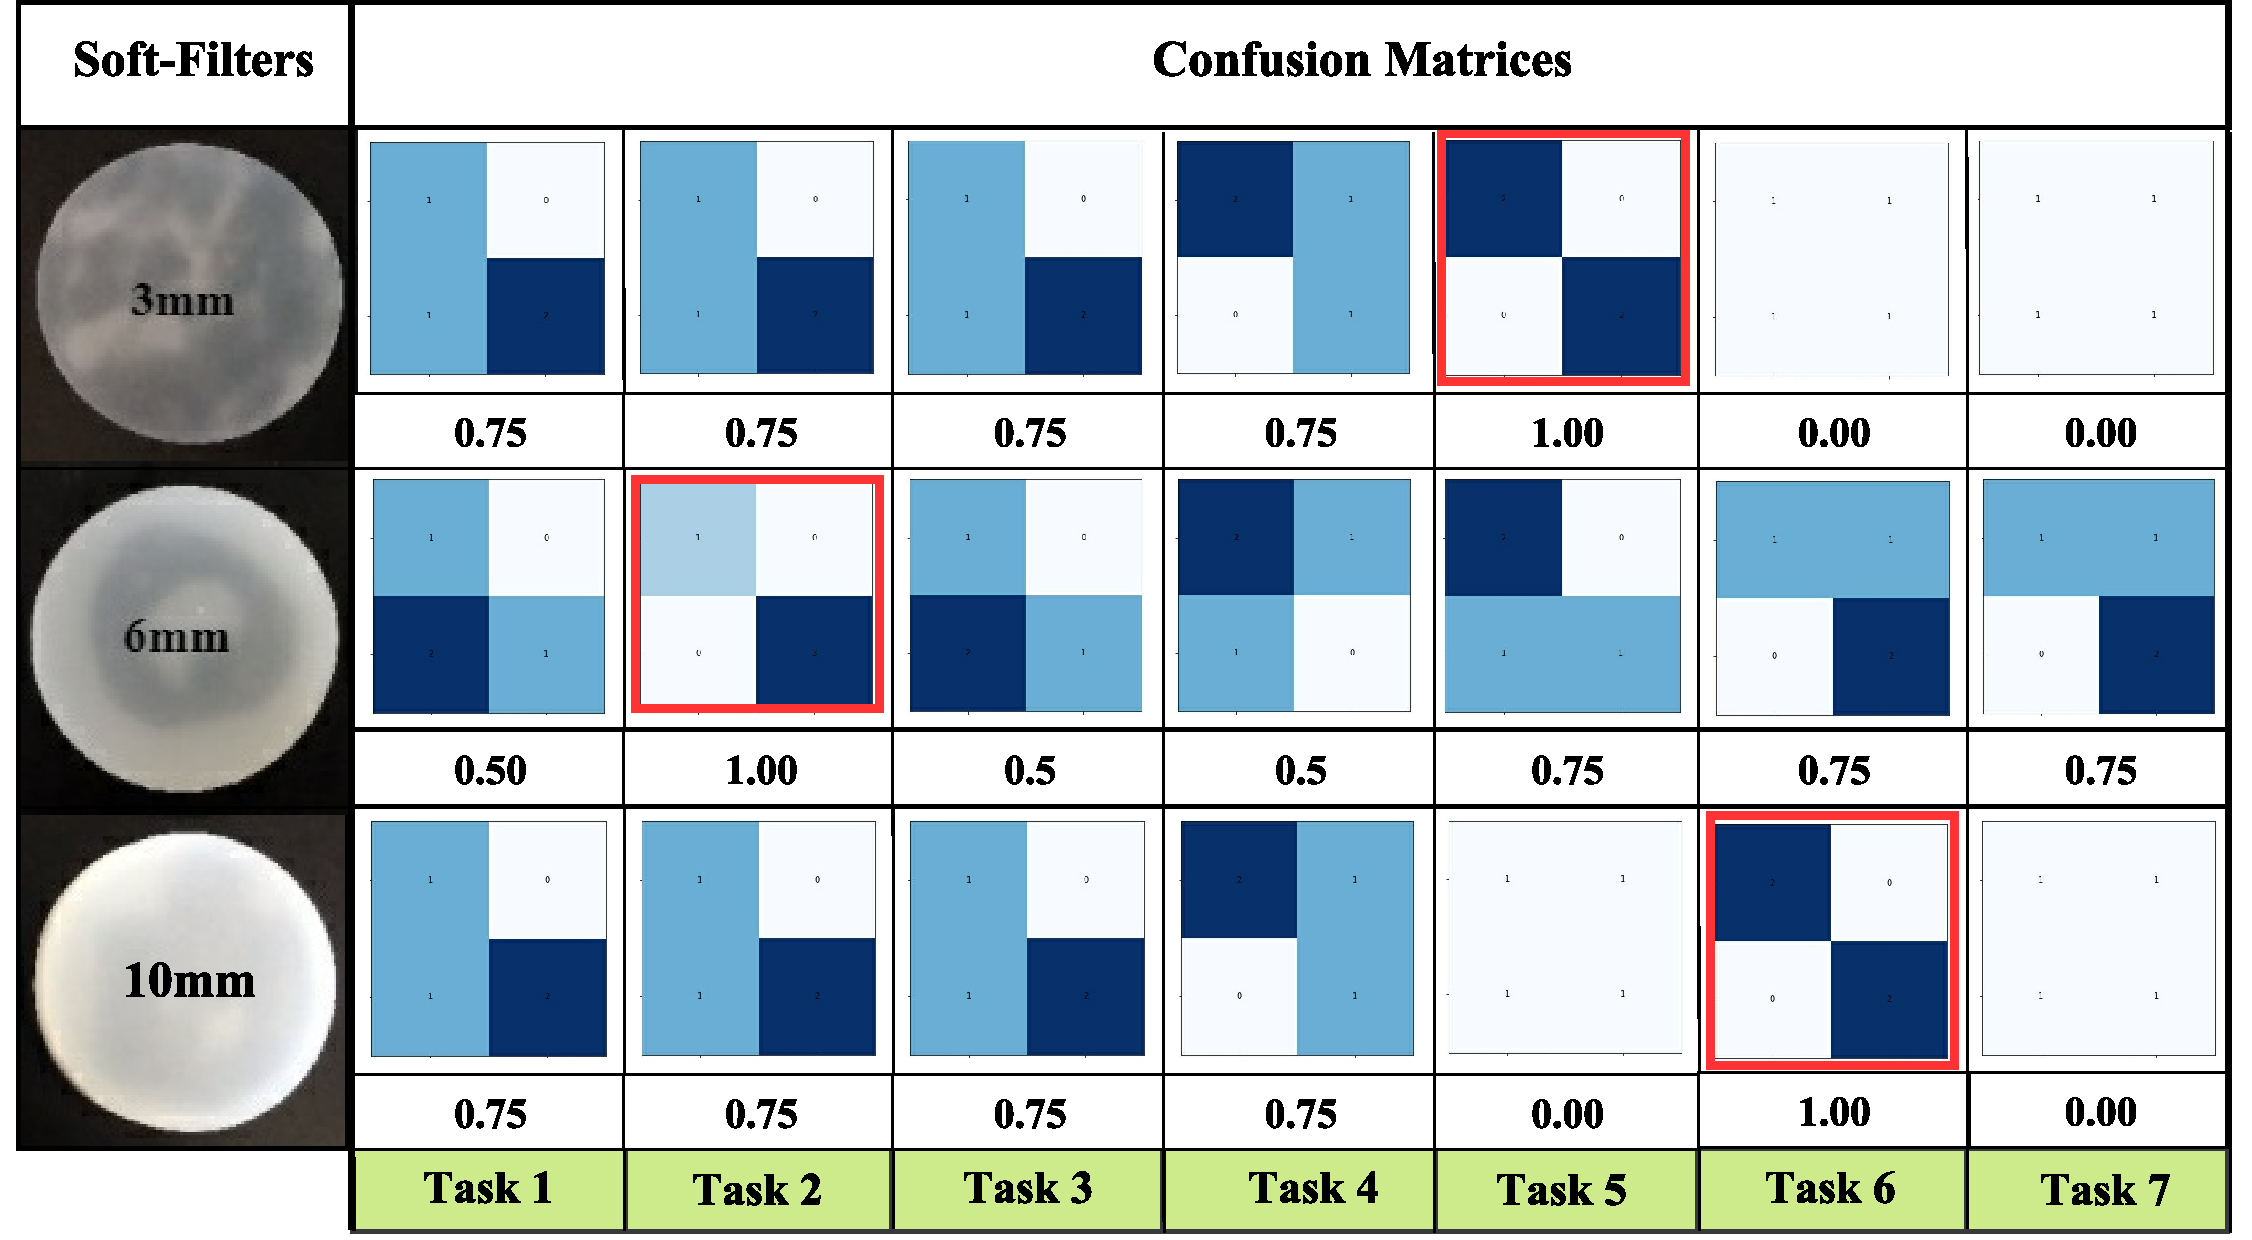
\includegraphics[width=0.45\textwidth]{./figs/conf_results.pdf}
	\caption{Confusion matrices and accuracy values for 7 different tasks corresponding to the clustering results obtained with three soft filters of $3mm$, $6mm$ and $10mm$ respectively. The diagonal in each matrix retains the counts for the correct cluster guesses. Each soft filter is optimized for a specific task, highlighted in red.}
	\label{conf_results}
	\vspace{10pt}
\end{figure}
\subsection{Task Optimization}
After the experiments, we observe the accuracy of the clustering with respect to the 7 predefined tasks. Fig. \ref{conf_results} illustrates the resulting confusion matrices. For each $(2\times 2)$ confusion matrix $\mathbf{C}$, the darkness in square $C_{ij}$ is proportional to the number of times an object class $i$ was matched to a object guess $j$. The main diagonal then, contains the counts for the correct guesses, while anything outside of it is a mismatch.
As clear from the figure each of the soft filters alters 
\begin{figure}[H]
	\centering
	\begin{subfigure}[b]{0.4\textwidth}
		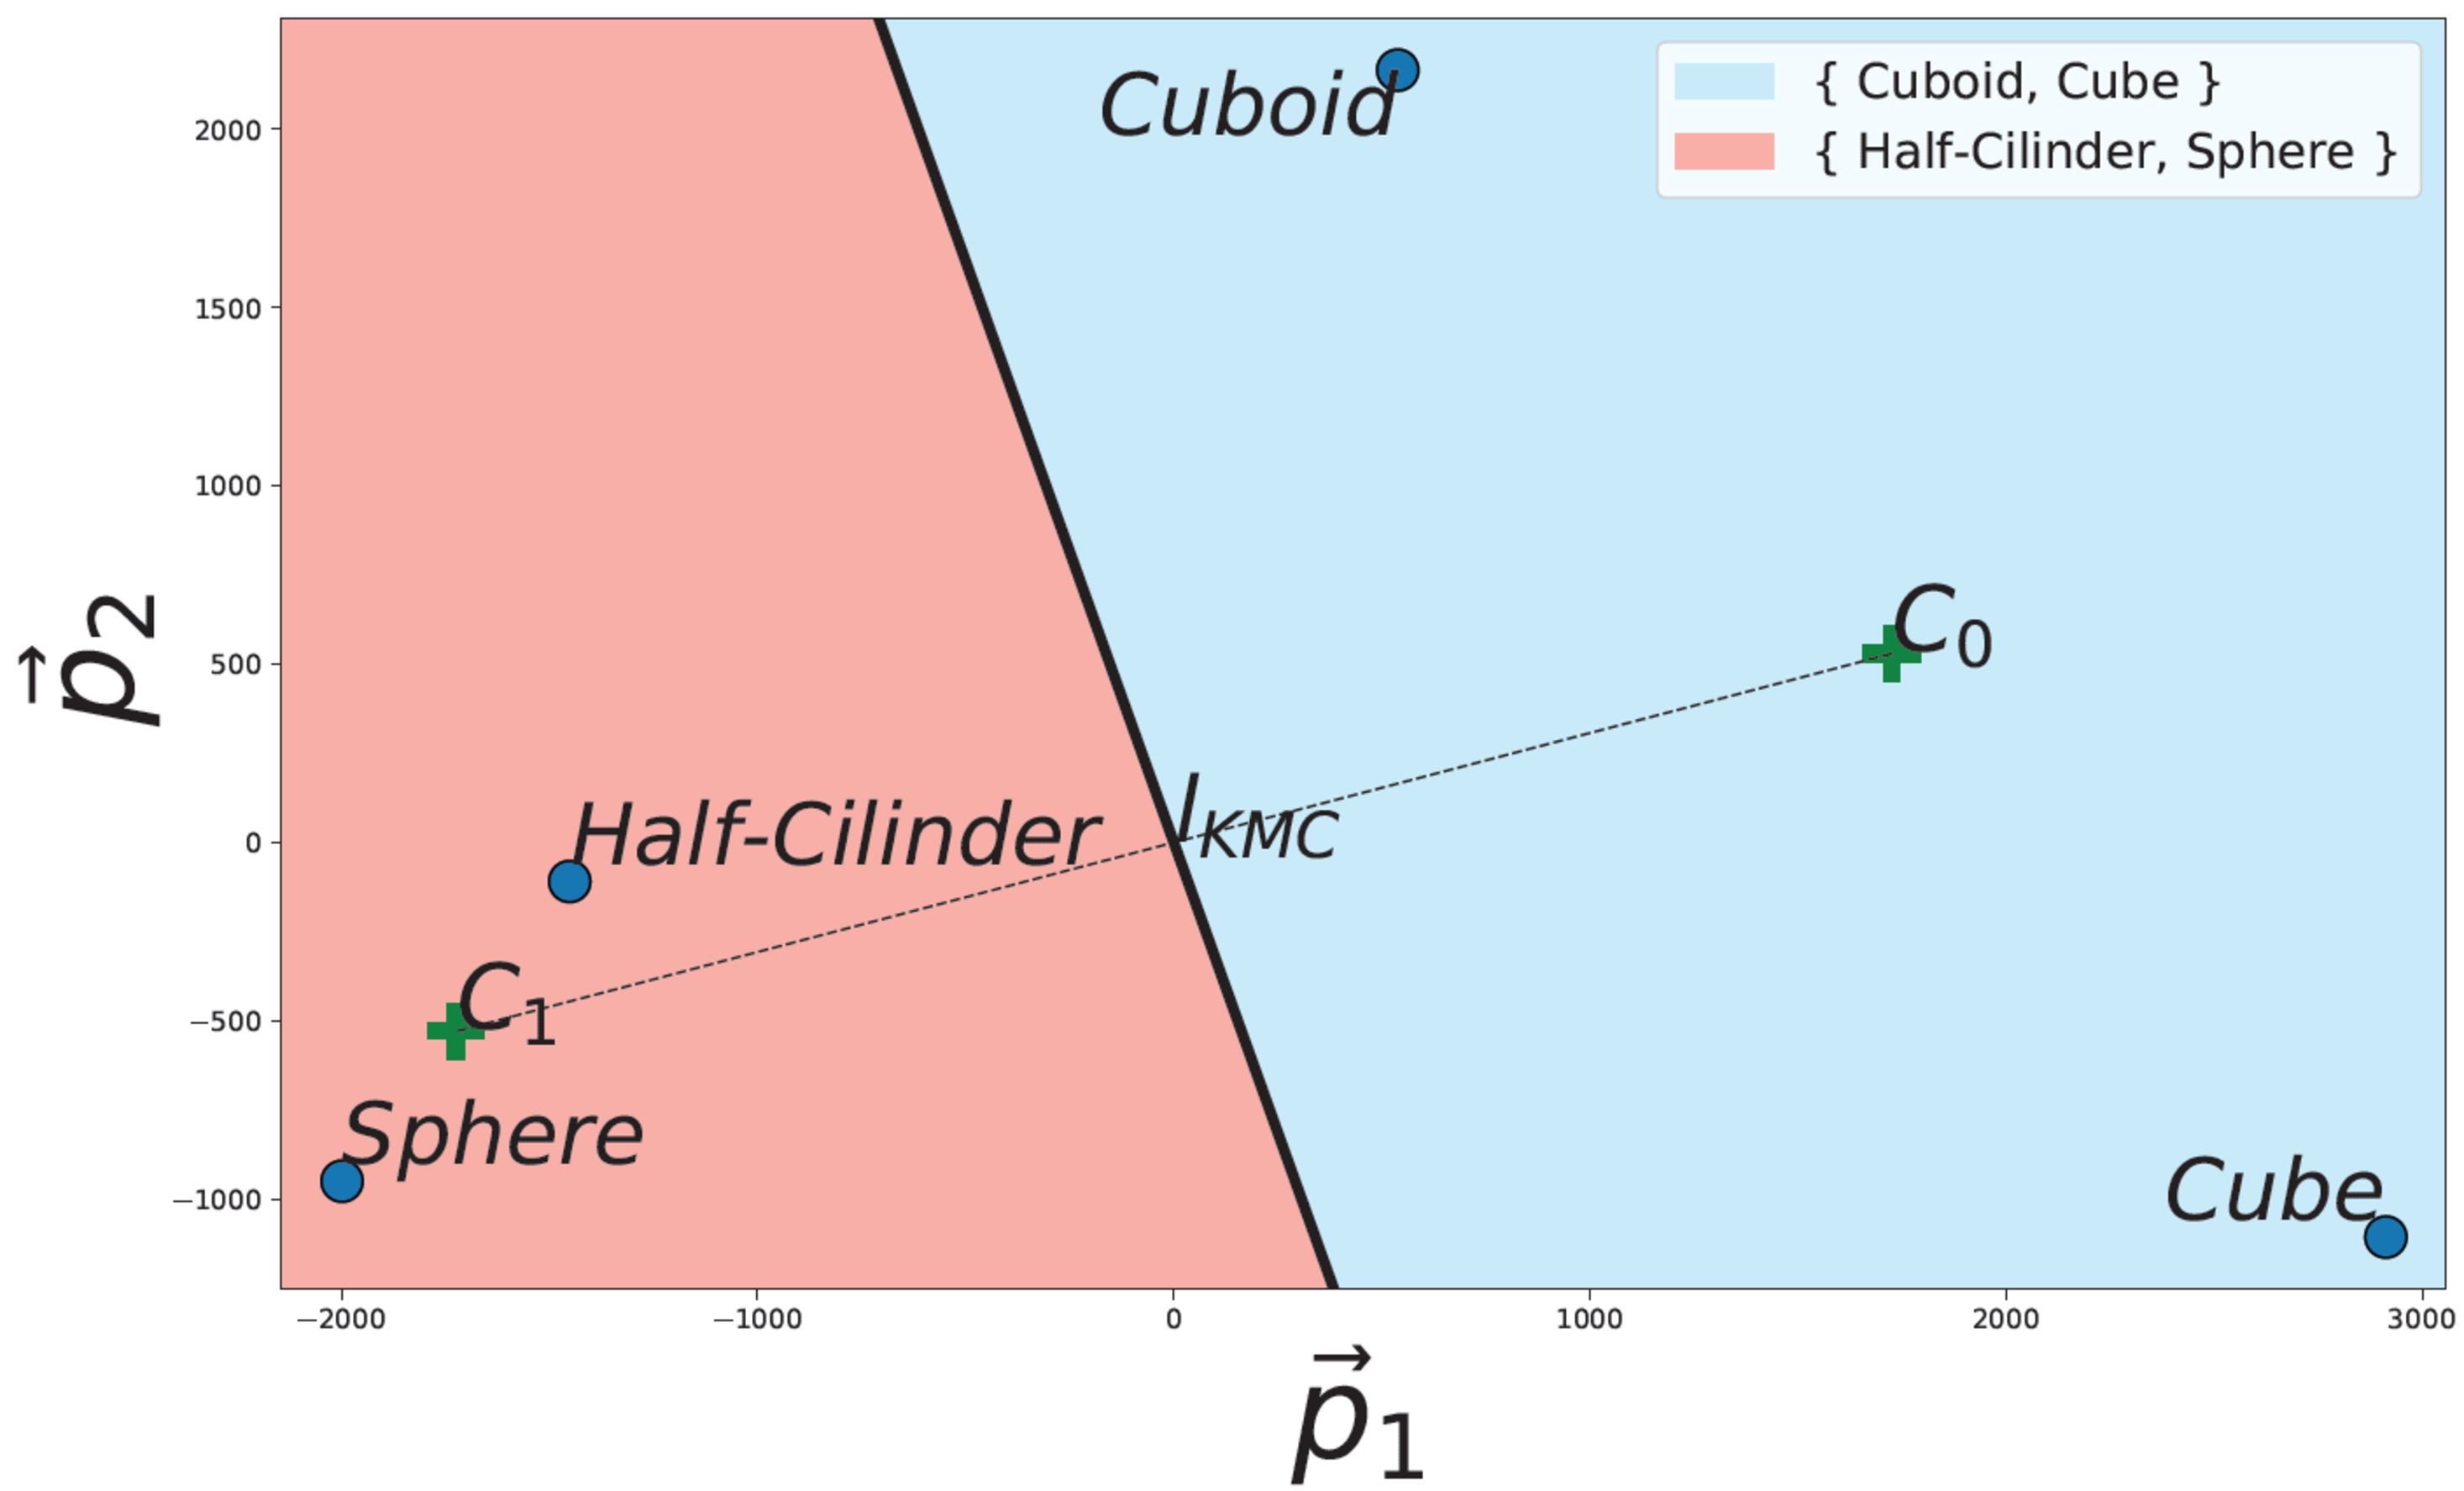
\includegraphics[width=\textwidth]{./figs/plt_3mm.pdf}
		\caption{}
		\label{plots:3mm}
	\end{subfigure}  
	\begin{subfigure}[b]{0.407\textwidth}
		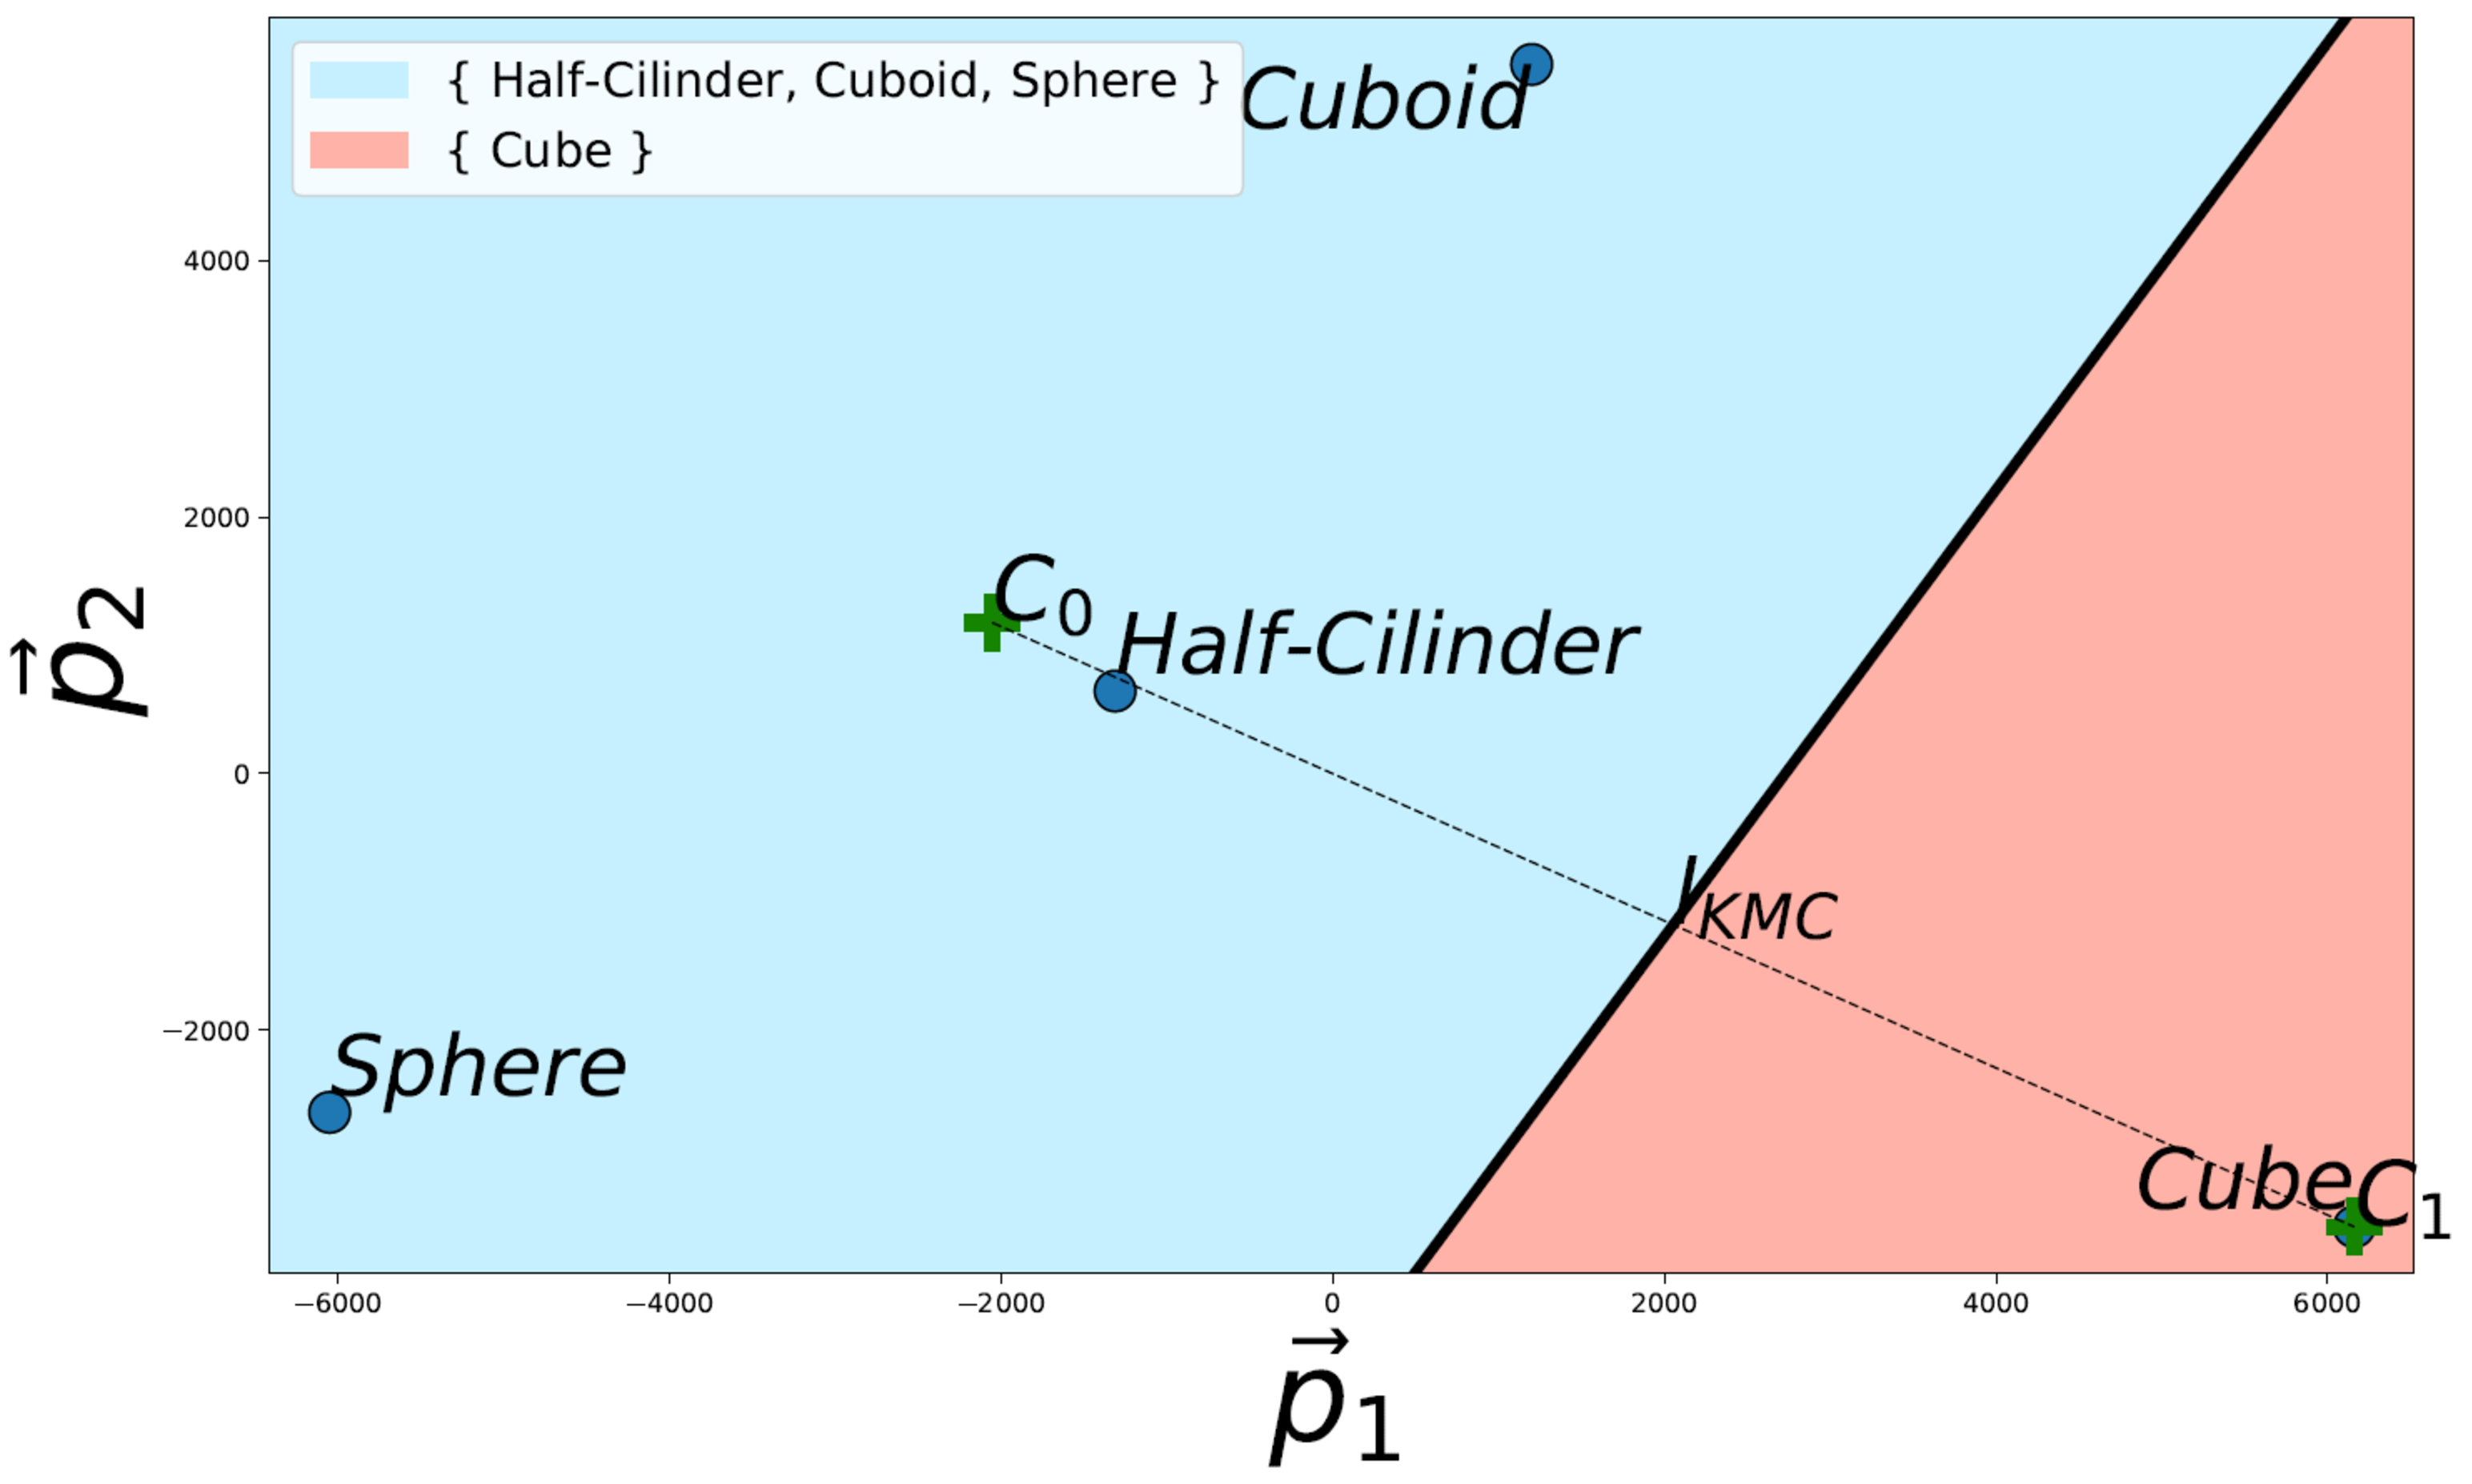
\includegraphics[width=\textwidth]{./figs/plt_6mm.pdf}
		\caption{}
		\label{plots:6mm}
	\end{subfigure}
	\begin{subfigure}[b]{0.4\textwidth}
		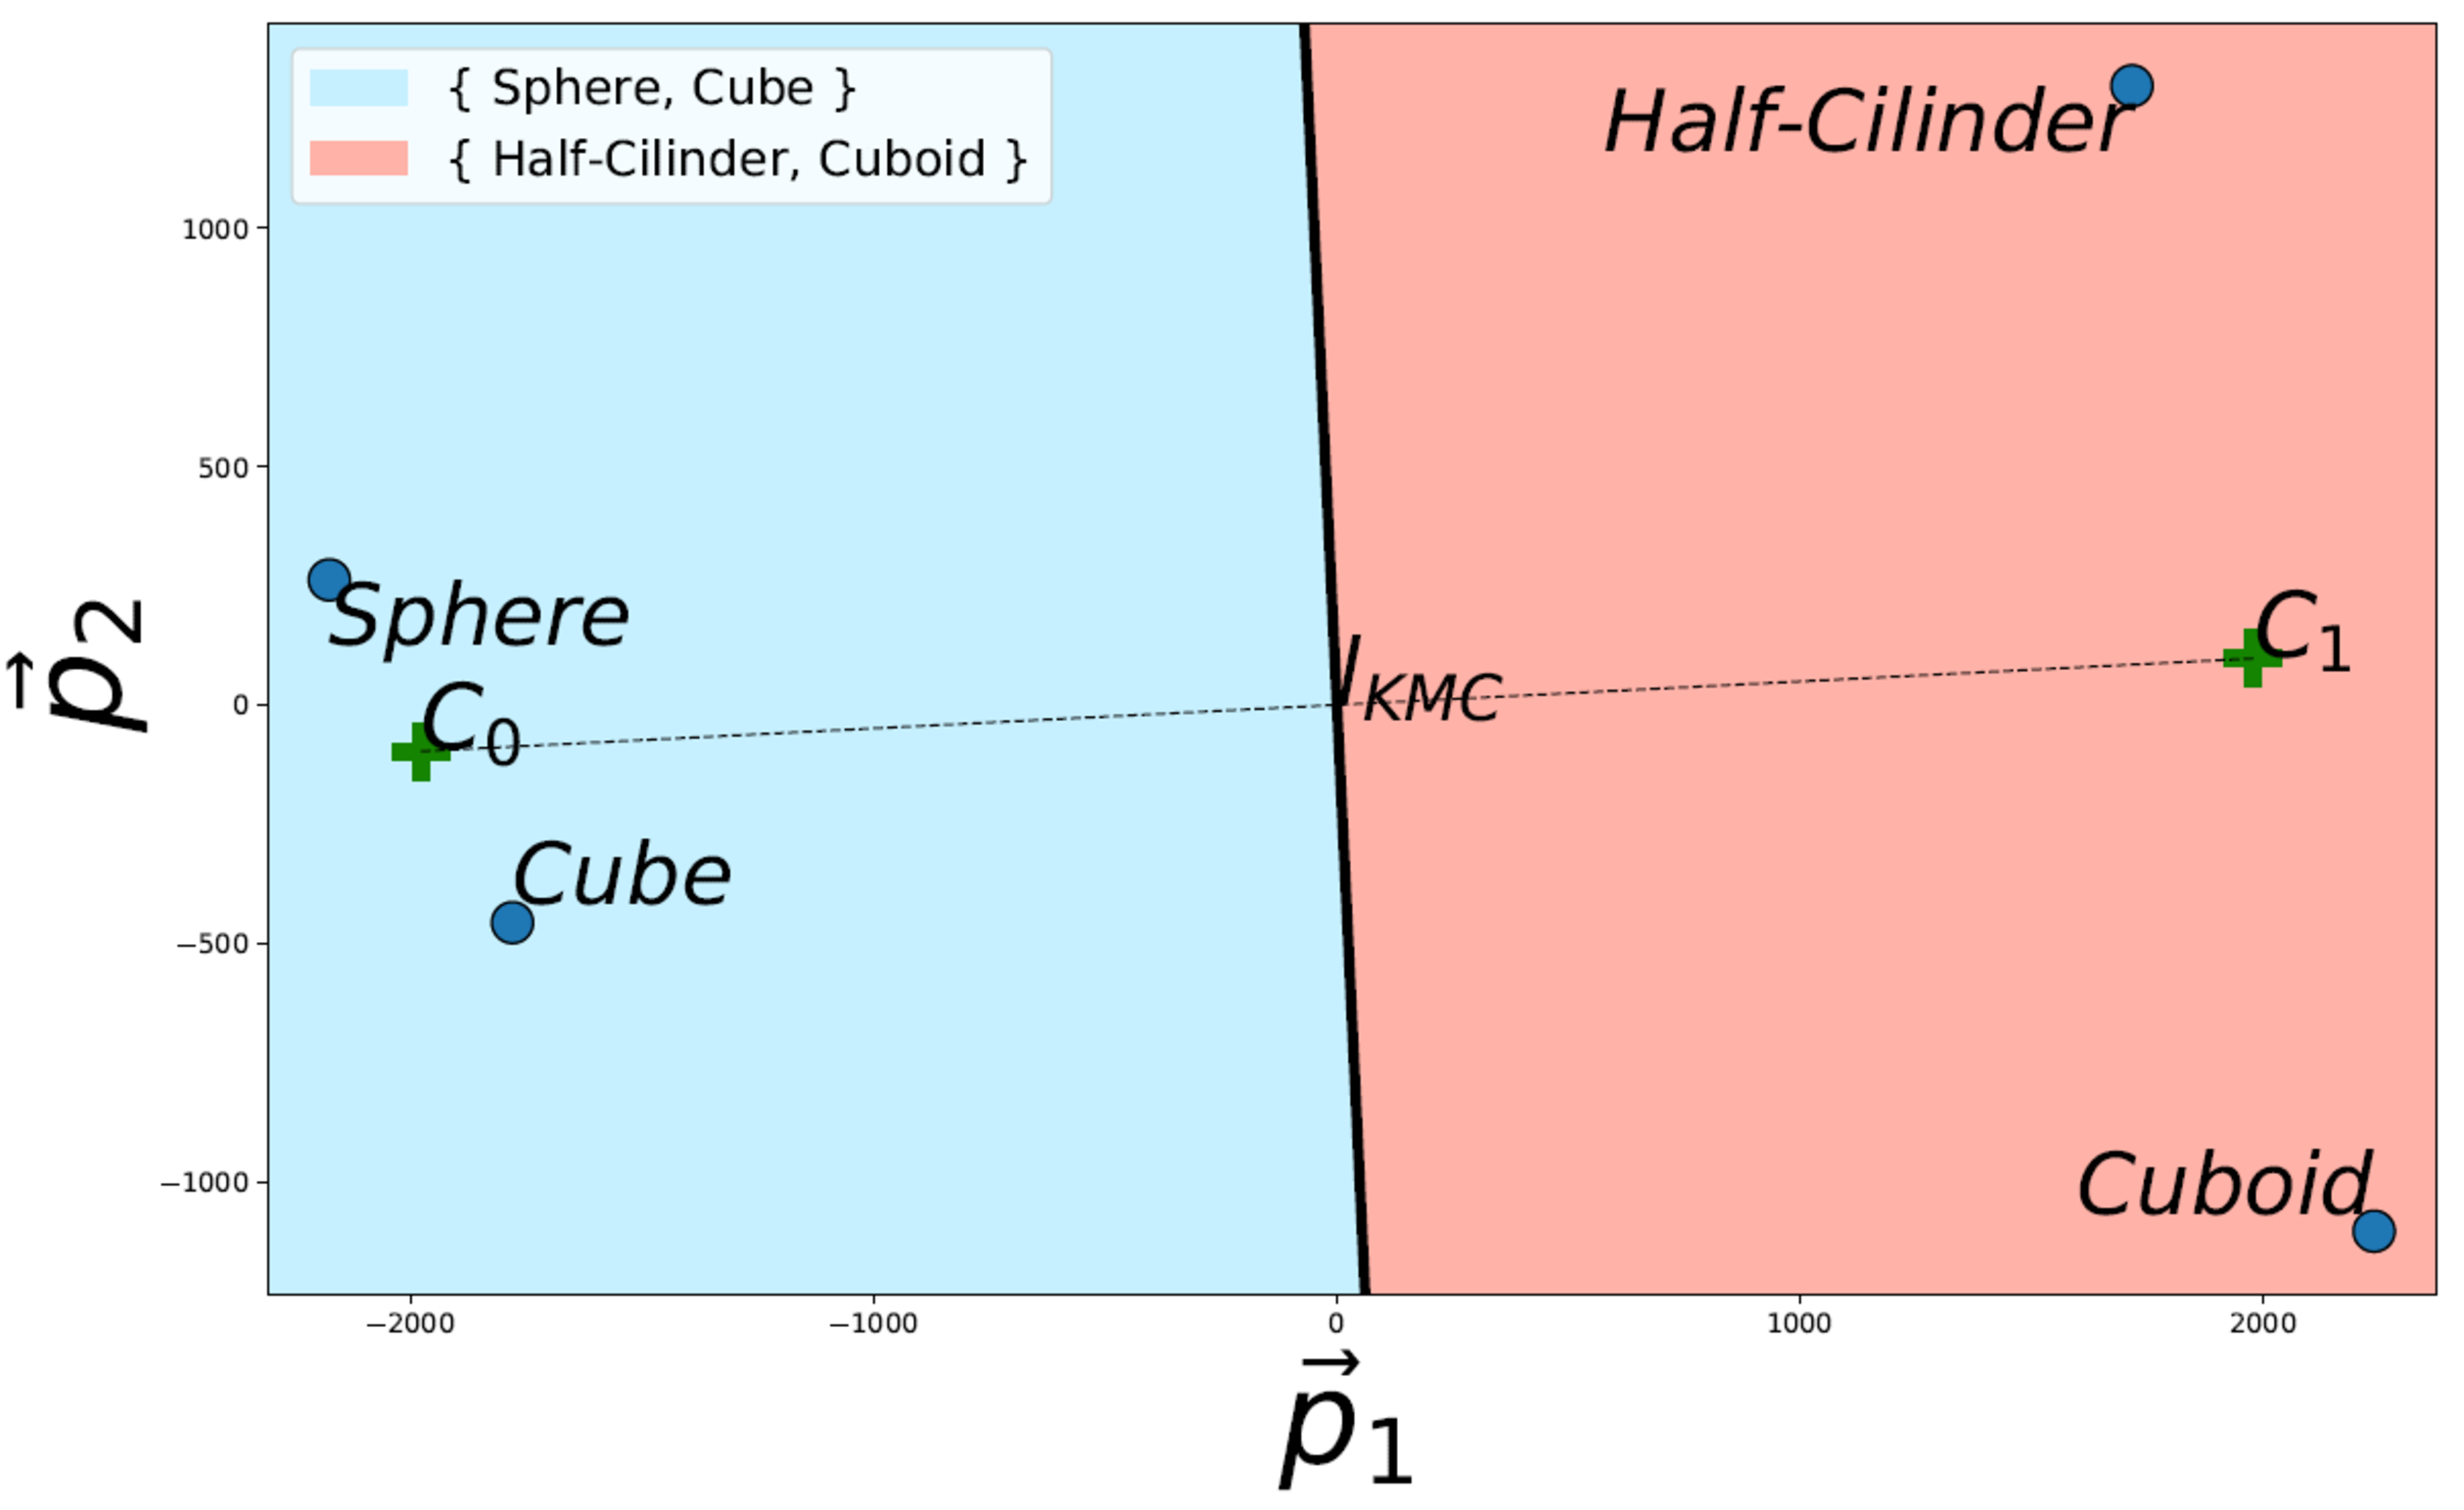
\includegraphics[width=\textwidth]{./figs/plt_1cm.pdf}
		\caption{}
		\label{plots:10mm}
	\end{subfigure}
	\caption{The figure shows the 2-dimensional projection of each object on the two axis of highest variance in the data for the $3mm$ soft filter (a), $6mm$ soft filter (b) and $10mm$ soft filter (c). The line $l_{kmc}$ corresponds to the decision boundary of the two clusters as found by the $KMC$ algorithm (see Section \ref{sec_unsup_clustering}, equation (\ref{kmc_eq})), while $C_0$ and $C_1$ represent the cluster centroids. From the figure is it clear how the relative distance between objects changes when changing the soft filter, and the corresponding cluster assignment through the $KMC$ algorithm. }
	\label{plots}
\end{figure}
\noindent the clustering process significantly. The tactile images taken through the $3mm$ soft filter optimize clustering for Task 5 ($accuracy=1$); The tactile images taken trough the $6mm$ soft filter optimize clustering for Task 2; and finally, sensing through the $10mm$ filter clusters optimally according to Task 6. 
\subsection{Autonomous Category Formation variations}
Fig. \ref{plots} illustrates the plots for each object in their optimal matched tasks. In the figure, the relative position of the objects to each other changes according to the soft filter used, drawing closer objects with respect to the morphologically processed features. The descriptions retrieved from the $3mm$ soft filter encode information relative to edges, and therefore draw together in space objects with or without edged surfaces (Cube \& Cuboid vs Sphere \& Half-Cilinder). As the thickness of the soft filter increases, the tactile sensor response becomes more blurred \cite{shimojo_mechanical_1997}. 
With thicker soft filters ($10mm$) the propagation of forces in the filter changes, and neighboring taxels to the ones directly under the object are also affected. As edges, in a tactile image, become less and less sharp, another parameter (i.e. length) comes to induce the highest change in sensor readings from object to object. As a direct consequence the dimensions of highest variance, appointed by PCA, change from encoding edge information to encoding length deviations of objects, and eventually draw close in space the representation of objects with similar lengths (Cube \& Sphere vs Cuboid \& Half-Cilinder). 

\begin{figure}[]
	\centering
	\begin{subfigure}[b]{0.45\textwidth}
		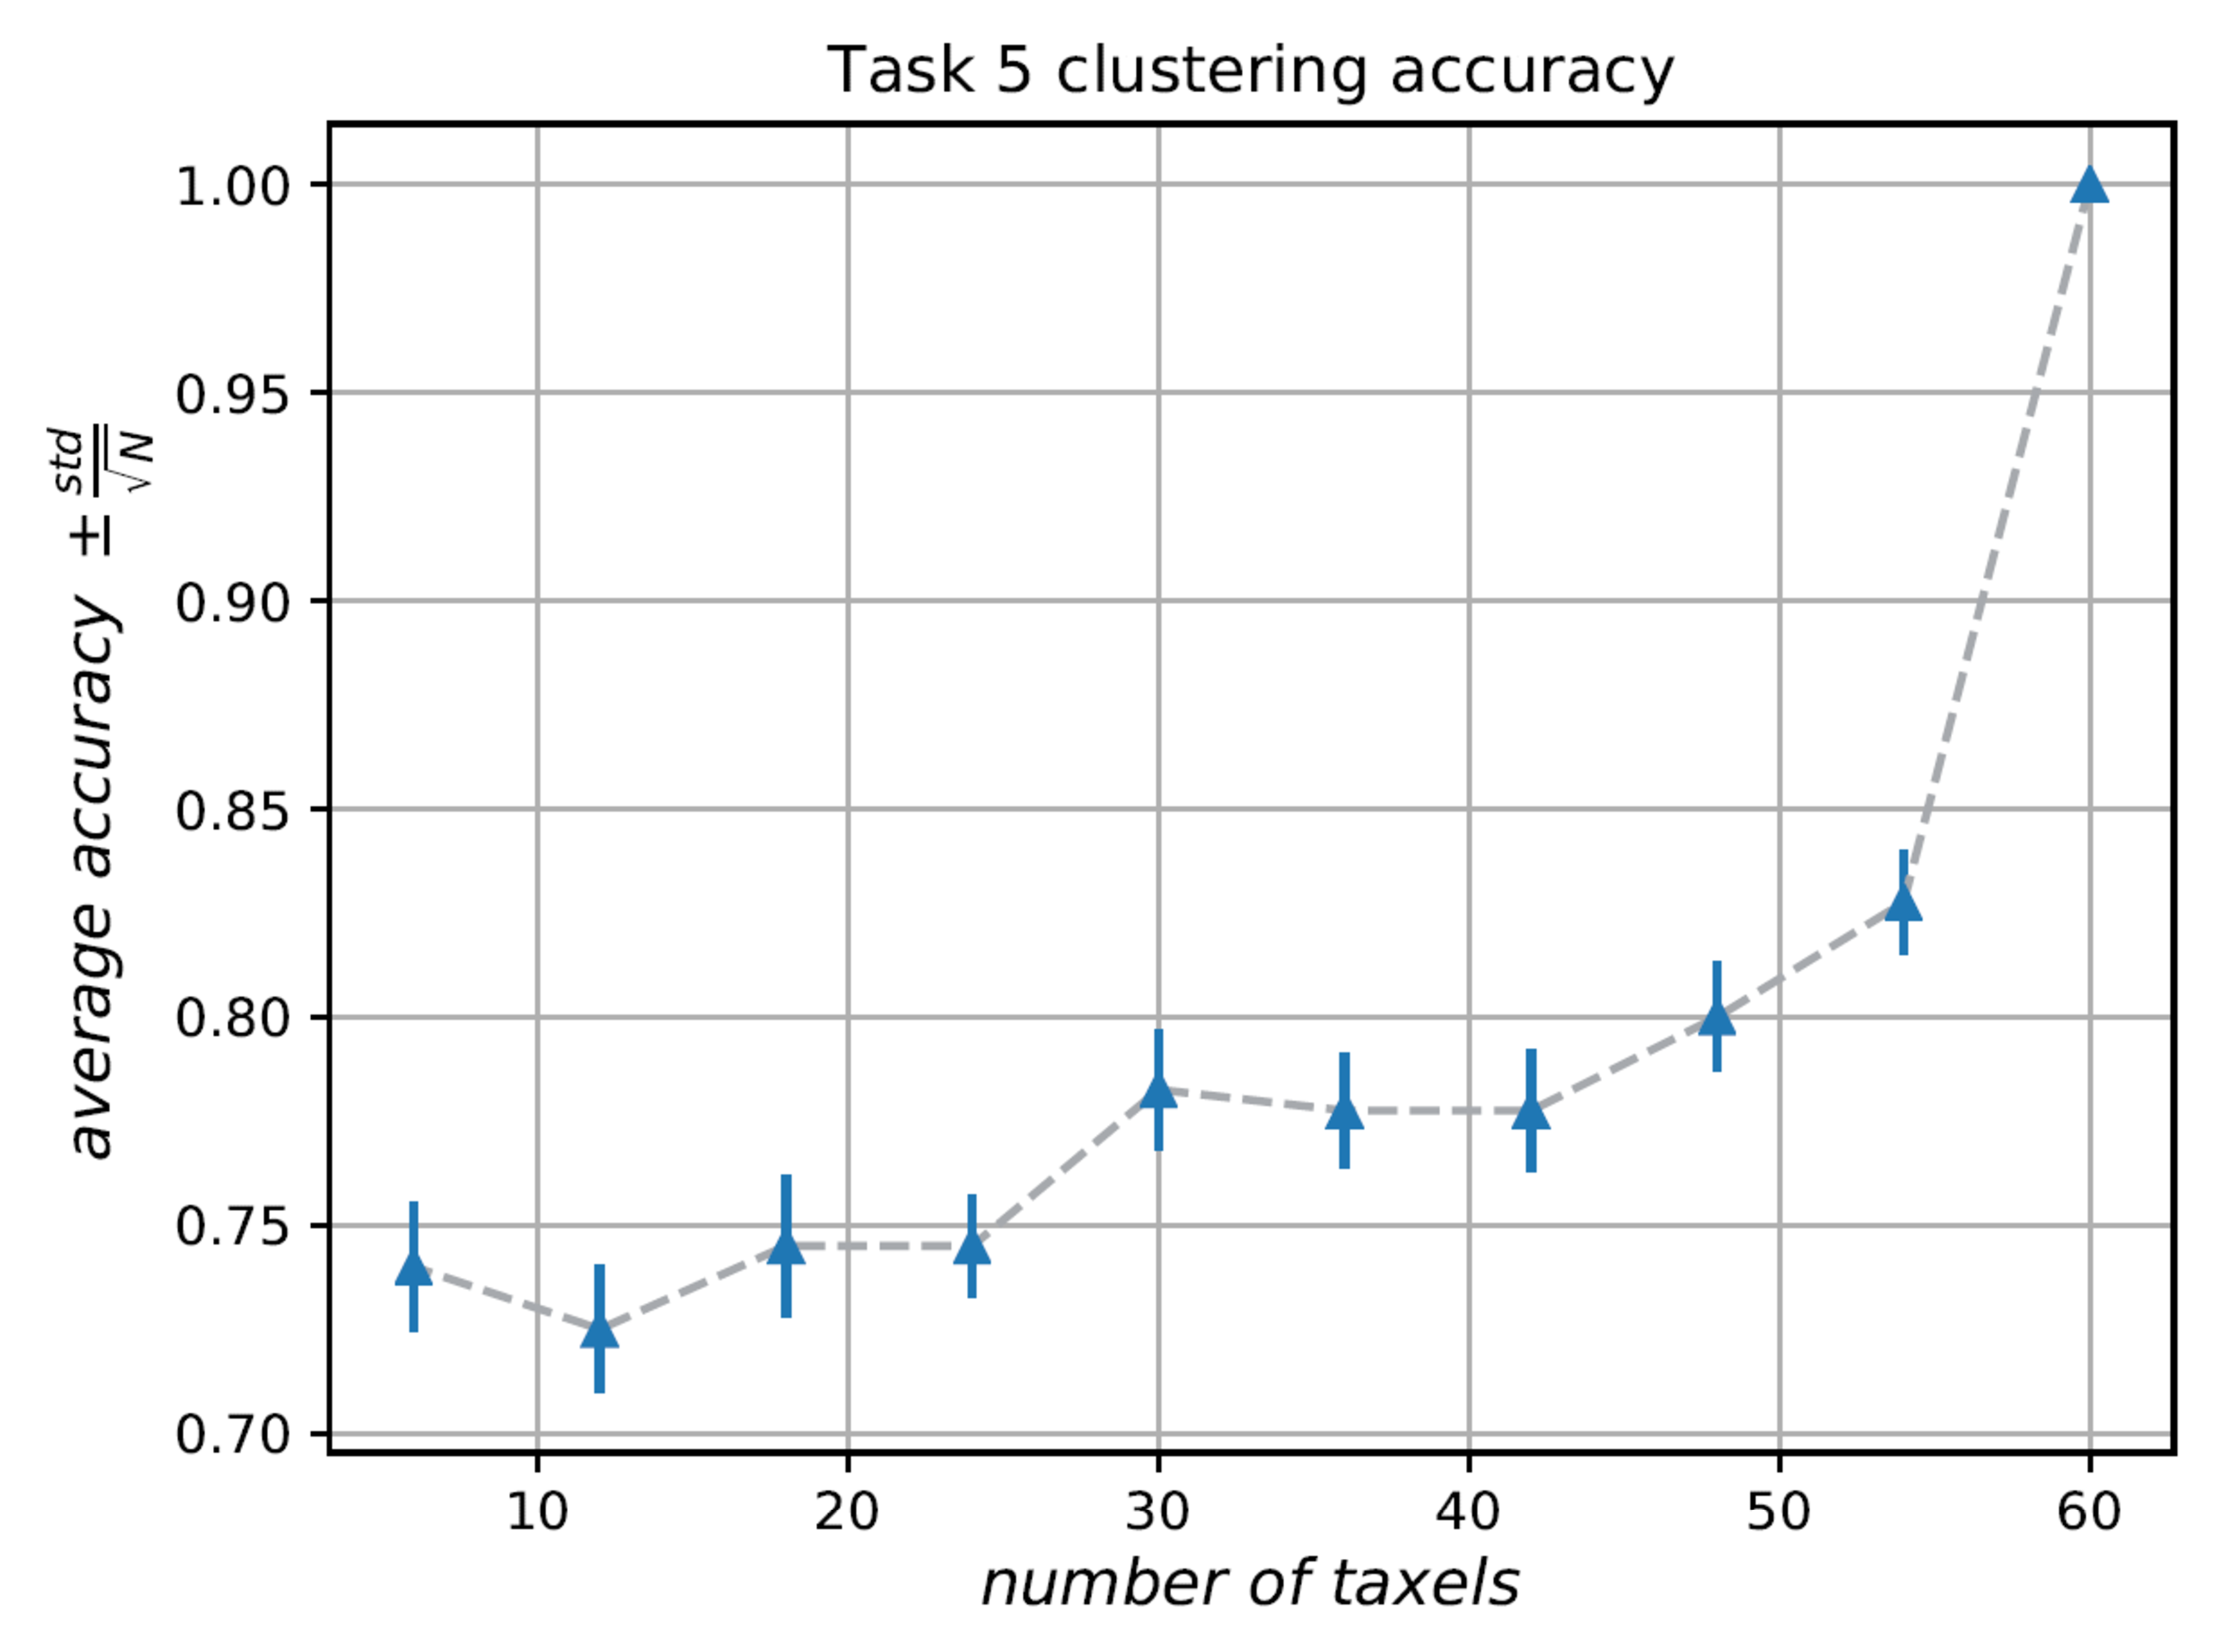
\includegraphics[width=\textwidth]{./figs/Task5_accuracy_map.pdf}
		\caption{}
		\label{accuracy:TAs}
	\end{subfigure}
	\begin{subfigure}[b]{0.45\textwidth}
		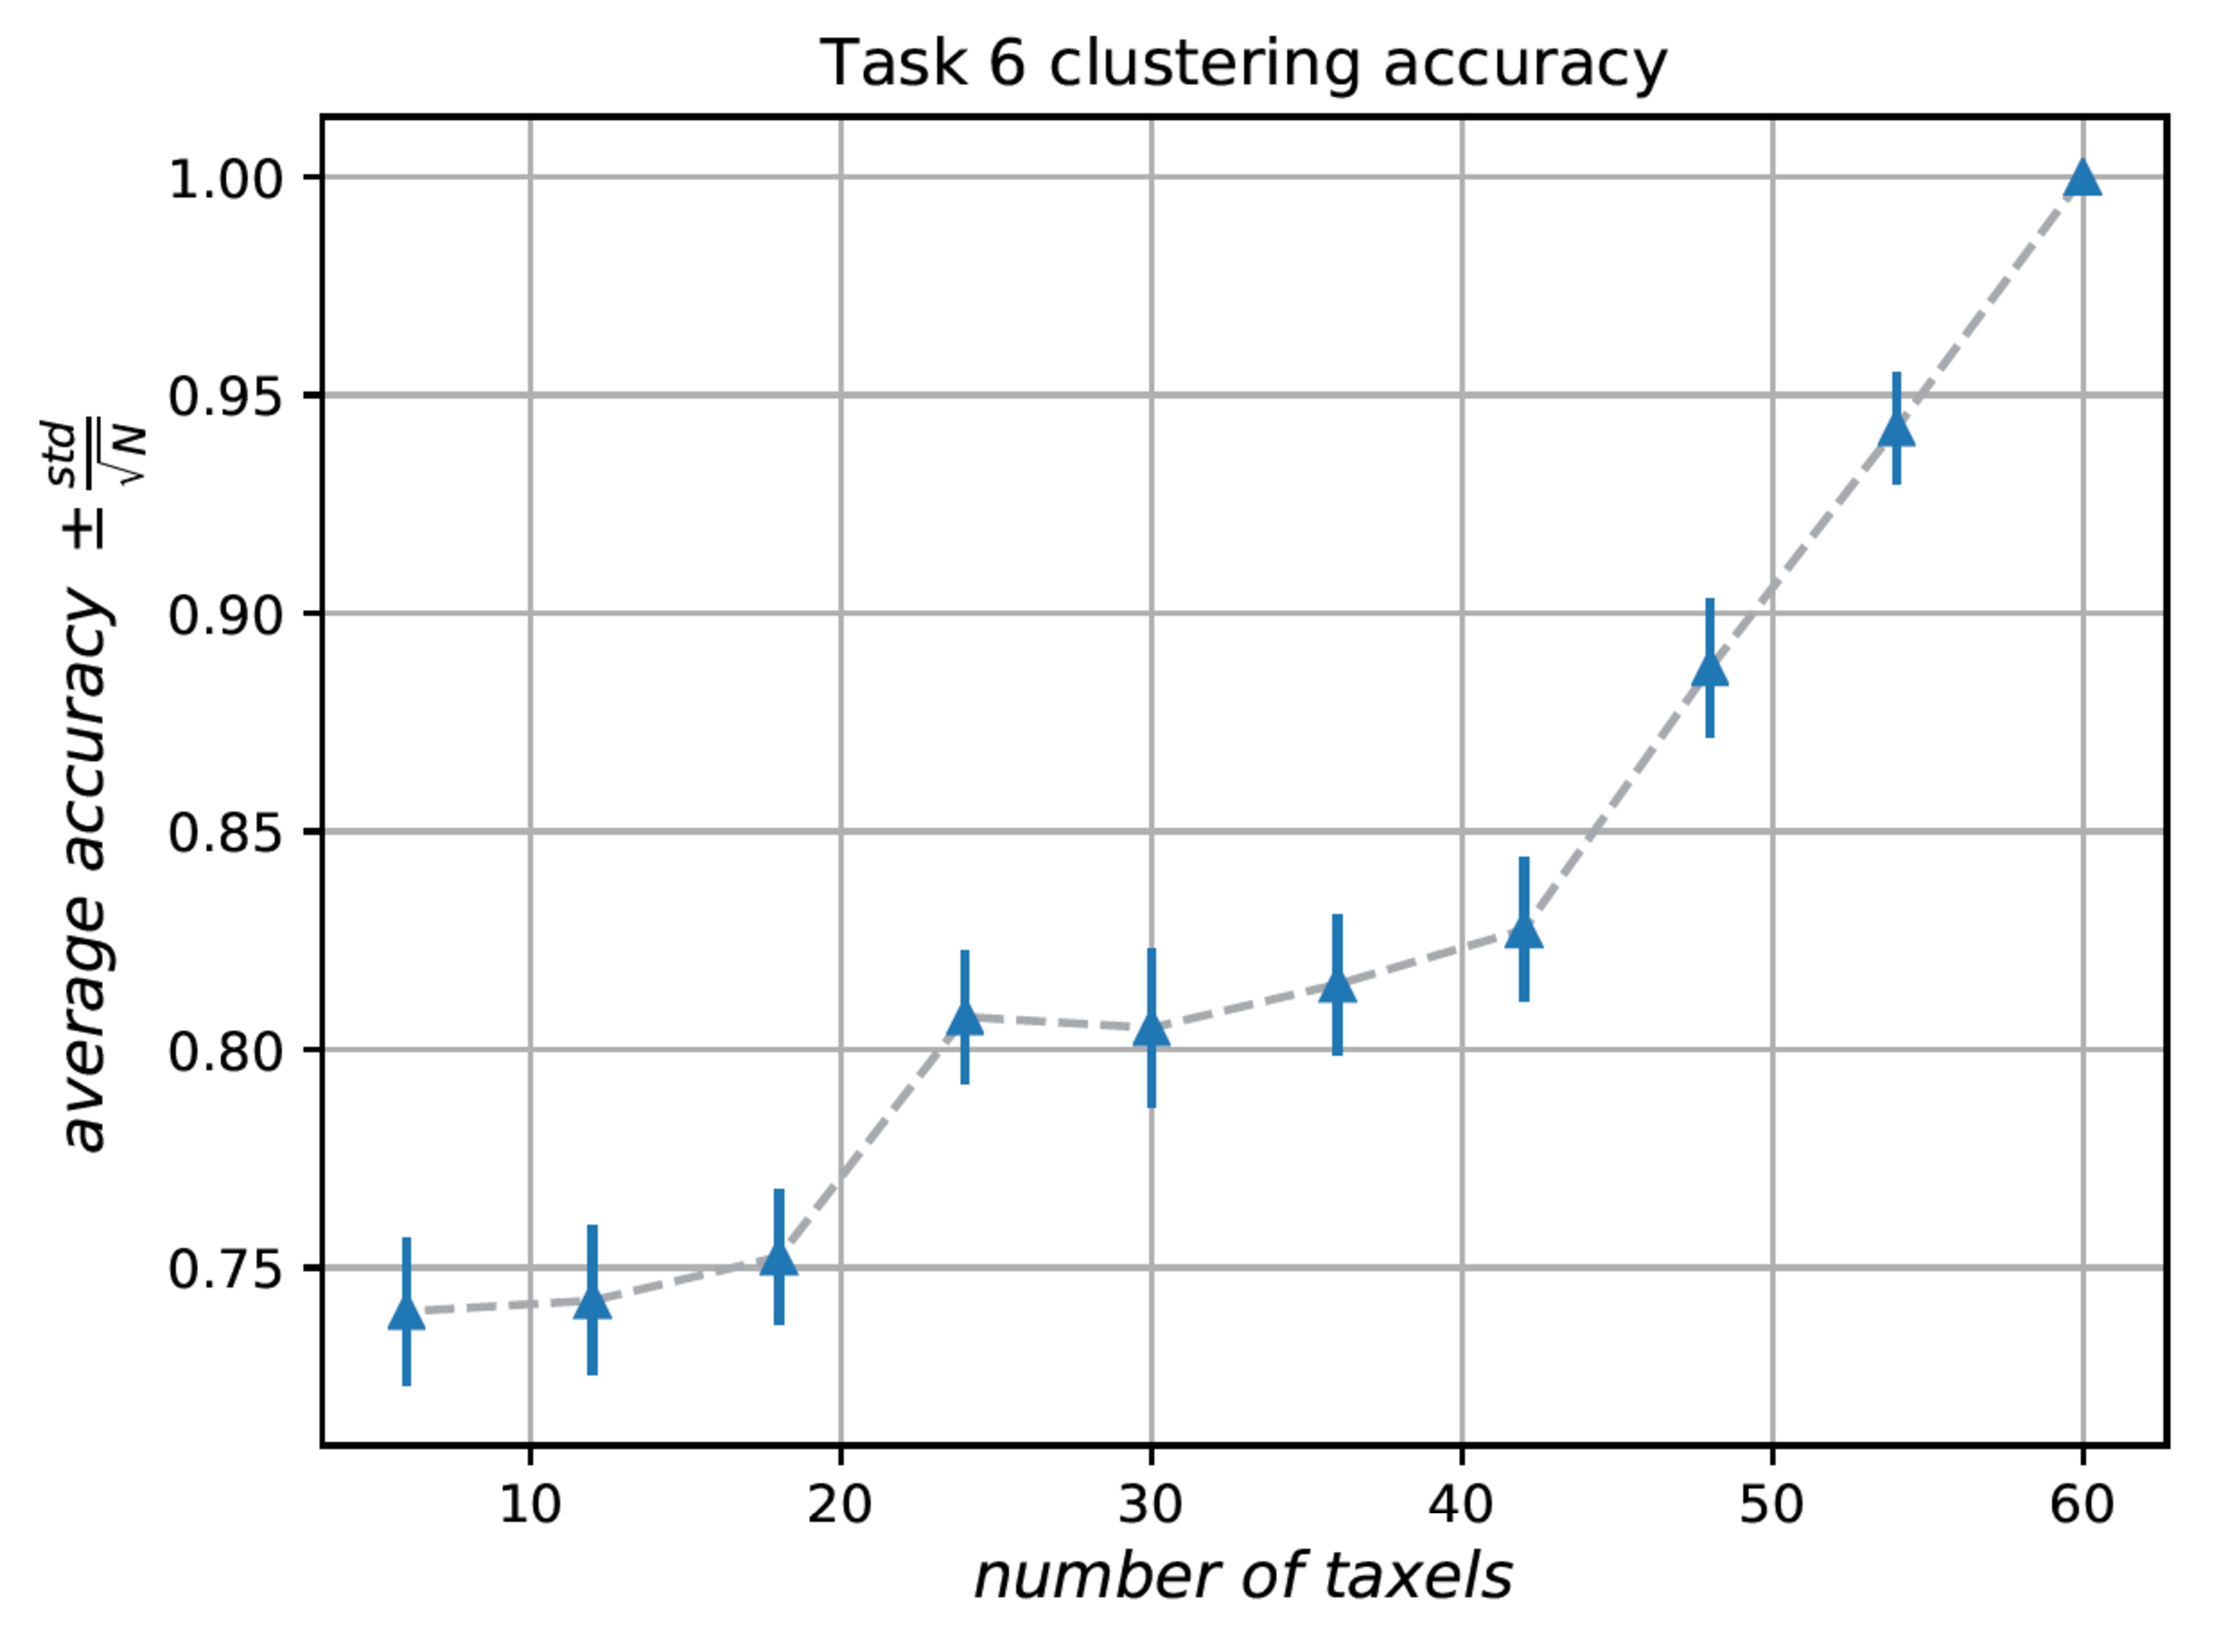
\includegraphics[width=\textwidth]{./figs/Task6_accuracy_map.pdf}
		\caption{}
		\label{accuracy:objects}
	\end{subfigure}
	\caption{The figure reports the average accuracy and error $e=\pm \frac{\sqrt{std}}{N}$) for the inference algorithm to cluster according to Task 4 (a) and Task 5 (b), when morphologically processing the data with their respective optimal filters ($3mm$ soft filter and $10mm$ soft-filter respectively).}
	\label{accuracy}
\end{figure}

\subsection{Spatial Resolution Influence}
We test the reliability of the findings over tactile spatial resolution by running the Autonomous Category Formation procedure over subsets of $s$ selected taxels. For each subset, we randomly select within the sensor an increasing number of taxels, where $s \in \{6i|\ i\in{1, ... , 6}\}$, and run the procedure 100 times. In Fig. \ref{accuracy}, we report the average accuracy levels and errors over the performed runs for the optimal soft filter in Task 5 ($3mm$ filter) and Task 6 ($10mm$ filter). 
We find that the ability to morphologically process the data is highly dependent on the spatial resolution of the tactile sensor and that results are best when using $\approx 50$ or more taxels. The findings highlight the need of a high spatial resolution tactile sensor for the analysis described in this paper.


\section{DISCUSSION}
\label{sec_discussion}
After morphologically processing the tactile stimuli, we observe inherently different cluster guesses. Each soft filter alters the sensor response significantly, and induces the object descriptions (based on the two dimensions of highest variance in the data) to be qualitatively largely different.
The experiments provide direct evidence of how changing a single parameter of a soft filter can drastically change the way we perceive objects in the world. In the context of understanding relations amongst objects (for example clustering objects based on different features), the standard approach in the field is to change the inference mechanism to implicitly discern among features. Many of the used algorithms, in fact, need a large amount of data (usually labeled) which allows them to build an internal model of the objects and later do inference on the same. Understanding object properties in an unsupervised manner can be appealing, as there is no need of labeling or explicit modeling throughout the process. The experiments suggest we can drive the unsupervised findings by a careful design of the soft filters for a tactile sensor. As an indirect consequence, we show it is possible to optimize the tactile sensor's soft filter to drive the unsupervised inference algorithm into creating a useful world representation. In the context of manipulation or gripping mechanisms, for example, we may wish to grip an object based on a set of two or more properties. A soft filter can then be carefully designed to be optimal in extracting only the most relevant information for a task while filtering the others. The resulting clusters, then, would be retaining the feature information in terms of object similarities. By simple reinforcement learning, or other more involved strategies, a robot could then learn to grip an object in a cluster, and possibly generalize the gripping mechanism easily on other members of the cluster. In this scenario, no other information, besides cluster membership, would need to be known, and the human input in the process would be minimal.

\section{CONCLUSION}\label{sec_conclusion}
We propose a concept to examine the way morphology affects the encoding of tactile sensor stimuli and analyze its effects on category formation. We actualize the concept by developing an unsupervised method for clustering  a set of objects into two clusters. After integrating a capacitive tactile sensor onto a custom 3D-printed end-effector, we change the properties of a soft filter to alter the tactile stimuli and observe the change in cluster formation derived from the alteration. Results show that changing one parameter of the soft filter is enough to provide three qualitatively different representations of the objects. When clustering, we find the inference procedure relies on different object properties depending on the morphological processing applied. In this context, the $3mm$ soft filter optimizes the inference procedure for edge detection while the thicker $10mm$ object results optimal for elongation detection. A test on the reliability of the findings over various randomly selected set of taxels shows the results are highly dependent on the tactile spatial resolution of the sensor.



\addtolength{\textheight}{-12cm}   % This command serves to balance the column lengths
%                                  % on the last page of the document manually. It shortens
%                                  % the textheight of the last page by a suitable amount.
%                                  % This command does not take effect until the next page
%                                  % so it should come on the pagse before the last. Make
%                                  % sure that you do not shorten the textheight too much.

%%%%%%%%%%%%%%%%%%%%%%%%%%%%%%%%%%%%%%%%%%%%%%%%%%%%%%%%%%%%%%%%%%%%%%%%%%%%%%%%


\bibliographystyle{IEEEtran} % use IEEEtran.bst style
\bibliography{IEEEabrv,IEEEexample}

%%%%%%%%%%%%%%%%%%%%%%%%%%%%%%%%%%%%%%%%%%%%%%%%%%%%%%%%%%%%%%%%%%%%%%%%%%%%%%%%


%%%%%%%%%%%%%%%%%%%%%%%%%%%%%%%%%%%%%%%%%%%%%%%%%%%%%%%%%%%%%%%%%%%%%%%%%%%%%%%%
\end{document}
